%% Main Master Thesis Document
%% Progress draft: complete through Evaluation Method (EDA + dual-system pipeline + protocol).
%% Results/Discussion/Conclusion pending full-scale verification of all three generators.
%% Rebuild EDA figures: python code/scripts/generate_thesis_figures.py
%% Writing notes: THESIS_WRITING_NOTES.md

\documentclass{srhthesis}

% Packages you intend to use
% ..

% For example, if you want to render 
% the document in a different font you can
% use something like: 

% \usepackage{gentium}

\usepackage{url}
\usepackage{xurl}
\usepackage{booktabs}
\usepackage{tikz}
\usetikzlibrary{arrows.meta,positioning,fit,shapes.geometric}

\usepackage{listings}
\usepackage{xcolor}
\lstdefinestyle{thesispy}{
  language=Python,
  basicstyle=\ttfamily\footnotesize,
  keywordstyle=\bfseries\color{blue!50!black},
  commentstyle=\itshape\color{black!50},
  stringstyle=\color{green!40!black},
  numbers=left,
  numberstyle=\tiny\color{black!40},
  numbersep=8pt,
  frame=single,
  rulecolor=\color{black!20},
  breaklines=true,
  breakatwhitespace=false,
  showstringspaces=false,
  tabsize=4,
  columns=flexible,
  xleftmargin=1em,
}
\lstset{style=thesispy}
% Main thesis metadata (distinct from the proposal document)
\author{Raja Karthik Chirumamilla}
\thesisDegree{Masters in Computer Science (Big Data and Artificial Intelligence)}
\thesisSubmissionDate{April, 2026}

\title{\bfseries
Dual-System Hallucination-Free Legal Document Summarization:
A Neuro-Symbolic Framework for Legal Summarization with Verifiable Case Citations}

\thesisSupervisor{Prof. Dr. Fakhteh Ghanbarnejad}
\thesisSecondSupervisor{Prof. Mohandoss Smitha}

\thesisProgramme{Computer Science (Big Data and Artificial Intelligence)}
\thesisSchool{School of Technology Leipzig}
\thesisUniversity{SRH University of Applied Sciences}

% Add in the .bib files you wish to add 
% into your document here. If you want to
% include others, just copy this line and
% change the path!

\addbibresource{bib/references.bib}


% This thesis template also supports rendering
% a ludography. To cite games, make sure your reference
% in your bib file has keywords={game} in the bibtex item.
%
% See the bib file below for an example.

\addbibresource{bib/ludography.bib}

\graphicspath{{figures/eda/}{figures/results/}{figures/methodology/}}

\begin{document}

\maketitle

\begin{abstract}
Legal AI systems summarize long case records, and fabricated or incorrect case citations in those summaries cause serious professional harm. Prior work documents high hallucination rates in public large language models and in commercial retrieval-augmented legal research tools \cite{dahl2024largelegalfictions,magesh2025hallucinationfree}. Multi-LexSum shows the same problem from another angle: strong ROUGE scores on legal multi-document summarization coexist with very low human faithfulness ratings \cite{shen2022multilexsum,maynez2020faithfulness}. This thesis builds a dual-system, neuro-symbolic pipeline that generates long legal case summaries with PRIMERA, extracts case citations with eyecite, verifies them against CourtListener, and applies a bounded symbolic correction policy (redaction, safe repair, same-case re-anchoring) before release.\footnote{Code, aggregate results, and a live demo: \href{\repourl}{\repourl}.}

Exploratory data analysis on the full Multi-LexSum corpus (4{,}539 cases) sets the empirical terms for the design. Source documents run extremely long and truncation is unavoidable; short and tiny expert labels are incomplete; long summaries carry substantially higher citation density than the other two granularities. These three findings justify the document-to-long ($D\rightarrow L$) task and the decision to treat the neural summarizer as an \emph{untrusted} draft generator. The methodology chapter specifies Modules~A--C, the Verified/Mismatch/Ambiguous/NotFound/Malformed taxonomy, paired draft-citation hallucination rate as the primary faithfulness metric, and correction rules that never substitute a contradicting CourtListener case name.

Full-scale evaluation covers three Module~A generators (PRIMERA, an LLM zero-shot variant, and an LLM+retrieval variant) on the same 100 citation-dense Multi-LexSum test-split cases, testing whether citation-hallucination behaviour belongs to one checkpoint or generalizes across generator architecture. Baseline paired hallucination rate is substantial in every generator, 57.5 to 82.8\%. Symbolic verification and bounded correction reduce it by 56.1 to 71.8\% relative to baseline ($p<10^{-4}$, McNemar, all generators). Across 1{,}083 paired citations evaluated, correction makes \emph{zero} citations worse. Summarization quality survives with wide margin: ROUGE-L\textsubscript{sum} moves by at most 0.07 percentage points against a $\pm2$pp tolerance, and BERTScore~F1 by at most 0.0003. The correction policy was built and tuned against PRIMERA's low-volume citation profile, yet it holds final hallucination rate to a narrow 22.2--27.6\% band across all three generators despite a 24$\times$ range in citation volume between them. The approach generalizes; it was not overfit to one generator. A qualitative analysis also finds a degenerate citation-fabrication failure mode that citation-density retrieval substantially suppresses, from 13.7\% to 0.7\% of citations affected. Human-in-the-loop validation of the automated taxonomy and of corrected-summary readability remains immediate future work.

\end{abstract}

\thesisTables

\cleardoublepage
\addcontentsline{toc}{chapter}{List of Abbreviations}
\chapter*{List of Abbreviations}
\begin{longtable}{@{}p{3.2cm}p{10cm}@{}}
\toprule
\textbf{Abbreviation} & \textbf{Meaning} \\
\midrule
\endhead
AI & Artificial Intelligence \\
API & Application Programming Interface \\
AUC & Area Under the (ROC) Curve \\
BART & Bidirectional and Auto-Regressive Transformer \\
BERT & Bidirectional Encoder Representations from Transformers \\
BLEU & Bilingual Evaluation Understudy \\
CC BY-NC & Creative Commons Attribution-NonCommercial (licence) \\
CI & Confidence Interval \\
CL & CourtListener \\
CRLC & Civil Rights Litigation Clearinghouse \\
$D \rightarrow L$ & Document-to-Long (summarization task) \\
$D \rightarrow S$ & Document-to-Short (summarization task) \\
$D \rightarrow T$ & Document-to-Tiny (summarization task) \\
DUC & Document Understanding Conference \\
EDA & Exploratory Data Analysis \\
EM & Exact Match \\
GPT & Generative Pre-trained Transformer \\
GPU & Graphics Processing Unit \\
HR & Hallucination Rate \\
HTML & HyperText Markup Language \\
LCS & Longest Common Subsequence \\
LLM & Large Language Model \\
MDS & Multi-Document Summarization \\
NLG & Natural Language Generation \\
NLI & Natural Language Inference \\
NLP & Natural Language Processing \\
NQ & Natural Questions (dataset) \\
OCR & Optical Character Recognition \\
PRIMERA & Pyramid-based Masked Sentence Pre-training for Multi-document Summarization \cite{xiao2022primera} \\
QA & Question Answering \\
QG & Question Generation \\
RAG & Retrieval-Augmented Generation \\
ROC & Receiver Operating Characteristic \\
ROUGE & Recall-Oriented Understudy for Gisting Evaluation \\
RQ & Research Question \\
SOTA & State of the Art \\
YAML & YAML Ain't Markup Language (configuration file format) \\
\bottomrule
\end{longtable}


\thesisBodyStart

\chapter{Introduction}
\section{Background}
\label{sec:intro-background}

Legal research is moving toward large language models, and that move carries a contradiction common to other high-stakes domains. These systems generate fluent text at unprecedented scale, and fluency is a poor proxy for reliability. Ankur Mali's dual-system thesis on industrial predictive maintenance argued that neural pattern recognition needs deliberative, domain-constrained reasoning to check it before any action follows. Legal summarization faces the same accountability gap. Behind every docket sits a physical litigation history. Behind every citation string sits a claim that a specific authority exists and says what the summary claims it says.

Legal practitioners, researchers, and non-specialist users increasingly rely on AI systems to search, summarize, and synthesize case records that routinely run hundreds of pages \cite{shen2022multilexsum}. Legal AI carries a professional constraint most consumer NLP applications do not: a fabricated or incorrect case citation can mislead courts, contaminate memoranda, and erode trust in automated tools \cite{dahl2024largelegalfictions,magesh2025hallucinationfree,lai2023llmslegal}.

This is a difference in kind, not degree, from other high-stakes NLP applications. A hallucinated statistic in a business report is wrong in isolation. A hallucinated case citation carries the rhetorical form of an authority: a specific court, at a specific time, deciding a specific question the way the summary claims. Legal reasoning runs on precedent, so a citation serves as the claim's evidentiary support, not decoration. A summarization system that gets the prose right but invents the authority produces a document that argues from evidence that does not exist. That distinction carries professional consequences, and disciplinary ones for a filed document.

\section{Problem Statement}
\label{sec:intro-problem}

Empirical work documents hallucination as a routine failure mode. When asked verifiable questions about federal court cases, public LLMs hallucinate at reported rates between 58\% and 88\% depending on the model \cite{dahl2024largelegalfictions}. Commercial retrieval-augmented legal research tools still hallucinate between 17\% and 33\% of the time in a preregistered evaluation \cite{magesh2025hallucinationfree}. Summarization raises the stakes further. Users often treat a summary as a substitute for reading the record, so a single invented authority can propagate into downstream reasoning.

Retrieval alone does not close this gap, and closing it is the central problem this thesis addresses. Grounding a model in retrieved passages constrains what it can draw from, but says nothing about what it asserts: a model can still misattribute a real holding to the wrong case, invent a plausible-sounding reporter string, or carry over a citation's party names while getting its year wrong. Magesh et al.'s 17--33\% figure for commercial RAG-based legal tools is itself evidence that retrieval reduces the problem without eliminating it \cite{magesh2025hallucinationfree}. Those systems need a check performed \emph{after} generation, against an authoritative source that can answer yes or no to a specific citation claim. That check is the gap this thesis's generate--verify--correct design targets.

Automatic summarization metrics systematically overestimate usefulness. Multi-LexSum reports competitive ROUGE for PRIMERA on document-to-long summarization while human faithfulness ratings for generations remain low, 0.43 on a 0--3 scale \cite{shen2022multilexsum}. Faithfulness studies in general-domain summarization show the same decoupling between overlap metrics and factuality \cite{maynez2020faithfulness,pagnoni2021factuality,kryscinski2020evaluating,honovich2022true}. The practical problem is how to make citation-bearing legal summaries \emph{auditable}, a different question from how to raise ROUGE.

\section{Motivation}
\label{sec:intro-motivation}

Retrieval-Augmented Generation (RAG) improves grounding on knowledge-intensive tasks \cite{lewis2020rag}, but retrieval alone does not certify that a generated citation string is canonical. Detection-only methods flag risk without repairing the summary \cite{noel2025hallugraph,manakul2023selfcheckgpt}. This thesis builds a generate--verify--correct loop instead: neural abstraction stays in the pipeline, but case citations get checked against an open legal database (CourtListener) using eyecite extraction \cite{courtlistener_api,eyecite2021}, and corrections privilege safety over aggressive rewriting.

\section{Research Aim}
\label{sec:intro-aim}

The overall aim is to design and evaluate a dual-system, neuro-symbolic pipeline for legal case summarization that verifies and corrects hallucinated case citations while preserving summarization quality on Multi-LexSum. Chapter~\ref{ch:research-gap} states the research questions, objectives, and falsifiable success criteria.

\section{Contributions Through Methodology}
\label{sec:intro-contrib}

At the stage documented in this thesis draft, the following contributions are complete:
\begin{itemize}
  \item A structured literature review across legal summarization, legal hallucinations, retrieval/verification, hallucination detection, and neuro-symbolic integration (Chapter~\ref{ch:lit-review}).
  \item Formalization of research gaps, RQ1--RQ3, and evaluation hypotheses aligned with \emph{paired} citation metrics (Chapter~\ref{ch:research-gap}).
  \item Selection of Multi-LexSum and CourtListener, with license and audit-subset planning (Chapter~\ref{ch:data-source}).
  \item A reproducible exploratory data analysis over 4{,}539 cases that motivates $D\rightarrow L$ prioritization and untrusted-draft assumptions (Chapter~\ref{ch:eda}).
  \item An implemented methodology: PRIMERA drafts; eyecite full-span extraction; CourtListener labelling; symbolic correction with Ambiguous leave/re-anchor policy; paired hallucination rate (Chapter~\ref{ch:methodology}). Two further generators, an LLM zero-shot variant and an LLM+retrieval variant, extend this to test whether the design generalizes beyond one checkpoint (Section~\ref{sec:module-a-crossmodel}).
  \item A finalized evaluation protocol (conditions, metrics, and statistical tests) covering all three generators (Chapter~\ref{ch:evaluation-method}).
  \item Full-scale execution of that protocol: complete, statistically significant runs for all three generators ($n=100$ each), with results, cross-generator comparison, and qualitative error analysis reported and interpreted (Chapter~\ref{ch:results}, Chapter~\ref{ch:discussion}).
  \item A stated set of contributions, limitations, and future work. Two human-in-the-loop validation steps, a manual taxonomy audit and a corrected-summary readability evaluation, remain open (Chapter~\ref{ch:conclusion}).
\end{itemize}

\section{Research Significance}
\label{sec:intro-significance}

The thesis makes three kinds of contribution. Scientifically, it connects faithfulness evaluation \cite{maynez2020faithfulness,pagnoni2021factuality} to an operational legal citation oracle, not just NLI proxies. Professionally, it argues that closed tools' ``hallucination-free'' marketing claims should give way to open, per-citation audit trails. The methodological contribution runs deeper: exploratory analysis on a long-document legal corpus changes system design, because truncation is a reason to distrust end-to-end neural faithfulness, not a footnote to skip past.

\section{Thesis Outline}
\label{sec:intro-outline}

\begin{itemize}
  \item \textbf{Chapter~\ref{ch:lit-review}} reviews related work and synthesizes comparative gaps.
  \item \textbf{Chapter~\ref{ch:research-gap}} states gaps, objectives, and RQ1--RQ3.
  \item \textbf{Chapter~\ref{ch:data-source}} describes Multi-LexSum, CourtListener, and audit planning.
  \item \textbf{Chapter~\ref{ch:eda}} presents exploratory analysis with figure-by-figure interpretation.
  \item \textbf{Chapter~\ref{ch:methodology}} specifies Modules~A--C, correction, and metrics.
  \item \textbf{Chapter~\ref{ch:evaluation-method}} outlines the evaluation protocol used to answer RQ1--RQ3.
  \item \textbf{Chapter~\ref{ch:results}} reports full-scale results for all three generators, per research question, with cross-generator comparison and qualitative error analysis.
  \item \textbf{Chapter~\ref{ch:discussion}} interprets those results against the research gap and literature, and states limitations and threats to validity.
  \item \textbf{Chapter~\ref{ch:conclusion}} states contributions, answers RQ1--RQ3 directly, and sets out future work.
\end{itemize}
Pilot $n=10$ citation-rich runs mentioned in the methodology are development evidence only and are superseded by the full-scale, $n=100$ results in Chapter~\ref{ch:results}.


\chapter{Literature Review}
% Full literature review chapter for the main thesis (reuses standalone lit-review sources)
\label{ch:lit-review}
\section{Introduction and Scope of the Review}

This literature review supports a Master thesis on \emph{dual-system, hallucination-aware legal document summarization}: a neuro-symbolic pipeline that generates multi-document case summaries, verifies every extracted case citation against an external legal database (CourtListener), and applies a bounded correction loop before release \cite{courtlistener_api}. The review is organized around five strands that appear in the curated survey corpus: (i)~legal multi-document summarization and benchmarks; (ii)~empirical studies of legal hallucinations in LLMs and commercial tools; (iii)~retrieval-augmented generation and legal verification; (iv)~hallucination detection and factual-consistency evaluation; and (v)~neuro-symbolic integration as a design philosophy.

\subsection{Corpus and methodology}

The primary corpus comprises twelve peer-reviewed or widely cited works selected for direct relevance to Multi-LexSum-style legal summarization, citation faithfulness, and verifiable evaluation \cite{shen2022multilexsum}. Two additional works are included because they expose structural blind spots in the corpus itself: domain-adapted legal encoders \cite{chalkidis2020legalbert} and foundational evidence that overlap-based and embedding-based metrics systematically miss factual errors in abstractive summarization \cite{maynez2020faithfulness,pagnoni2021factuality}. Each paper is analyzed using a consistent protocol: problem framing, method and hidden assumptions, reported evidence, explicit limitations (including overclaiming and task mismatch), and implications for a generate--verify--correct legal summarization system.

The review adopts a \emph{critical} stance. It evaluates benchmark leaderboards, vendor marketing language, and detection-only systems against what legal practitioners actually need: summaries whose \emph{case citations} can be audited against canonical records, not text that merely reads plausibly or scores well on ROUGE \cite{lin2004rouge} or BERTScore \cite{zhang2020bertscore}.

\subsection{Connection to thesis research questions}

The thesis is guided by three research questions: (RQ1) what types and rates of case-citation hallucinations baseline summarizers produce on Multi-LexSum; (RQ2) whether symbolic verification against CourtListener reduces hallucination rate relative to a neural-only baseline; and (RQ3) whether a full correction loop can preserve summarization quality while meeting \emph{proposed} success criteria: a relative reduction in citation-level Hallucination Rate (HR) of at least 30\% alongside ROUGE/BERTScore preservation within a $\pm$2\% band. These criteria are evaluation \emph{objectives}, not results already established in prior work. The literature reviewed here explains why such criteria matter, and why existing papers fall short of them.

\subsection{Structure of the chapter}

Section~\ref{sec:lit-summarization} examines legal summarization benchmarks and automatic metrics. Section~\ref{sec:lit-legal-hallucinations} profiles legal hallucinations in public and commercial systems. Section~\ref{sec:lit-rag} covers RAG and graph-based legal hallucination detection. Section~\ref{sec:lit-detection} surveys general hallucination mitigation and evaluation. Section~\ref{sec:lit-neurosymbolic} connects neuro-symbolic AI to the proposed architecture. Section~\ref{sec:lit-synthesis} provides a comparative synthesis table. Chapter~2 consolidates research gaps and thesis positioning.

\section{Legal Summarization, Benchmarks, and Automatic Metrics}
\label{sec:lit-summarization}

\subsection{Multi-LexSum: benchmark design and what it actually measures}
\label{sec:lit-multilexsum}

\paragraph{Problem framing.}
Shen et al.\ introduce Multi-LexSum as a ``real-world'' multi-document summarization (MDS) benchmark drawn from U.S. civil-rights litigation \cite{shen2022multilexsum}. The stated ambition is to move beyond news-style MDS toward legally consequential text: complaints, orders, and docket material that practitioners must synthesize. The dataset contains 9,280 expert-written summaries across three granularities (tiny $\approx$25 words, short $\approx$130 words, long $\approx$650 words), with source collections averaging more than 75{,}000 words per case and often exceeding 200 pages.

\paragraph{Method and assumptions.}
The authors assume that expert summaries at multiple granularities are a stable supervisory signal and that automatic metrics (primarily ROUGE) plus a small human study can characterize system usability. Baselines include PRIMERA and dataset-specific models; the human study rates generated \emph{long} summaries on a 0--3 faithfulness scale.

\paragraph{Evidence.}
On the demanding document-to-long ($D \rightarrow L$) task, the best reported automatic scores are ROUGE-1 = 53.73, ROUGE-2 = 27.32, and ROUGE-L = 30.89 using PRIMERA \cite{shen2022multilexsum,xiao2022primera}. Yet the same paper reports a mean human faithfulness rating of only \textbf{0.43 out of 3.0} for model-generated long summaries, a result the authors themselves describe as near failure. That juxtaposition is the central empirical lesson of the benchmark: \emph{high overlap with reference text does not imply usable legal summaries}.

\paragraph{Critical analysis.}
Multi-LexSum is indispensable as an evaluation \emph{venue}, but it under-specifies the accountability dimension the thesis targets. The benchmark does not ship a canonical citation graph, a CourtListener-aligned entity inventory, or citation-level labels for hallucination types. Expert summaries presumably cite real cases, but the released evaluation protocol emphasizes n-gram overlap, not verifiable citation extraction. Consequently, a system could ``win'' the leaderboard while inventing plausible-but-fabricated citations, exactly the failure mode Dahl et al.\ document in a different legal task setting \cite{dahl2024largelegalfictions}. The human rating of 0.43 is reported once, on long outputs, without a breakdown by error type (fabrication vs.\ mis-citation vs.\ omission). Treating Multi-LexSum as evidence that ``summarization is solved modulo scale'' would misread the paper's own findings.

\paragraph{Implication for this thesis.}
Multi-LexSum is adopted as the \emph{primary} summarization benchmark, but evaluation is extended with citation-level HR verified against CourtListener, a dimension the dataset paper leaves open.

\subsection{PRIMERA: long-context MDS without accountability}
\label{sec:lit-primera}

\paragraph{Problem framing.}
Xiao et al.\ propose PRIMERA, a Longformer encoder--decoder pre-trained with a pyramid-masked sentence objective (Entity Pyramid) to improve multi-document summarization without bespoke architectures per dataset \cite{xiao2022primera}.

\paragraph{Method and assumptions.}
The method assumes that modeling inter-document salience via masked pre-training transfers to downstream MDS, including legal cases concatenated into a single long input. Training and inference rely on subword truncation of extremely long inputs; faithfulness to source \emph{citations} is not an optimization target.

\paragraph{Evidence.}
PRIMERA achieves state-of-the-art ROUGE on Multi-LexSum $D \rightarrow L$ and strong zero/few-shot performance on five other MDS datasets \cite{xiao2022primera}. The Multi-LexSum human faithfulness scores cited above apply to PRIMERA-class outputs \cite{shen2022multilexsum}.

\paragraph{Critical analysis.}
PRIMERA optimizes \emph{compression} and \emph{lexical overlap}, not legal provenance. Longformer-style models routinely discard tail tokens; in legal dockets, dispositive citations may appear late in the record. The paper's generality claim, one model across six datasets, is scientifically valuable but legally misleading if read as uniform reliability: a model can top the leaderboard on news MDS and still fail on citation integrity in litigation text. PRIMERA has no decoding constraint that forces case names to correspond to retrievable records; post-hoc retrieval (RAG) is orthogonal and insufficient, as commercial legal-tool studies show \cite{magesh2025hallucinationfree}.

\paragraph{Implication for this thesis.}
PRIMERA (or an equivalent long-context summarizer) is a plausible \textbf{Module A} neural generator, but the thesis treats it as an \emph{untrusted} component whose outputs must pass symbolic verification.

\subsection{ROUGE and BERTScore: metric--faithfulness decoupling}
\label{sec:lit-metrics}

\paragraph{ROUGE (Lin, 2004).}
Lin formalized recall-oriented n-gram overlap metrics (ROUGE-N, ROUGE-L, ROUGE-W, ROUGE-S) and demonstrated correlation with human judgments on DUC 2001--2003 newswire summaries \cite{lin2004rouge}. The implicit assumption is that reference summaries are factually faithful and that overlap proxies for informativeness.

\paragraph{BERTScore (Zhang et al., 2020).}
BERTScore replaces n-grams with contextual embedding similarity, improving correlation with human ratings on machine translation and captioning benchmarks and showing robustness to some adversarial paraphrases \cite{zhang2020bertscore}.

\paragraph{Critical analysis (Maynez et al.\ and Pagnoni et al.).}
Maynez et al.\ show that abstractive summarizers frequently introduce unsupported entities and relations while achieving competitive ROUGE \cite{maynez2020faithfulness}. Human annotators judge a large fraction of model summaries as unfaithful even when automatic scores look acceptable. Pagnoni et al.\ systematize factuality errors with the FRANK taxonomy (entity, relation, sentence, discourse) and demonstrate that overlap and learned metrics can rank systems incorrectly relative to factuality \cite{pagnoni2021factuality}. Together, these works undermine the thesis that ROUGE/BERTScore \emph{bound} legal risk. In Multi-LexSum, the 0.43/3 faithfulness rating is the legal-domain analogue: semantic similarity to expert text is not professional-grade reliability.

\paragraph{Implication for this thesis.}
ROUGE and BERTScore are retained as \textbf{secondary} quality indicators, but the review argues they cannot be primary success criteria for legal deployment. Proposed thesis objectives pair them with HR from symbolic citation lookup.

\subsection{LEGAL-BERT: domain adaptation $\neq$ citation faithfulness}
\label{sec:lit-legalbert}

\paragraph{Problem framing.}
Chalkidis et al.\ pre-train BERT on large legal corpora (EU legislation, court decisions, contracts) and report gains on legal judgment prediction, semantic segmentation, and related tasks \cite{chalkidis2020legalbert}.

\paragraph{Critical analysis.}
LEGAL-BERT improves \emph{representations} for legal language; it does not, by itself, enforce that generated citations exist in a case-law database. Domain adaptation addresses vocabulary and genre shift, not hallucination under abstractive decoding. For long MDS, encoder-only models are not summarizers without an additional decoder or prompt-based pipeline; any such pipeline inherits the faithfulness problems documented above. Including LEGAL-BERT clarifies a common conflation in legal NLP proposals: ``legal BERT'' is neither necessary nor sufficient for verifiable summarization.

\paragraph{Implication for this thesis.}
LEGAL-BERT may inform baselines or auxiliary encoders, but the thesis contribution lies in the \textbf{symbolic verification layer}, not in further domain pre-training alone.

\section{Legal Hallucinations in Large Language Models and Commercial Tools}
\label{sec:lit-legal-hallucinations}

Legal AI failures are failures of \emph{verifiable legal reference}, not simply ``wrong answers'' in the abstract. This section examines two complementary empirical programs: open-model profiling on structured legal metadata \cite{dahl2024largelegalfictions} and preregistered audits of commercial retrieval-augmented legal research systems \cite{magesh2025hallucinationfree}. Both are essential background for the thesis, but both stop short of long-document summarization with post-hoc citation correction.

\subsection{Large Legal Fictions: profiling open LLMs on verifiable queries}
\label{sec:lit-dahl}

\paragraph{Problem framing.}
Dahl et al.\ ask whether public LLMs hallucinate on \emph{verifiable} legal facts drawn from randomly selected U.S. federal court cases \cite{dahl2024largelegalfictions}. The framing is adversarial to model marketing: if a system invents judges, dockets, or holdings when ground truth is available in the record, the system is unsafe for professional use.

\paragraph{Method and assumptions.}
The study constructs queries with known answers from case metadata (e.g., judge identity, filing year, procedural posture). Models include ChatGPT-4, Llama~2, and others. A hallucination is counted when the model's answer conflicts with the record or when it accepts user-supplied false premises, testing sycophancy as well as fabrication.

\paragraph{Evidence.}
Reported hallucination rates range from \textbf{58\%} (ChatGPT-4) to \textbf{88\%} (Llama~2) depending on model and query type \cite{dahl2024largelegalfictions}. Models often fail to self-correct when users embed incorrect legal assumptions, implying that instruction tuning alone does not produce reliable legal reasoning.

\paragraph{Critical analysis.}
The methodology is stronger than anecdotal ``ChatGPT failed my exam'' posts because ground truth is external to the model. However, the task is \textbf{short-form legal QA}, not abstractive summarization over 75k+ word dockets. Errors in QA (wrong judge name) are structurally different from errors in summaries (blending holdings across cases, omitting procedural history, citing plausible but non-existent precedents). Dahl et al.\ establish magnitude of legal unreliability but do not measure how hallucinations \emph{scale} with output length, compression ratio, or number of source documents, all central to Multi-LexSum \cite{shen2022multilexsum}. The typology of legal hallucinations is useful conceptually, yet it is not operationalized as automated labels tied to CourtListener verification in a summarization pipeline.

\paragraph{Implication for this thesis.}
The thesis treats Dahl et al.\ as proof that \emph{neural legal generation is untrusted by default}. It extends their verifiability principle from QA fields to citation-level checks on generated summaries.

\subsection{Hallucination-Free? Commercial RAG tools under preregistered audit}
\label{sec:lit-magesh}

\paragraph{Problem framing.}
Magesh et al.\ evaluate whether leading AI legal research tools are ``hallucination-free,'' as vendors imply, using a preregistered protocol on 200+ naturalistic legal queries \cite{magesh2025hallucinationfree}.

\paragraph{Method and assumptions.}
Three commercial systems (Lexis+ AI, Westlaw AI-Assisted Research, Ask Practical Law AI) are compared against general-purpose GPT-4. Hallucinations are identified when generated citations or legal statements do not match authoritative sources. The study assumes vendor RAG stacks represent the best industry practice for grounding.

\paragraph{Evidence.}
Hallucination rates remain substantial: \textbf{17\%} (Lexis+ AI), \textbf{33\%} (Westlaw AI-AR), with GPT-4 at \textbf{43\%} on comparable tasks \cite{magesh2025hallucinationfree}. RAG reduces but does not eliminate errors; marketing claims of zero hallucination are empirically false.

\paragraph{Critical analysis.}
This is among the strongest empirical rebuttals to the myth that retrieval alone solves legal AI safety. Yet the evaluation is \textbf{closed-box}: reproducibility, prompt templates, retriever indices, and correction policies are not available to researchers. Queries resemble practitioner research questions, not Multi-LexSum-style compressive summaries. A 17\% hallucination rate in a paid product is commercially alarming but academically understates risk in \emph{summarization}: summaries are consumed as substitutes for reading sources, amplifying the impact per error. The study also does not test automated \emph{correction}, only presence of hallucination in final answers.

\paragraph{Implication for this thesis.}
The thesis pursues an \textbf{open, reproducible} pipeline with explicit symbolic verification (CourtListener) and a bounded correction loop, enabling ablations that commercial systems do not permit.

\subsection{Synthesis: from legal QA risk to summarization risk}

Dahl and Magesh converge on a single uncomfortable conclusion: \emph{legal hallucinations are endemic} across both open weights and proprietary RAG. They diverge in experimental setting (open models on metadata QA vs.\ commercial tools on practitioner queries) and leave a shared blind spot: neither establishes error rates for \textbf{long-form, multi-document abstractive summaries} with extractable case citations, the operational surface of this thesis. The gap runs deeper than a minor extension: summarization introduces compression, paraphrase, and cross-document fusion, each a distinct mechanism for citation drift.

\section{Retrieval-Augmented Generation and Legal Verification}
\label{sec:lit-rag}

Retrieval-Augmented Generation (RAG) is often presented as the engineering fix for hallucination. This section separates what RAG \emph{provenly} improves from what legal summarization \emph{requires}: post-generation verification and correction of case citations against an authoritative database.

\subsection{Retrieval-Augmented Generation (Lewis et al., 2020)}
\label{sec:lit-rag-lewis}

\paragraph{Problem framing.}
Lewis et al.\ combine parametric sequence-to-sequence memory with non-parametric dense retrieval over Wikipedia to improve knowledge-intensive NLP \cite{lewis2020rag}.

\paragraph{Method and assumptions.}
A retriever selects passages; a BART-based generator conditions on them. Variants (RAG-Sequence vs.\ RAG-Token) differ in how retrieved evidence is fused. The setup assumes that Wikipedia passages are relevant and that attribution is approximated by copying retrieved content.

\paragraph{Evidence.}
On Natural Questions, RAG-Sequence reaches 44.5 exact match; generations are more specific and diverse than parametric-only baselines \cite{lewis2020rag}. Similar gains appear on Jeopardy-style QA and fact verification.

\paragraph{Critical analysis.}
RAG improves \textbf{open-domain factuality} when facts are locally present in retrieved chunks. Legal case citations differ from Wikipedia facts: they require normalization to reporter citations, disambiguation of party names, and reconciliation with docket metadata. Retrieval can supply supporting paragraphs while the generator still emits an incorrect \emph{citation string}, a failure mode Magesh et al.\ observe in production legal tools \cite{magesh2025hallucinationfree}. RAG also does not provide auditable per-citation labels (verified / not found / mismatch) suitable for regulatory or professional review. The framework has no correction loop: if generation fails verification, the paper offers no bounded regenerate protocol.

\paragraph{Implication for this thesis.}
RAG may inform Module~A context construction, but Modules~B--C (extraction, CourtListener verification, correction) address failures RAG cannot logically prevent.

\subsection{HalluGraph: structural detection without correction}
\label{sec:lit-hallugraph}

\paragraph{Problem framing.}
No{\"e}l et al.\ propose HalluGraph, an auditable hallucination detector for legal RAG that aligns knowledge graphs built from context, query, and response \cite{noel2025hallugraph}. The emphasis on auditability responds to legitimate criticism of opaque LLM judges.

\paragraph{Method and assumptions.}
Entities and relations are extracted into graphs; alignment scores (Entity Grounding, Relation Preservation) flag structural inconsistency. The method assumes that graph extraction from legal text is sufficiently accurate that misalignment signals hallucination, an assumption that itself can fail on long, noisy dockets.

\paragraph{Evidence.}
Reported AUC values are \textbf{0.94} on Legal Contract QA ($N{=}550$) and \textbf{0.84} on Legal Case QA ($N{=}550$), outperforming BERTScore-based detectors on entity-swap perturbations \cite{noel2025hallugraph}.

\paragraph{Critical analysis.}
HalluGraph is a \textbf{detector}, not a summarization system. It does not generate Multi-LexSum summaries, does not correct flagged errors, and evaluates QA-style outputs rather than compressive summaries spanning hundreds of pages. High AUC on curated legal QA sets does not bound error rates when graph extraction misses rare citations embedded in procedural footnotes. The work is an arXiv preprint (December 2025); reproducibility and peer review are still open. Most importantly for this thesis: detecting graph misalignment does not tell a practitioner whether \texttt{Brown v. Board of Education, 347 U.S. 483 (1954)} exists in CourtListener with matching metadata; symbolic lookup does.

\paragraph{Implication for this thesis.}
HalluGraph motivates \emph{structured, auditable} checks but leaves the thesis gap open: \textbf{citation-specific symbolic verification plus bounded correction} on a summarization benchmark.

\subsection{Open legal tooling: eyecite and CourtListener}
\label{sec:lit-eyecite-cl}

Beyond commercial RAG stacks, the Free Law Project maintains open infrastructure for U.S.\ case law, including CourtListener and the eyecite citation extractor \cite{freelawproject,courtlistener_api,eyecite2021}. These tools matter methodologically: they enable reproducible citation spans and API lookups without vendor NDAs. Citation \emph{recommendation} literature \cite{farber2020citation} is adjacent but distinct: it suggests cites to insert, whereas this thesis asks whether cites already present in a generated summary are real and correctly identified.

\paragraph{Implication for this thesis.}
Modules~B and~C are built on eyecite and CourtListener precisely to keep verification open, auditable, and independent of closed legal-research products.

\subsection{Comparative note: retrieval vs.\ symbolic verification}

\begin{table}[!t]
\centering
\caption{RAG vs.\ symbolic citation verification (conceptual contrast).}
\label{tab:rag-vs-symbolic}
\begin{tabular}{@{}p{3.2cm}p{5.2cm}p{5.6cm}@{}}
\toprule
\textbf{Dimension} & \textbf{RAG (Lewis et al.)} & \textbf{Thesis symbolic layer} \\
\midrule
Grounding mechanism & Dense retrieval over corpus & API lookup in canonical case-law DB \\
Failure mode & Wrong or partial evidence in context & Citation string not in DB / metadata mismatch \\
Output guarantee & Probabilistic improvement & Per-citation label + correction loop \\
Audit trail & Opaque retrieval scores & Human-readable match explanation \\
\bottomrule
\end{tabular}
\end{table}

Table~\ref{tab:rag-vs-symbolic} clarifies why the thesis treats RAG and symbolic verification as \emph{complementary but non-substitutable}. Industry legal tools already implement RAG; they still hallucinate at double-digit rates \cite{magesh2025hallucinationfree}. The thesis hypothesis is that adding deterministic verification and correction on summarization outputs further reduces HR without assuming retrieval perfection.

\section{Hallucination Detection, Factual Consistency, and Evaluation Paradigms}
\label{sec:lit-detection}

General-purpose hallucination research provides vocabulary and baselines, but legal citation faithfulness demands domain-specific operationalization. This section critically reviews SelfCheckGPT \cite{manakul2023selfcheckgpt}, the TRUE meta-evaluation benchmark \cite{honovich2022true}, and Ji et al.'s survey \cite{ji2023hallucinationsurvey}, with cross-reference to summarization-specific factuality work \cite{maynez2020faithfulness,pagnoni2021factuality}.

\subsection{SelfCheckGPT: stochastic consistency as a proxy for truth}
\label{sec:lit-selfcheck}

\paragraph{Problem framing.}
Manakul et al.\ detect hallucinations in black-box LLMs by comparing a primary answer to multiple stochastically sampled answers from the same model, without external databases \cite{manakul2023selfcheckgpt}.

\paragraph{Method and assumptions.}
The core assumption is that factual statements are \emph{stable} under resampling, while hallucinations are not. Variants use BERTScore, MQAG, or n-gram disagreement. WikiBio is the primary testbed (sentence- and passage-level).

\paragraph{Evidence.}
SelfCheckGPT achieves higher AUC-PR than grey-box baselines on WikiBio sentence-level detection and stronger Spearman correlation on passage-level factuality ranking \cite{manakul2023selfcheckgpt}.

\paragraph{Critical analysis.}
Self-consistency is a weak epistemic foundation in law: models can confidently repeat the same fabricated citation across samples, especially when parametric memory encodes plausible case names. The method cannot check reporter volume, page, court, or year against a ground-truth legal database, the verification primitive this thesis adopts. Domain mismatch is severe: WikiBio biographies are not 75k-word litigation bundles, and legal citations have structured formats amenable to parsing and lookup, not just embedding similarity. SelfCheckGPT is useful as a \textbf{cheap triage} signal but dangerous if mistaken for professional-grade legal auditing.

\paragraph{Implication for this thesis.}
SelfCheckGPT-style signals may complement but cannot replace CourtListener verification for case citations.

\subsection{TRUE: meta-evaluation of consistency metrics}
\label{sec:lit-true}

\paragraph{Problem framing.}
Honovich et al.\ introduce TRUE, a standardized meta-evaluation suite for factual consistency metrics across diverse NLG tasks \cite{honovich2022true}. The goal is to rank \emph{metrics}, not to certify deployable systems.

\paragraph{Method and assumptions.}
Example-level evaluation compares metric scores to human consistency labels on summarization, dialogue, and other datasets. NLI-based models (e.g., VITAMINC-trained) and QG/QA pipelines are benchmarked against semantic similarity measures including BERTScore.

\paragraph{Evidence.}
NLI and QG/QA approaches achieve the highest ROC-AUC on TRUE; pure semantic similarity metrics are weaker for factual consistency \cite{honovich2022true}.

\paragraph{Critical analysis.}
TRUE is invaluable for methodology: it shows that BERTScore alone is an unreliable consistency proxy, aligning with Maynez et al.\ and Multi-LexSum human ratings \cite{maynez2020faithfulness,shen2022multilexsum}. However, meta-evaluation on general-domain summaries does not translate to \textbf{legal citation verification}: NLI models struggle with long contexts, rare entities, and subtle citation mutations (wrong year, swapped party). QG/QA consistency checks answer questions about a summary, not whether a citation exists in a case-law API. TRUE does not prescribe correction policies or legal-domain taxonomies.

\paragraph{Implication for this thesis.}
The thesis adopts the TRUE \emph{spirit} (treat consistency as first-class) but implements HR via symbolic lookup rather than relying solely on NLI judges.

\subsection{Survey of hallucination in NLG (Ji et al., 2023)}
\label{sec:lit-ji-survey}

\paragraph{Problem framing.}
Ji et al.\ synthesize over 300 papers on hallucination in abstractive summarization, dialogue, QA, data-to-text, and machine translation \cite{ji2023hallucinationsurvey}. They distinguish intrinsic vs.\ extrinsic hallucinations and survey mitigation via retrieval, decoding constraints, and human feedback.

\paragraph{Evidence and critical analysis.}
The survey correctly identifies retrieval augmentation and faithful decoding as among the most promising mitigations, yet also notes that automated metrics remain limited and human evaluation is the gold standard. The legal domain is not treated as a first-class citizen: citation formats, professional liability, and canonical law databases are absent from the taxonomy. Mitigation strategies are described categorically without end-to-end systems that \textbf{verify and rewrite} legal citations before release. For this thesis, Ji et al.\ provide background vocabulary but not a solution path.

\paragraph{Implication for this thesis.}
The thesis contributes a \textbf{domain-specific citation hallucination taxonomy} and an implemented generate--verify--correct loop, moving from Ji et al.'s taxonomy of causes to an operational legal pipeline.

\subsection{FRANK and faithfulness benchmarks (Pagnoni et al., 2021)}

Pagnoni et al.\ show that factuality errors in summarization are heterogeneous and that systems ranked highly by ROUGE can be factually poor under FRANK \cite{pagnoni2021factuality}. This reinforces the metric critique in Section~\ref{sec:lit-metrics} and supports using multi-metric evaluation (overlap + embedding + citation HR) rather than any single score.

\subsection{Section synthesis}

Detection research excels at \emph{flagging} inconsistency; commercial RAG excels at \emph{retrieving} support; neither delivers \emph{verifiable, corrected} legal summaries on long MDS benchmarks. The thesis occupies the intersection: symbolic grounding in CourtListener, explicit HR, and bounded regeneration while tracking ROUGE/BERTScore as secondary quality constraints.

\section{Neuro-Symbolic AI and Faithfulness as a Design Requirement}
\label{sec:lit-neurosymbolic}

\subsection{The Third AI Summer: from metaphor to legal pipeline (Kautz, 2022)}
\label{sec:lit-kautz}

\paragraph{Problem framing.}
Kautz's Engelmore lecture argues that the ``Third AI Summer'' requires integrating neural learning with symbolic reasoning, not scaling transformers alone \cite{kautz2022thirdaisummer}. He taxonomizes six levels of neuro-symbolic coupling and highlights safety-critical and regulated domains as areas where explainability and constraint satisfaction matter.

\paragraph{Evidence and limits.}
The paper is conceptual: it does not implement legal summarization, measure hallucination rates, or connect to CourtListener-style resources. Its strength is philosophical clarity: pure pattern completion is insufficient when stakes are high.

\paragraph{Critical analysis.}
Neuro-symbolic AI has a history of aspirational rhetoric with sparse end-to-end benchmarks. Kautz names law as a prime domain but does not supply citation-level evaluation protocols. Without such protocols, ``neuro-symbolic legal AI'' risks becoming a label rather than an engineering discipline. The thesis must therefore \textbf{instantiate} Kautz's dual-system idea with reproducible metrics on Multi-LexSum, not merely cite it.

\paragraph{Implication for this thesis.}
Module~A (neural summarization) and Module~C (symbolic CourtListener verification) are a concrete Level-2/3 neuro-symbolic architecture: neural generation proposes text; symbolic procedures audit and constrain release.

\subsection{Faithfulness in abstractive summarization (Maynez et al., 2020)}

Maynez et al.\ decompose faithfulness into entailment, QA-based checks, and human evaluation on news summarization \cite{maynez2020faithfulness}. Their central finding, that models introduce unsupported facts at high rates, predates LLM hype but remains decisive: \emph{abstractive compression is inherently risky}. The paper does not use legal citations, yet its logic applies forcefully when summaries reference precedents: a single unsupported citation can mislead more than a vague sentence about ``the plaintiff.''

\subsection{Architectural mapping to the thesis pipeline}

Figure~\ref{fig:lit-architecture} situates reviewed work on a generate--verify--correct axis. Only the thesis target (rightmost column) closes the loop with symbolic correction on a legal MDS benchmark.

\begin{figure}[!t]
\centering
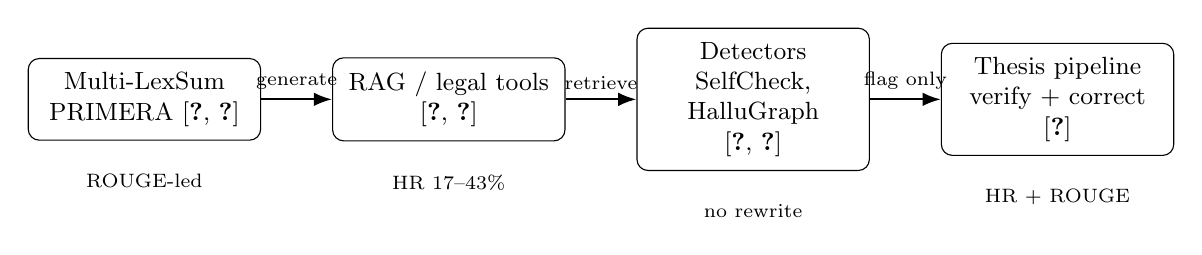
\begin{tikzpicture}[
  font=\small,
  node distance=9mm,
  box/.style={draw, rounded corners, align=center, inner sep=5pt, text width=2.6cm},
  arrow/.style={-Latex, thick}
]
\node[box] (bench) {Multi-LexSum\\PRIMERA \cite{shen2022multilexsum,xiao2022primera}};
\node[box, right=of bench] (rag) {RAG / legal tools\\ \cite{lewis2020rag,magesh2025hallucinationfree}};
\node[box, right=of rag] (detect) {Detectors\\SelfCheck, HalluGraph\\ \cite{manakul2023selfcheckgpt,noel2025hallugraph}};
\node[box, right=of detect] (thesis) {Thesis pipeline\\verify + correct\\ \cite{courtlistener_api}};

\draw[arrow] (bench) -- node[above, font=\scriptsize]{generate} (rag);
\draw[arrow] (rag) -- node[above, font=\scriptsize]{retrieve} (detect);
\draw[arrow] (detect) -- node[above, font=\scriptsize]{flag only} (thesis);

\node[below=3mm of bench, font=\scriptsize, align=center] {ROUGE-led};
\node[below=3mm of rag, font=\scriptsize, align=center] {HR 17--43\%};
\node[below=3mm of detect, font=\scriptsize, align=center] {no rewrite};
\node[below=3mm of thesis, font=\scriptsize, align=center] {HR + ROUGE};
\end{tikzpicture}
\caption{Evolution from benchmark generation (left) to auditable verification and correction (right). Prior work stops at detection or retrieval.}
\label{fig:lit-architecture}
\end{figure}

\subsection{Closing argument for neuro-symbolic legal summarization}

Kautz supplies the \emph{why}; Maynez et al.\ supply the \emph{caution}; Multi-LexSum and Dahl/Magesh supply the \emph{empirical stakes}. Together they justify an architecture that is neither ``bigger LLM'' nor ``better ROUGE,'' but a pipeline where neural fluency is gated by symbolic citation truth. The comparative table in Section~\ref{sec:lit-synthesis} makes this gap explicit across all surveyed papers.

\section{Comparative Synthesis of Surveyed Literature}
\label{sec:lit-synthesis}

Table~\ref{tab:lit-synthesis} consolidates fourteen works (twelve corpus papers plus LEGAL-BERT and Maynez et al.) along dimensions that matter for the thesis: task setting, primary evidence, structural limitation, and the gap relative to verifiable legal summarization.

\begin{table}[!t]
\centering
\caption{Comparative synthesis: evidence, limitations, and thesis gap.}
\label{tab:lit-synthesis}
\small
\begin{tabular}{@{}p{2.5cm}p{2.2cm}p{2.4cm}p{3.8cm}p{3.5cm}@{}}
\toprule
\textbf{Work} & \textbf{Task} & \textbf{Key result} & \textbf{Critical limitation} & \textbf{Thesis gap addressed} \\
\midrule
Multi-LexSum \cite{shen2022multilexsum} & Legal MDS & ROUGE-1 53.73; human faithfulness 0.43/3 & No citation-level verification protocol & HR on CourtListener + correction \\
PRIMERA \cite{xiao2022primera} & MDS & SOTA ROUGE on Multi-LexSum & Optimizes overlap, not citations & Module A + symbolic gate \\
ROUGE \cite{lin2004rouge} & Metric & Correlates on DUC news & Misses factual errors \cite{maynez2020faithfulness} & HR as co-primary metric \\
BERTScore \cite{zhang2020bertscore} & Metric & Better than BLEU on MT & Weak on consistency (TRUE) \cite{honovich2022true} & Joint ROUGE/BERTScore + HR \\
LEGAL-BERT \cite{chalkidis2020legalbert} & Classification & Legal task gains & Not summarization / verification & Optional encoder only \\
Dahl et al.\ \cite{dahl2024largelegalfictions} & Legal QA & 58--88\% HR & Not long summarization & Summarization + taxonomy \\
Magesh et al.\ \cite{magesh2025hallucinationfree} & Tool QA & 17--33\% HR & Closed systems; no correction & Open pipeline + ablations \\
RAG \cite{lewis2020rag} & Open QA & EM 44.5 NQ & No legal citation guarantee & Symbolic post-check \\
HalluGraph \cite{noel2025hallugraph} & Legal QA & AUC 0.84--0.94 & Detection only; preprint & Correction on Multi-LexSum \\
SelfCheckGPT \cite{manakul2023selfcheckgpt} & WikiBio & High AUC-PR & No external legal DB & CourtListener lookup \\
TRUE \cite{honovich2022true} & Meta-metric & NLI/QG best & Not legal citations & Citation-level HR \\
Ji survey \cite{ji2023hallucinationsurvey} & Survey & Mitigation taxonomy & Not operationalized in law & Implemented taxonomy + loop \\
Maynez et al.\ \cite{maynez2020faithfulness} & Summarization & ROUGE--faithfulness gap & General domain & Legal citation focus \\
Pagnoni (FRANK) \cite{pagnoni2021factuality} & Summarization & Factuality taxonomy & No legal DB check & Symbolic verifier \\
Kautz \cite{kautz2022thirdaisummer} & Position & Neuro-symbolic levels & No benchmark & End-to-end legal system \\
\bottomrule
\end{tabular}
\end{table}

\subsection{Cross-cutting themes}

\textbf{Theme 1: Metric decoupling.}
Across Multi-LexSum, Maynez et al., TRUE, and FRANK, automatic scores systematically overestimate usefulness. Any thesis claiming safety must report HR alongside ROUGE/BERTScore.

\textbf{Theme 2: Retrieval $\neq$ verification.}
RAG and commercial legal tools improve grounding but leave double-digit hallucination rates \cite{magesh2025hallucinationfree}. Retrieval supplies evidence; it does not certify citation strings.

\textbf{Theme 3: Detection $\neq$ correction.}
HalluGraph, SelfCheckGPT, and NLI-based metrics flag problems they do not fix. Professional legal workflows need corrected outputs, not only risk scores.

\textbf{Theme 4: Task mismatch.}
Legal QA profiling (Dahl, Magesh, HalluGraph) does not bound summarization risk on 75k-word dockets. Multi-LexSum exposes summarization difficulty but not citation solutions.

\textbf{Theme 5: Auditability.}
Closed commercial systems prevent reproducible science. CourtListener-backed symbolic labels provide per-citation audit trails suitable for error analysis and ablation studies.

\subsection{Positioning statement}

The surveyed literature establishes that legal hallucinations are frequent, that summarization metrics are misleading, and that retrieval and detection help but do not close the accountability loop. No reviewed paper implements \textbf{generate $\rightarrow$ verify $\rightarrow$ correct} for Multi-LexSum summaries with paired case-citation HR against a canonical legal API, including conservative Ambiguous handling and same-case re-anchoring. That unimplemented pipeline is the precise contribution space of this thesis (Chapter~\ref{ch:research-gap} and Chapter~\ref{ch:methodology}).

\paragraph{Implication for dual-system citation verification.}
Related work therefore justifies System~1 (PRIMERA drafts) plus System~2 (eyecite + CourtListener + symbolic correction) as a necessary response to metric decoupling, RAG incompleteness, and detection-without-repair limits, not as an optional post-processing flourish.


\section{Related Work Summary Table}
Table~\ref{tab:relatedwork} summarizes selected related work and the verifiable values used throughout this thesis.

\begin{table}[!t]
\centering
\caption{Verified related work summary (selected).}
\label{tab:relatedwork}
\begin{tabular}{@{}p{3.4cm}p{3.0cm}p{3.0cm}p{4.6cm}@{}}
\toprule
\textbf{Paper} & \textbf{Dataset / Setting} & \textbf{Model / Method} & \textbf{Key result used here (verifiable)} \\
\midrule
Shen et al.\ (Multi-LexSum) \cite{shen2022multilexsum} & Multi-LexSum (legal MDS; long sources) & PRIMERA baseline for \(D \rightarrow L\) & PRIMERA achieves ROUGE-1 53.73, ROUGE-2 27.32, ROUGE-L 30.89 on \(D \rightarrow L\); human rating of generations reported as 0.43 on a 0--3 scale. \\
\addlinespace
Dahl et al.\ \cite{dahl2024largelegalfictions} & Verifiable legal knowledge queries & Multiple public LLMs & Hallucination rates reported between 58\% (ChatGPT-4) and 88\% (Llama 2) on randomly selected federal court cases (task-dependent). \\
\addlinespace
Magesh et al.\ \cite{magesh2025hallucinationfree} & Preregistered evaluation of legal research tools (200+ queries) & Lexis+ AI, Westlaw AI-AR, Ask Practical Law AI & Hallucination rates reported between 17\% and 33\% depending on tool. \\
\addlinespace
No{\"e}l et al.\ (HalluGraph) \cite{noel2025hallugraph} & Legal Contract QA (N=550), Legal Case QA (N=550) & Knowledge-graph alignment metrics & Reported AUC: 0.94 (contracts) and 0.84 (case QA). \\
\addlinespace
Lewis et al.\ (RAG) \cite{lewis2020rag} & Open-domain QA (Natural Questions) & RAG-Sequence / RAG-Token & Natural Questions exact match reported as 44.5 (RAG-Seq) and 44.1 (RAG-Token). \\
\bottomrule
\end{tabular}
\end{table}



\chapter{Research Gap, Questions, and Thesis Objectives}
\label{ch:research-gap}
\section{Research Gap}

Existing approaches expose a core limitation for legal summarization in practice: they can produce fluent summaries but cannot \emph{guarantee} that case citations in the output are correct.
\begin{itemize}
  \item \textbf{Retrieval is not a guarantee.} RAG \cite{lewis2020rag} can improve factuality, but legal evaluations show that even RAG-based tools still hallucinate at non-trivial rates \cite{magesh2025hallucinationfree}.
  \item \textbf{Verification without correction.} Post-hoc detection methods (including structural approaches such as HalluGraph \cite{noel2025hallugraph}) focus on identifying hallucinations, but do not provide an end-to-end Multi-LexSum summarization pipeline that corrects hallucinated citations before output.
  \item \textbf{Missing end-to-end evaluation for summarization.} Legal hallucination profiling \cite{dahl2024largelegalfictions} and legal-tool evaluations \cite{magesh2025hallucinationfree} are not tied to long-document legal summarization with both quality metrics and \emph{paired} citation-faithfulness metrics.
  \item \textbf{Unsafe ``repair'' without identity checks.} Naively replacing a mismatched citation with a database case name can insert an unrelated real case when proprietary identifiers collide, a failure mode this thesis treats as Ambiguous rather than automatic repair.
\end{itemize}

\section{Research Aim and Objectives}

The overall aim of the thesis is:
\begin{quote}
  \emph{To design and evaluate a dual-system, neuro-symbolic pipeline for legal case summarization that verifies and corrects hallucinated case citations, while preserving summarization quality on Multi-LexSum.}
\end{quote}

To achieve this aim, the thesis pursues the following objectives:
\begin{enumerate}
  \item \textbf{Define a case-citation hallucination taxonomy} operationalized as Verified, Mismatch, Ambiguous, NotFound, and Malformed labels against CourtListener.
  \item \textbf{Implement a neural baseline summarizer} (PRIMERA, $D\rightarrow L$) and quantify baseline citation-hallucination behaviour with eyecite extraction.
  \item \textbf{Build a symbolic verifier} that checks extracted citations against CourtListener \cite{courtlistener_api} with auditable explanations.
  \item \textbf{Implement a bounded symbolic correction policy} that redacts unverifiable cites, safely repairs soft mismatches, leaves or re-anchors Ambiguous cites, and never substitutes contradicting CourtListener identities.
  \item \textbf{Evaluate with ablations and statistical testing}, jointly measuring summarization quality (ROUGE-L, optionally BERTScore) and paired draft-citation hallucination rate (HR).
\end{enumerate}

\section{Research Questions}

\begin{itemize}
  \item \textbf{RQ1 (Hallucination measurement):} What types and frequencies of case-citation hallucinations do baseline summarization systems produce on Multi-LexSum under the CourtListener taxonomy?
  \item \textbf{RQ2 (Symbolic verification effectiveness):} Does symbolic verification plus bounded correction measurably reduce \emph{paired} citation hallucination rates compared to a neural-only baseline?
  \item \textbf{RQ3 (Quality preservation under correction):} Can the full dual-system approach (generate $\rightarrow$ verify $\rightarrow$ correct) preserve ROUGE-L\textsubscript{sum} within $\pm 2$ percentage points while reducing paired HR by at least 30\% relative to baseline?
\end{itemize}

\subsection{Consolidated gaps from the literature review}
The literature review (Chapter~\ref{ch:lit-review}) yields five gaps that jointly motivate the thesis design:
\begin{enumerate}
  \item \textbf{Benchmark quality $\neq$ professional reliability.} Multi-LexSum reports moderate ROUGE alongside low human faithfulness for generations \cite{shen2022multilexsum}; overlap metrics do not detect fabricated citations \cite{maynez2020faithfulness,pagnoni2021factuality}.
  \item \textbf{Legal hallucination studies omit long-form summarization.} Dahl et al.\ and Magesh et al.\ quantify hallucinations in QA and tool settings \cite{dahl2024largelegalfictions,magesh2025hallucinationfree}, but not for abstractive multi-document legal summaries with extractable citations.
  \item \textbf{Retrieval and detection without correction.} RAG and detection systems improve or flag factuality but do not rewrite summaries under structured legal-database feedback \cite{lewis2020rag,noel2025hallugraph,manakul2023selfcheckgpt}.
  \item \textbf{Lack of auditable, domain-specific metrics.} General consistency benchmarks (e.g., TRUE) do not replace checking whether a citation exists in a case-law database \cite{honovich2022true}.
  \item \textbf{Neuro-symbolic rhetoric without legal instantiation.} Position papers argue for neuro-symbolic integration \cite{kautz2022thirdaisummer}, but surveyed implementations rarely deliver benchmarked generate--verify--correct pipelines for Multi-LexSum.
\end{enumerate}

\subsection{Proposed evaluation criteria (hypotheses)}
The following success criteria for RQ3 are stated upfront for falsifiability; they are \emph{not} pre-established final results:
\begin{itemize}
  \item \textbf{Citation faithfulness:} relative reduction in paired Hallucination Rate (HR) of at least 30\% versus the neural-only baseline on the evaluated split.
  \item \textbf{Quality preservation:} ROUGE-L\textsubscript{sum} remains within $\pm$2 percentage points of the draft mean (BERTScore reported when enabled).
  \item \textbf{Auditability:} every evaluated summary includes a machine- and human-readable verification/outcome record per draft citation.
\end{itemize}

Pilot citation-rich subsets used during engineering may illustrate trajectories toward these criteria but do not substitute for full-split evaluation.


\chapter{Data Source}
\label{ch:data-source}
\section{Primary Dataset: Multi-LexSum}
\label{sec:data-multilexsum}

This thesis uses Multi-LexSum as the primary benchmark for legal case summarization \cite{shen2022multilexsum}. Multi-LexSum is derived from the Civil Rights Litigation Clearinghouse (CRLC) workflow and provides expert-authored summaries at multiple granularities over long, heterogeneous multi-document sources. The paper reports average source lengths above 75{,}000 words and cases that often exceed 200 pages \cite{shen2022multilexsum}; Chapter~\ref{ch:eda} re-examines these claims on the released Hugging Face layout (one row per case; 4{,}539 cases).

Multi-LexSum provides three target granularities with paper-reported average lengths:
\begin{itemize}
  \item \textbf{Tiny} summaries ($\approx$25 words),
  \item \textbf{Short} summaries ($\approx$130 words),
  \item \textbf{Long} summaries ($\approx$650 words).
\end{itemize}
Exploratory analysis (Chapter~\ref{ch:eda}) shows that long summaries are available for all cases, whereas short and tiny summaries are partially missing. Primary experiments therefore prioritize $D\rightarrow L$.

The dataset is stored locally under \texttt{code/data/} ($\sim$5.9\,GB) and loaded via the project package. Summaries and metadata are released under \textbf{CC BY-NC}; generated audit samples remain internal to coursework per license constraints.

\subsection{Why this corpus}
Multi-LexSum is chosen because it simultaneously stresses (i)~long multi-document abstraction, (ii)~expert reference summaries for ROUGE-style scoring, and (iii)~citation-bearing legal prose in which hallucination is professionally meaningful. Citation recommendation datasets \cite{farber2020citation} answer a different question (suggesting cites) and do not evaluate whether a generated summary invents authorities. Property (iii) is not incidental: Chapter~\ref{ch:eda} measures heuristic case-citation density directly in the expert summaries themselves (Table~\ref{tab:citation-density}) and finds it concentrated almost entirely in the long granularity (1.43 mean citation-like hits per summary, 37.1\% of long summaries containing at least one, versus under 10\% for short and tiny). A corpus where citations were rare or evenly spread across granularities would not support a citation-faithfulness study at any useful scale; Multi-LexSum's long summaries are citation-dense enough that a fixed evaluation subset can be drawn specifically for citation richness (Section~\ref{sec:eval-case-selection}).

\subsection{Case selection for evaluation}
\label{sec:eval-case-selection}
Full-scale evaluation (Chapter~\ref{ch:evaluation-method}) does not sample uniformly at random from the test split. Because paired HR is only informative on cases that actually contain citations to hallucinate or verify, the evaluation set is the 100 test-split cases with the highest heuristic citation density (the same regex proxy used for Table~\ref{tab:citation-density}), fixed once and reused identically across all three Module~A generators (Section~\ref{sec:module-a-crossmodel}) so that generator comparisons are not confounded by different case sets. This is a deliberate stress test, not a claim of representativeness: it reports how the pipeline performs where citations are dense, which is also where a hallucination is most likely and most consequential, rather than an unconditional average over cases that may contain no checkable citations at all.

\section{External Verification Resource: CourtListener}
\label{sec:data-courtlistener}

The symbolic verifier uses the \textbf{CourtListener API} operated by the Free Law Project for U.S.\ case-law citation lookup \cite{courtlistener_api,freelawproject}. Citation strings are extracted with eyecite \cite{eyecite2021} before lookup. This stack is preferred over closed commercial oracles because it supports reproducible science, per-citation explanations, and offline caching under documented rate limits: concretely, the evaluation account's confirmed access level of 10 requests/minute, 100/hour, and 250/day (Section~\ref{sec:module-c}), which the implementation treats as a hard operating constraint rather than a soft target.

\section{Manually Labeled Audit Subset}
\label{sec:audit-subset}

To support hallucination measurement and error analysis, a stratified subset of 200 generated summaries, drawn from the validation and test splits and seeded for reproducibility, is reserved for manual review to (i)~validate extraction behaviour and (ii)~spot-check automated labels (fabricated cites vs.\ soft mismatches vs.\ Ambiguous identity clashes). The EDA pipeline exports \texttt{sample\_indices.csv} for reproducible stratified sampling, and the evaluation harness separately exports a manual-labelling template for this 200-case pool. Automated RQ answers remain distinct from manual audit labels; the audit is a validity check on the automated taxonomy, not an input to RQ1--RQ3 scoring.

\section{Connection to Exploratory Analysis and Methodology}
\label{sec:data-bridge}

Chapter~\ref{ch:eda} quantifies corpus shape, truncation risk, and citation density that motivate $D\rightarrow L$ and untrusted drafts. Chapter~\ref{ch:methodology} then specifies how Multi-LexSum inputs and CourtListener responses are wired into Modules~A--C and the correction loop.


\chapter{Exploratory Data Analysis}
\label{ch:eda}
\section{Objectives and Method}
\label{sec:eda-objectives}

Before trusting any neural summarizer or citation verifier, this thesis asks what Multi-LexSum \emph{actually} contains. The exploratory data analysis (EDA) is implemented in \texttt{notebooks/multilexsum\_eda.ipynb} and writes reproducible tables to \texttt{code/reports/tables/} and figures to \texttt{Documentation/figures/eda/}. The analysis addresses five practical questions:
\begin{enumerate}
  \item How are cases distributed across splits, and which summary granularities are available per case?
  \item How do expert summary lengths compare to the paper's target word counts?
  \item How long and heterogeneous are multi-document sources, and what fraction exceeds common model context budgets?
  \item What civil-rights case types and filing years does the benchmark cover?
  \item How densely do expert summaries contain case-citation patterns at each granularity, motivating the symbolic verification module?
\end{enumerate}

All statistics below are computed on \textbf{4{,}539 cases} (train: 3{,}177; validation: 454; test: 908), matching the Hugging Face release structure of one row per case with up to three summary fields. Each figure is interpreted in three steps: \emph{what it shows}, \emph{what it implies}, and \emph{how it changes system design}.

\section{Corpus Shape and Summary Availability}
\label{sec:eda-corpus-shape}

Table~\ref{tab:split-inventory} confirms the standard Multi-LexSum split sizes. Unlike the paper's count of 9{,}280 \emph{summary instances}, the released dataset stores one record per case; long summaries are present for every case, while short and tiny summaries are partially missing.

\begin{table}[!t]
\centering
\caption{Multi-LexSum split inventory (cases per split).}
\label{tab:split-inventory}
\begin{tabular}{@{}l r@{}}
\toprule
\textbf{Split} & \textbf{Cases} \\
\midrule
Train      & 3{,}177 \\
Validation & 454 \\
Test       & 908 \\
\midrule
\textbf{Total} & \textbf{4{,}539} \\
\bottomrule
\end{tabular}
\end{table}

Long summaries (\texttt{summary/long}) are present for 100\% of cases in every split. Short summaries are present for 69.6\% (train), 68.7\% (validation), and 67.8\% (test). Tiny summaries are present for only 35.6\%, 35.5\%, and 34.4\%, respectively.

\begin{figure}[!t]
\centering
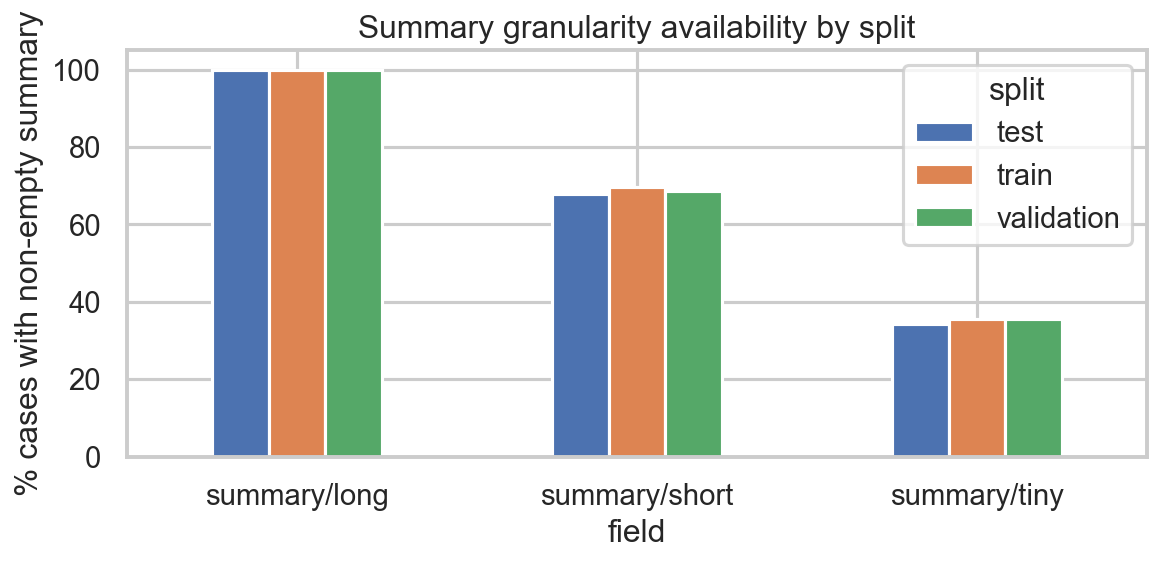
\includegraphics[width=0.92\linewidth]{summary_availability.png}
\caption{Percentage of cases with a non-empty expert summary at each granularity, by split. Long summaries form a complete bar at 100\%; short and tiny bars fall substantially lower.}
\label{fig:summary-availability}
\end{figure}

\paragraph{Reading Figure~\ref{fig:summary-availability}.}
The plot compares three granularities across train/validation/test. The dominant visual signal is the unbroken 100\% availability of long summaries contrasted with partial short coverage and sparse tiny coverage. The pattern is stable across splits, which indicates a dataset design property rather than a split-specific corruption.

\paragraph{Design implication.}
Tasks $D\rightarrow S$ and especially $D\rightarrow T$ have fewer supervised targets than $D\rightarrow L$. Primary summarization and citation-verification experiments therefore prioritize document-to-long summarization.

\section{Summary Length Distributions}
\label{sec:eda-summary-lengths}

Table~\ref{tab:summary-word-stats} compares empirical word-count statistics on the test split to the paper's target averages (650 / 130 / 25 words). Median long-summary length (407 words) is below the 650-word target but within the same order of magnitude; short and tiny medians (97 and 19 words) track the paper targets closely.

\begin{table}[!t]
\centering
\caption{Expert summary word-count statistics on the test split (present summaries only).}
\label{tab:summary-word-stats}
\begin{tabular}{@{}l r r r r@{}}
\toprule
\textbf{Field} & \textbf{$n$} & \textbf{Mean} & \textbf{Median} & \textbf{Paper target} \\
\midrule
\texttt{summary/long}  & 908 & 521.3 & 407.0 & 650 \\
\texttt{summary/short} & 616 & 111.4 & 97.0  & 130 \\
\texttt{summary/tiny}  & 312 & 21.6  & 19.0  & 25  \\
\bottomrule
\end{tabular}
\end{table}

\begin{figure}[!t]
\centering
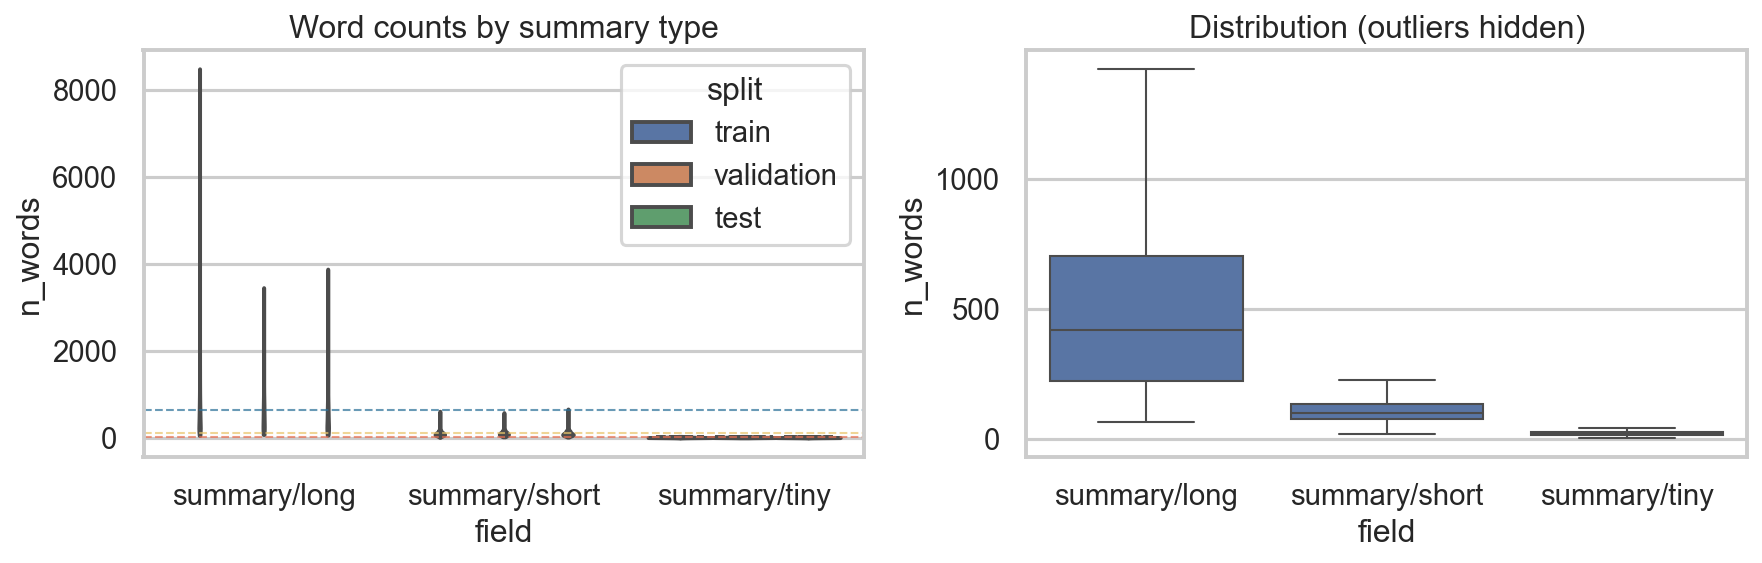
\includegraphics[width=\linewidth]{summary_words_violin.png}
\caption{Expert summary word counts by granularity and split (left: violin with targets as dashed lines; right: boxplot with outliers hidden).}
\label{fig:summary-words}
\end{figure}

\paragraph{Reading Figure~\ref{fig:summary-words}.}
The left panel shows wide long-summary distributions with a heavy right tail (test maximum 3{,}883 words), while short and tiny clusters near their dashed target lines. The right panel confirms that central mass for long summaries sits below the 650-word target even after hiding outliers. Splits behave similarly, so length skew is corpus-wide.

\paragraph{Design implication.}
ROUGE evaluation against long references remains meaningful, but systems should not be judged solely by matching a nominal 650-word average. Extreme long targets also increase the opportunity for citation-bearing sentences, relevant to Module~B.

\section{Granularity Switching and Compression}
\label{sec:eda-granularity}

Switching the target granularity changes both usable-case counts and compression ratio (source words / summary words). On the training split, median compression for long summaries is approximately 58$\times$, compared with roughly 2{,}400$\times$ for tiny summaries.

\begin{figure}[!t]
\centering
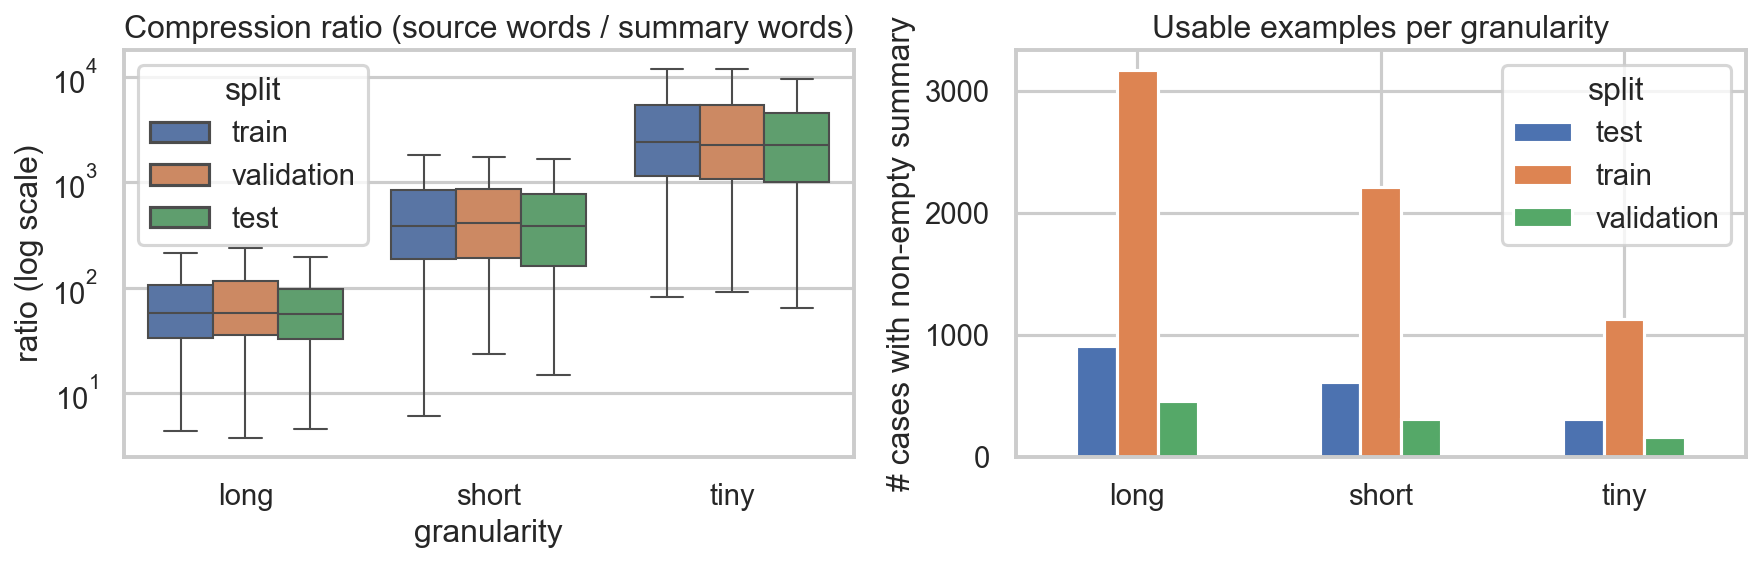
\includegraphics[width=\linewidth]{granularity_switch_analysis.png}
\caption{Left: compression ratio by granularity (log scale). Right: count of cases with non-empty expert summaries.}
\label{fig:granularity-switch}
\end{figure}

\paragraph{Reading Figure~\ref{fig:granularity-switch}.}
The left panel's log-scale boxes rise sharply from long to tiny, visualizing how aggressively each output word must compress the docket. The right panel restates availability: long bars dominate usable supervision. Together, the panels show that ``harder compression'' and ``fewer labels'' coincide at tiny granularity.

\paragraph{Design implication.}
Long summaries offer the richest context for citation extraction and verification; tiny summaries compress so aggressively that both modelling and citation auditing become less informative. This supports prioritizing $D\rightarrow L$ for RQ1--RQ3.

\section{Multi-Document Source Structure}
\label{sec:eda-sources}

Each case concatenates multiple legal documents. Corpus-wide source statistics are summarized in Table~\ref{tab:source-stats}. Mean source length (61{,}539 words) is consistent with the Multi-LexSum paper's long-docket narrative; the median (24{,}546 words) is lower, reflecting a heavy-tailed distribution.

\begin{table}[!t]
\centering
\caption{Per-case source statistics (all splits combined, $n=4{,}539$).}
\label{tab:source-stats}
\begin{tabular}{@{}l r r r@{}}
\toprule
\textbf{Statistic} & \textbf{Mean} & \textbf{Median} & \textbf{95th percentile} \\
\midrule
Source words        & 61{,}539 & 24{,}546 & 226{,}408 \\
Source characters   & 399{,}409 & 158{,}734 & 1{,}475{,}231 \\
\# source documents & 8.8 & 6.0 & 26.0 \\
\bottomrule
\end{tabular}
\end{table}

Approximately 35.1\% of cases include at least one OCR-derived source document.

\begin{figure}[!t]
\centering
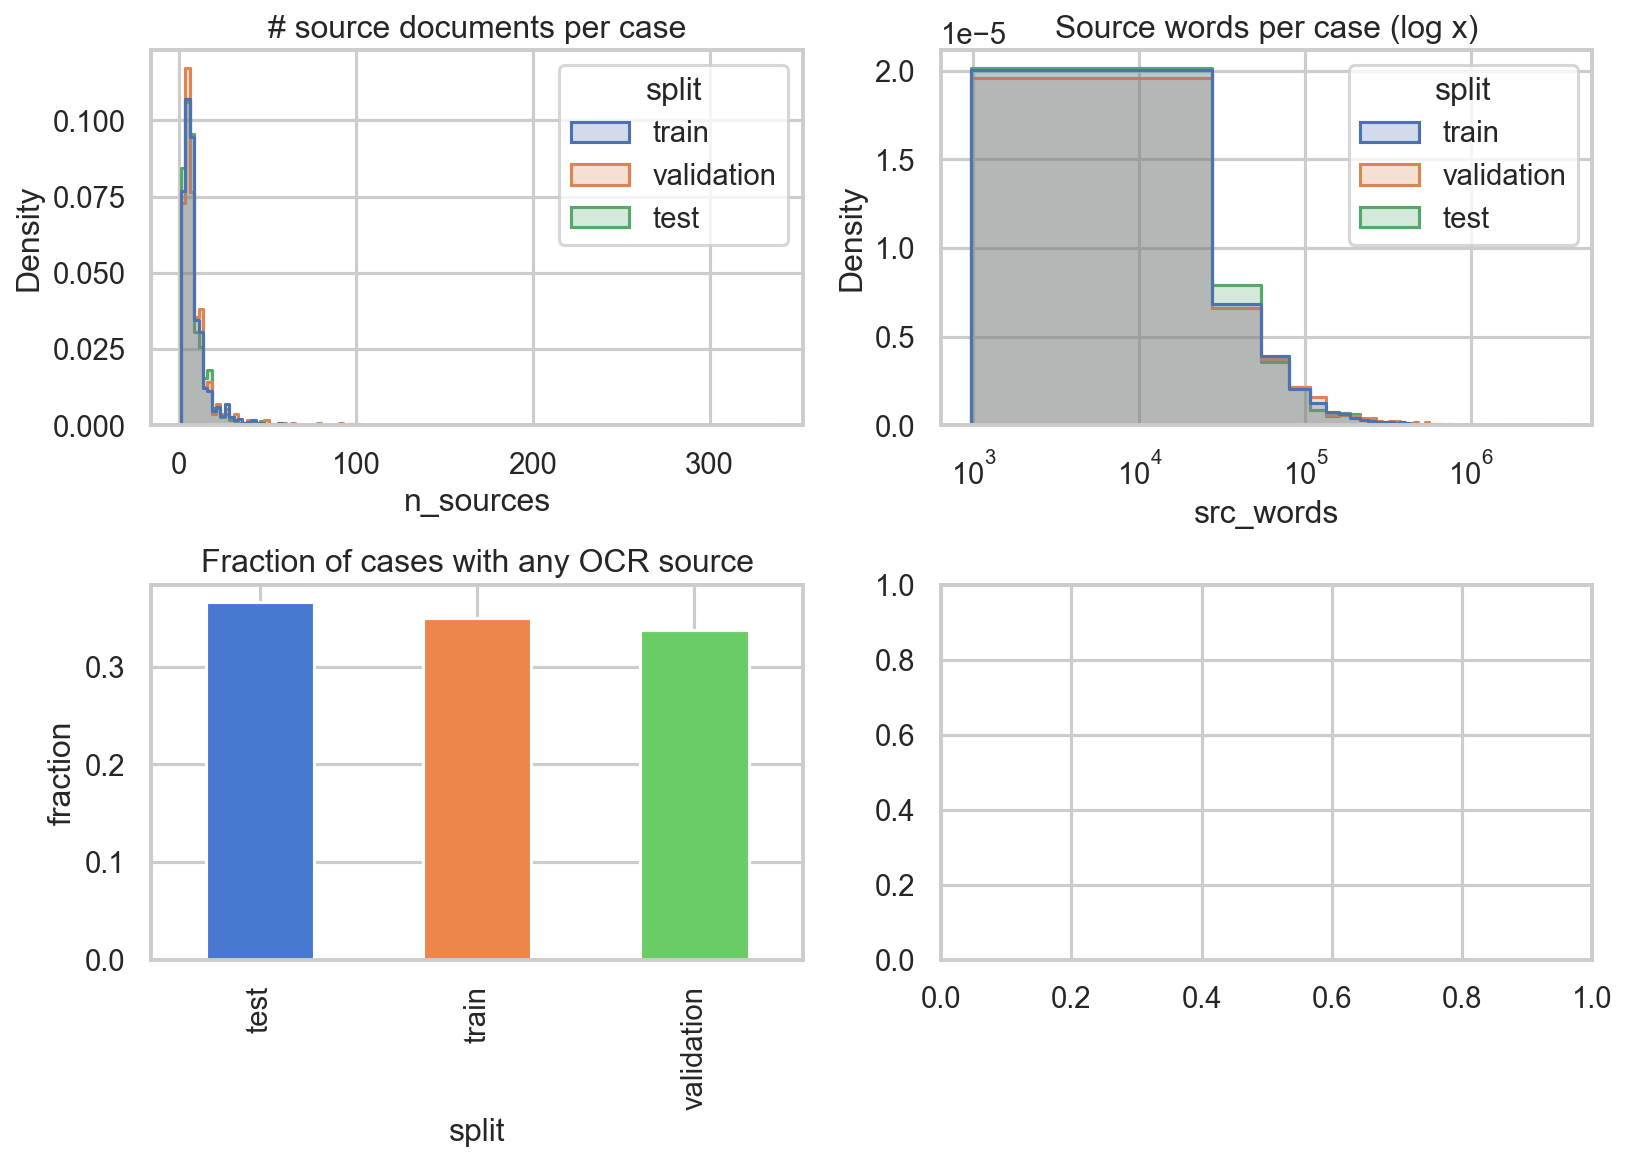
\includegraphics[width=0.88\linewidth]{source_distributions.png}
\caption{Per-case source document count (top left) and source word count on a log scale (top right). Bottom left: fraction of cases with any OCR source by split.}
\label{fig:source-distributions}
\end{figure}

\paragraph{Reading Figure~\ref{fig:source-distributions}.}
Document-count histograms peak at modest multi-document bundles but exhibit a long tail. Source-word histograms on a log axis show that ``typical'' cases are already tens of thousands of words, while a minority explode toward $10^5$--$10^6$ words. OCR prevalence near one-third warns that noisy text is common rather than exceptional.

\paragraph{Design implication.}
Module~A must assume heterogeneous, multi-file inputs. OCR noise can break brittle string matching, which is one reason Module~C reports Ambiguous/NotFound rather than forcing a match.

\section{Truncation Risk Under Fixed Context Budgets}
\label{sec:eda-truncation}

A GPT-2 tokenizer audit measures what fraction of cases exceed common token budgets (Table~\ref{tab:truncation}; training split).

\begin{table}[!t]
\centering
\caption{Fraction of training cases whose concatenated sources exceed a GPT-2 token budget.}
\label{tab:truncation}
\begin{tabular}{@{}r r@{}}
\toprule
\textbf{Token budget} & \textbf{Fraction exceeding} \\
\midrule
2{,}048    & 100.0\% \\
4{,}096    & 99.4\% \\
8{,}192    & 91.8\% \\
32{,}768   & 57.8\% \\
65{,}536   & 38.9\% \\
131{,}072  & 14.4\% \\
\bottomrule
\end{tabular}
\end{table}

\begin{figure}[!t]
\centering
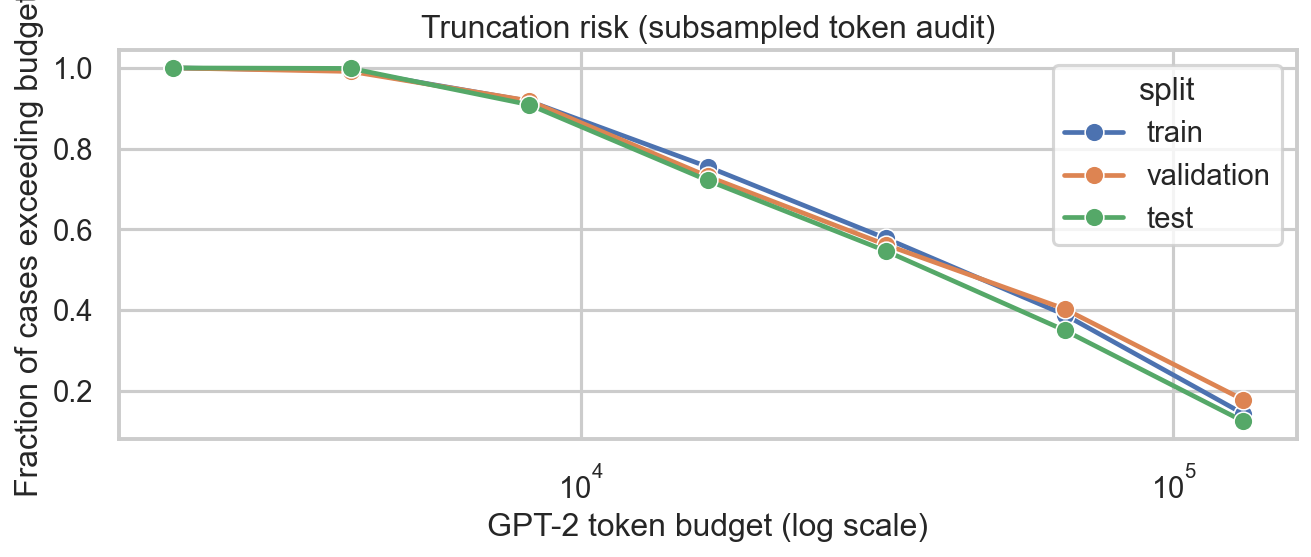
\includegraphics[width=0.88\linewidth]{truncation_fractions.png}
\caption{Fraction of cases exceeding a GPT-2 token budget across splits (log-scaled budgets on the $x$-axis).}
\label{fig:truncation}
\end{figure}

\paragraph{Reading Figure~\ref{fig:truncation}.}
All splits decay similarly: almost every case exceeds small budgets; a majority still exceed 32k tokens; a non-trivial fraction remains over budget even at 131k. The curve is the empirical argument against pretending Module~A ``reads the whole case.''

\paragraph{Design implication.}
Faithful summarization and citation verification must assume partial observability of the source. The dual-system design therefore treats the neural summarizer as an untrusted draft generator whose outputs are audited symbolically \cite{maynez2020faithfulness,beltagy2020longformer}. The 4{,}096-token truncation used for the full-scale run is an explicit, documented constraint, not a hidden footnote.

\section{Case Types, Outcomes, and Filing Years}
\label{sec:eda-metadata}

Multi-LexSum cases are drawn from U.S.\ civil-rights litigation filed between 1951 and 2021. The most frequent case type is Equal Employment (1{,}579 cases), followed by Immigration and/or the Border (523) and Prison Conditions (424). Plaintiffs prevail in 3{,}143 cases; defendants in 564; outcomes are mixed or pending for the remainder. Class actions are sought in 1{,}510 cases (33.3\%).

\begin{figure}[!t]
\centering
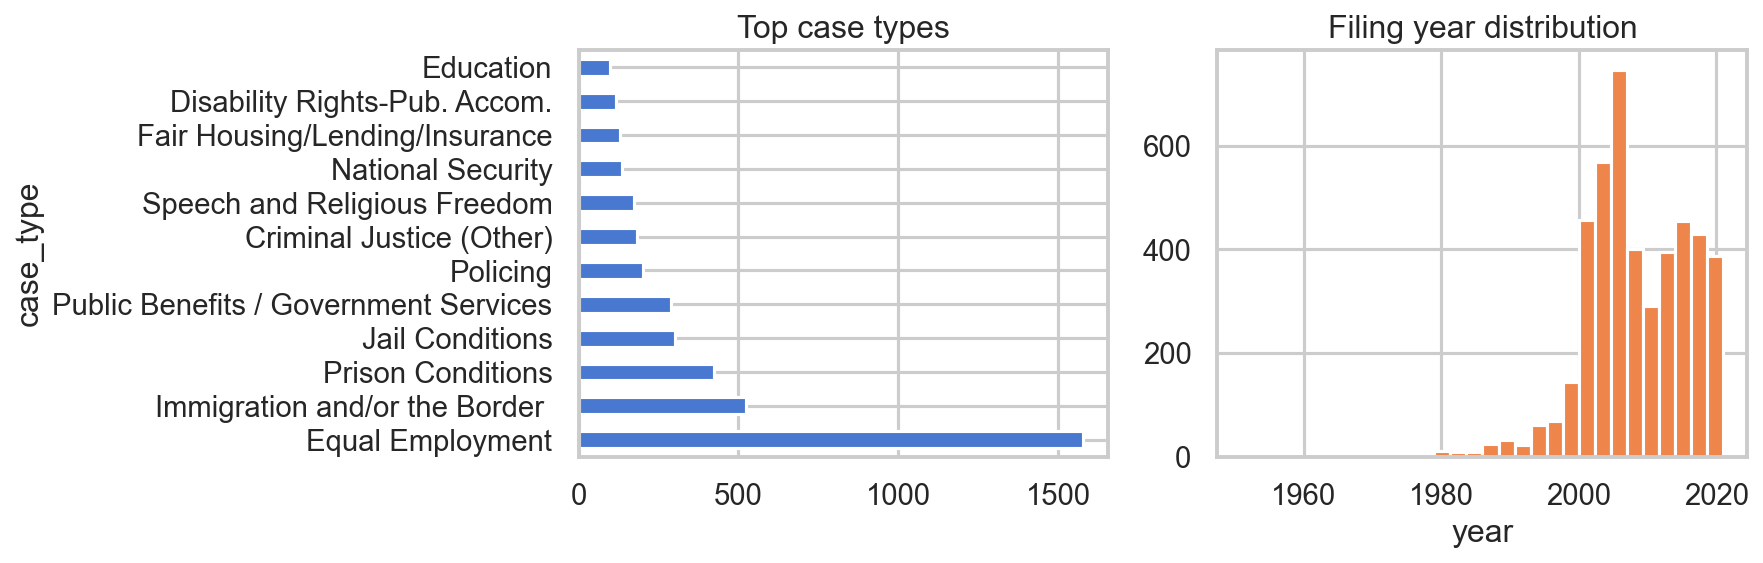
\includegraphics[width=\linewidth]{metadata_landscape.png}
\caption{Top case types (left) and filing-year distribution (right).}
\label{fig:metadata}
\end{figure}

\paragraph{Reading Figure~\ref{fig:metadata}.}
The left panel shows a skewed case-type distribution dominated by employment litigation, with a long tail of other civil-rights categories. The right panel shows filings spanning seven decades, concentrated in more recent decades but not confined to a single era. Domain diversity is real, but not uniform.

\paragraph{Design implication.}
Citation verification must handle heterogeneous reporters and eras. A single ``easy'' subset (e.g., only modern Supreme Court cites) would overstate verifier performance.

\section{Citation Density in Expert Summaries}
\label{sec:eda-citations}

Expert summaries provide a proxy for where citations appear in gold text. Regex heuristics (Federal Reporter patterns, \texttt{v.} party pairs) extract candidate spans, noisy but useful for relative comparisons across granularities.

\begin{table}[!t]
\centering
\caption{Heuristic citation statistics in expert summaries (train split, present summaries only).}
\label{tab:citation-density}
\begin{tabular}{@{}l r r r@{}}
\toprule
\textbf{Granularity} & \textbf{Mean hits} & \textbf{\% with $\geq 1$ hit} & \textbf{Mean cites / 100 words} \\
\midrule
Long  & 1.43 & 37.1\% & 0.20 \\
Short & 0.10 & 7.6\%  & 0.07 \\
Tiny  & 0.02 & 2.1\%  & 0.12 \\
\bottomrule
\end{tabular}
\end{table}

\begin{figure}[!t]
\centering
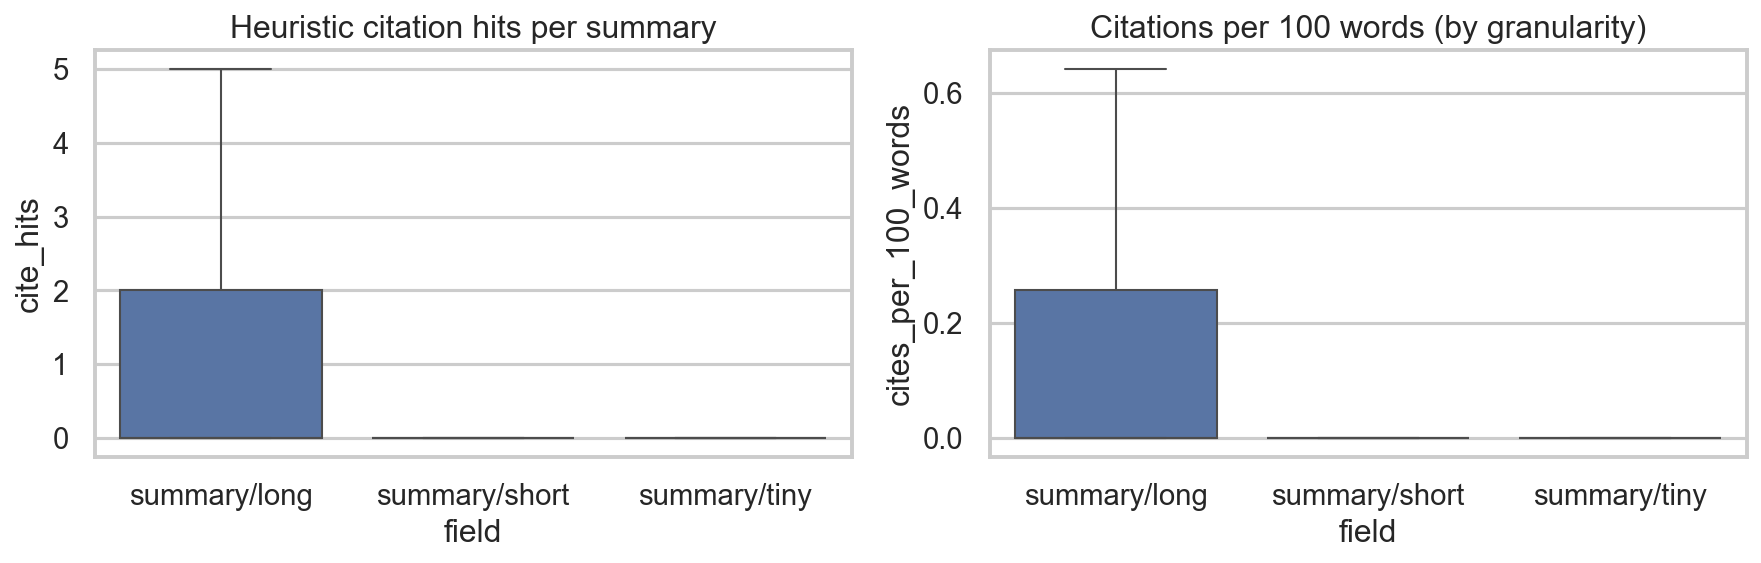
\includegraphics[width=\linewidth]{citation_by_granularity.png}
\caption{Heuristic citation hits (left) and citations per 100 words (right) by summary granularity.}
\label{fig:citation-granularity}
\end{figure}

\paragraph{Reading Figure~\ref{fig:citation-granularity}.}
Long summaries dominate absolute hit counts: most mass sits at zero, but the upper quartile carries multiple hits. Short and tiny summaries rarely contain heuristic cites. Normalized density (right) remains highest for long targets in absolute opportunity for Module~B, even though per-100-word rates can look noisy at tiny lengths due to short denominators.

\paragraph{Design implication.}
Citation verification is most informative at the long granularity. Module~B therefore targets $D\rightarrow L$ outputs; regex EDA is only a prior, and production extraction uses eyecite \cite{eyecite2021}.

\section{Data Quality Checks}
\label{sec:eda-quality}

Automated anomaly checks found no empty long summaries, no empty source lists, and no zero-length source documents. Missing short and tiny summaries are dataset characteristics rather than corruption (Section~\ref{sec:eda-corpus-shape}). The EDA pipeline exports \texttt{sample\_indices.csv} for stratified manual review; per license constraints, raw summary text from the audit subset remains internal to coursework.

\section{Summary of EDA Findings}
\label{sec:eda-summary}

The EDA supports four design decisions for the remainder of the thesis:
\begin{enumerate}
  \item \textbf{Primary task:} $D\rightarrow L$, where all splits have complete labels and citation opportunity is highest.
  \item \textbf{Modeling constraint:} truncation/chunking is unavoidable for most cases; faithfulness cannot rely on full-source attention alone.
  \item \textbf{Verification focus:} case-citation checking targets long outputs; short/tiny ablations are secondary.
  \item \textbf{Baseline expectations:} expert summaries already show moderate deviation from nominal length targets and sparse citation patterns under regex mining; automatic systems face a difficult faithfulness ceiling even before hallucination is measured on model outputs.
\end{enumerate}

These findings do not yet answer RQ1--RQ3, which require generated summaries from Module~A. They establish the empirical context in which the dual-system pipeline of Chapter~\ref{ch:methodology} is designed.


\chapter{Methodology: Methods, Tools, and Technologies}
\label{ch:methodology}
\section{Research Design and Narrative Overview}
\label{sec:method-design}

This thesis follows a \textbf{design--implement--evaluate} methodology. Chapter~\ref{ch:eda} established what the Multi-LexSum corpus looks like in practice and which modelling assumptions are unsafe (complete short/tiny coverage; full-document encoding). The present chapter translates those findings into an implemented dual-system pipeline, in the sense used throughout this thesis: a fast, pattern-matching neural component (\textbf{System~1}) that drafts fluent text without any guarantee that its claims are checkable, paired with a slower, rule-governed component (\textbf{System~2}) that audits a specific, well-defined class of those claims, case citations, against an external source of truth. The terminology follows Kahneman's dual-process account of fast, associative versus slow, deliberative reasoning \cite{kahneman2011thinkingbook}, as adapted to system design by neuro-symbolic AI arguments that System~1 (neural) outputs need System~2 (symbolic, deliberative) checks in domains where an unchecked error carries professional or safety consequences \cite{kautz2022thirdaisummer}. Concretely, System~1 is Module~A (Section~\ref{sec:module-a}); System~2 is Modules~B and~C plus the bounded correction policy (Sections~\ref{sec:module-b}--\ref{sec:correction}).

The design is deliberately \emph{asymmetric}. Neural models remain responsible for fluent multi-document abstraction, a task where they excel \cite{xiao2022primera,shen2022multilexsum}. They are \emph{not} trusted as the final authority on whether a case citation exists. That authority is delegated to an auditable symbolic layer backed by CourtListener \cite{courtlistener_api,eyecite2021}, consistent with the System~1/System~2 division above: System~1 is never asked to self-certify a claim it has no mechanism to verify.

\begin{enumerate}
  \item \textbf{Baseline generation.} Produce long ($D\rightarrow L$) draft summaries with PRIMERA under an explicit truncation budget motivated by Chapter~\ref{ch:eda}.
  \item \textbf{Citation extraction and verification.} Extract \texttt{FullCaseCitation} spans with eyecite; verify each span against CourtListener; assign Verified / Mismatch / Ambiguous / NotFound / Malformed labels.
  \item \textbf{Bounded correction.} Redact unverifiable cites; safely repair soft mismatches; leave or \emph{re-anchor} Ambiguous cites; never substitute a contradicting CourtListener case name.
  \item \textbf{Paired evaluation.} Track each draft citation through correction using stable \texttt{citation\_id}s; report paired hallucination rate (HR) jointly with ROUGE-L.
\end{enumerate}

A preliminary citation-rich validation subset ($n=10$) is used during development to stress-test labelling and correction policies. Those numbers are reported as \textbf{pilot evidence} only; they do not replace a full validation/test evaluation in later chapters.

\section{End-to-End Architecture}
\label{sec:method-architecture}

Figure~\ref{fig:architecture} shows the implemented pipeline. Relative to earlier design sketches that assumed free-form LLM regeneration of the entire summary, the correction stage is now primarily \textbf{symbolic} (span redact / replace / re-anchor), with an optional light LLM rewrite path that must re-verify.

\begin{figure}[!t]
\centering
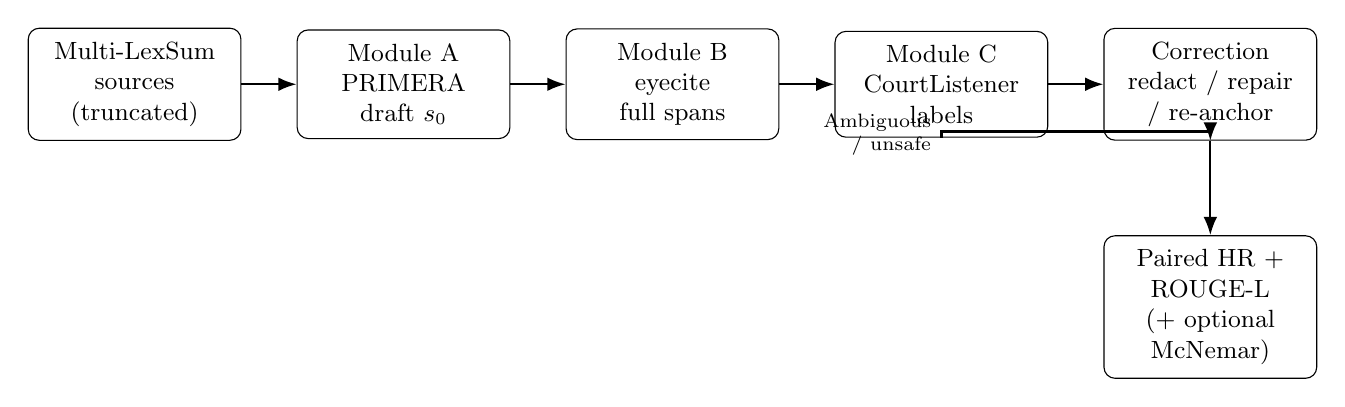
\begin{tikzpicture}[
  font=\small,
  node distance=9mm and 7mm,
  box/.style={draw, rounded corners, align=center, inner sep=5pt, text width=2.35cm},
  arrow/.style={-Latex, thick}
]
\node[box] (input) {Multi-LexSum\\sources\\(truncated)};
\node[box, right=of input] (summ) {Module A\\PRIMERA\\draft $s_0$};
\node[box, right=of summ] (extract) {Module B\\eyecite\\full spans};
\node[box, right=of extract] (verify) {Module C\\CourtListener\\labels};
\node[box, right=of verify] (corr) {Correction\\redact / repair\\/ re-anchor};
\node[box, below=12mm of corr] (eval) {Paired HR + ROUGE-L\\(+ optional McNemar)};

\draw[arrow] (input) -- (summ);
\draw[arrow] (summ) -- (extract);
\draw[arrow] (extract) -- (verify);
\draw[arrow] (verify) -- (corr);
\draw[arrow] (corr) -- (eval);
\draw[arrow] (verify) -- node[left, align=right, font=\scriptsize]{Ambiguous\\/ unsafe} ++(0,-6mm) -| (corr);
\end{tikzpicture}
\caption{Dual-system architecture as implemented: neural draft generation followed by symbolic citation verification and bounded correction. Evaluation tracks draft citations through correction (paired HR).}
\label{fig:architecture}
\end{figure}

\section{Module A: Neural Summarization}
\label{sec:module-a}

\subsection{Why PRIMERA}
Module~A uses PRIMERA \cite{xiao2022primera}, a multi-document summarization model that is a strong Multi-LexSum baseline \cite{shen2022multilexsum}. The choice is pragmatic and scientific: (i)~it matches the benchmark setting against which ROUGE improvements are usually claimed; (ii)~it forces the thesis to confront citation faithfulness on a realistic neural draft rather than on toy extractive baselines.

\subsection{Why $D\rightarrow L$ only}
Chapter~\ref{ch:eda} showed that long summaries are complete for every case, while short and tiny fields are systematically missing, and that heuristic citation density is highest in long targets. Primary experiments therefore use document-to-long ($D\rightarrow L$) summarization. Short/tiny settings remain available for future ablation, not for the core RQ answers.

\subsection{Truncation policy}
EDA demonstrated that more than 90\% of training cases exceed an 8{,}192-token budget and that even 131k-token budgets leave a non-trivial residue. Module~A therefore applies an explicit \textbf{naive truncation} to a fixed token budget (4{,}096 tokens, the architectural ceiling of the PRIMERA checkpoint used for the full-scale run, confirmed from its \texttt{max\_encoder\_position\_embeddings}, not a demo-time simplification). This is an honest operating constraint, not a claim of optimal long-context modelling. The dual-system thesis \emph{depends} on this honesty: if the model cannot see the full docket, symbolic verification of citations becomes more important, not less \cite{maynez2020faithfulness,beltagy2020longformer}.

\subsection{Generation length calibration}
Full-scale generation initially produced summaries well short of the $D\rightarrow L$ target (mean 461 words against an $\approx$850-token/650-word budget). Inspection traced this to the PRIMERA checkpoint's own \texttt{generation\_config.json}, which ships \texttt{length\_penalty=0}: with no length normalization, beam search scores candidates by raw summed log-probability, which mathematically favours shorter sequences, since every additional token multiplies in a probability $\le 1$. Nothing in the pipeline overrode this default. Module~A now sets an explicit \texttt{min\_new\_tokens} floor and \texttt{length\_penalty=2.0}, raising mean length to 535 words. This is reported as a calibration decision, not a result: it establishes that the citation-attempt comparisons across generators in Section~\ref{sec:module-a-crossmodel} reflect genuine generation behaviour rather than an unexamined default.

Listing~\ref{lst:module-a-generate} shows the calibrated call as implemented: the explicit \texttt{min\_new\_tokens} and \texttt{length\_penalty} arguments are the fix, not defaults inherited from the checkpoint.

\begin{lstlisting}[caption={Module~A batch generation call with the length-calibration fix explicit (\href{\repourl/blob/main/src/module_a_summarizer/generate.py}{\texttt{src/module\_a\_summarizer/generate.py}}).}, label={lst:module-a-generate}]
max_new_tokens = config["max_new_tokens"][granularity]
min_new_tokens = config.get("min_new_tokens", {}).get(granularity)
length_penalty = config.get("length_penalty", 2.0)  # overrides checkpoint's 0
num_beams = config.get("num_beams", 5)

for case in pending:
    generated = summarizer.generate(
        case.sources_text,
        max_new_tokens=max_new_tokens,
        num_beams=num_beams,
        min_new_tokens=min_new_tokens,
        length_penalty=length_penalty,
        early_stopping=early_stopping,
    )
    _append_row(out_path, {"case_id": case.case_id, "generated_summary": generated, ...})
\end{lstlisting}

\subsection{Cross-model comparison: LLM and LLM+retrieval variants}
\label{sec:module-a-crossmodel}

Development-time inspection of full-scale PRIMERA drafts showed markedly fewer attempted case citations than the corresponding expert summaries on the same citation-dense cases, an observation that motivates, rather than answers, a question this thesis is positioned to test: is low citation-attempt density a property of neural legal summarization in general, or an artefact of one checkpoint's output-length ceiling and truncation window? To probe this, Module~A is extended with two further generators evaluated on the identical case set:

\begin{itemize}
  \item \textbf{LLM zero-shot.} Qwen2.5-7B-Instruct \cite{qwen2025qwen25,yang2024qwen2}, an instruction-tuned open-weight model (Apache-2.0), given an 8{,}192-token input budget (double PRIMERA's architecturally fixed 4{,}096 above) and an explicit instruction to preserve every real case citation present in the source material, with an approximately 2{,}000-token output budget.
  \item \textbf{LLM + retrieval.} The same checkpoint and budgets, but source documents are ranked by a fast citation-density heuristic before truncation, rather than kept in naive chronological order. Ranking uses a regex proxy for citation-like patterns rather than a full eyecite parse: eyecite's cross-reference resolution over the full, untruncated source text of 100 dockets (some exceeding 100{,}000 tokens each) is not fast enough to justify for what is only a coarse relevance signal, and precise extraction downstream (Module~B) is unaffected by this choice. This variant operationalizes, for the first time inside this pipeline rather than by citation to prior work, the retrieval-versus-symbolic-verification distinction the literature review raises (Section~\ref{sec:lit-rag}, Table~\ref{tab:rag-vs-symbolic}).
\end{itemize}

Both variants are evaluated under the same generate--verify--correct pipeline (Sections~\ref{sec:module-b}--\ref{sec:correction}) and the same four conditions (Section~\ref{sec:conditions}) as the PRIMERA baseline, producing a $3\times4$ generator--condition matrix. Comparative citation-attempt counts, hallucination rates, and quality metrics across the three generators are reported in the results chapter once full-scale verification of all three completes.

\section{Module B: Case Citation Extraction}
\label{sec:module-b}

Module~B uses eyecite \cite{eyecite2021} to extract \texttt{FullCaseCitation} objects from draft text. Three implementation details are central to evaluation integrity:

\begin{itemize}
  \item \textbf{Full spans.} Replacements operate on the full citation span (including party names when present), not only the reporter substring. Reporter-only edits historically produced garbled hybrids (case name spliced into a reporter fragment).
  \item \textbf{Stable \texttt{citation\_id}.} Each extracted citation receives an identifier derived from normalized cite text and character offsets, enabling paired tracking from draft to corrected summary.
  \item \textbf{Markup sanitization.} Multi-LexSum source documents retain HTML markup from their originating court-record/Clearinghouse pages (e.g.\ \texttt{<i>Obergefell v.\ Hodges</i>}), which extractive-leaning PRIMERA drafts can copy verbatim; LLM-generated drafts introduce analogous Markdown emphasis (\texttt{**Graham**}). Either corrupts eyecite's antecedent/party-name guessing when markup sits directly adjacent to a case name, observed directly in development runs and traced to malformed \texttt{party\_names} extraction (e.g.\ \texttt{("", "Hodges</i>")} instead of \texttt{("Obergefell", "Hodges")}) that propagated into an incorrect correction-loop outcome for an otherwise real, correctly identifiable citation. Extraction now blanks HTML tags and Markdown emphasis markers with equal-length whitespace before parsing, length-preserving, so citation-span character offsets used elsewhere for redaction and replacement remain valid against the original text.
\end{itemize}

Listing~\ref{lst:module-b-blank} shows the markup-blanking fix: tags and Markdown emphasis are replaced with equal-length whitespace, not deleted, so every downstream character offset used for redaction or replacement still lines up with the original text.

\begin{lstlisting}[caption={Length-preserving markup blanking before eyecite parsing (\href{\repourl/blob/main/src/module_b_extraction/extract_citations.py}{\texttt{src/module\_b\_extraction/extract\_citations.py}}).}, label={lst:module-b-blank}]
_MARKUP_RE = re.compile(r"</?i>|</?b>|</?em>|</?strong>|\*\*|<a\s[^>]*>|</a>")

def _blank_markup(text: str) -> str:
    return _MARKUP_RE.sub(lambda m: " " * len(m.group()), text)

def extract_citations(summary_text: str) -> list[ExtractedCitation]:
    cleaned_text = _blank_markup(summary_text)
    results = []
    for c in get_citations(cleaned_text):
        if not isinstance(c, FullCaseCitation):
            continue
        results.append(ExtractedCitation(
            raw_text=c.corrected_citation_full(),
            normalized=str(c.corrected_citation()),
            party_names=_party_names_from_citation(c),
            span=_full_span_from_citation(c),
            citation_id=make_citation_id(...),
        ))
    return results
\end{lstlisting}

Extraction is deliberately narrower than ``any legal reference'': pin cites and some proprietary identifiers are handled as attributes of a full case citation when eyecite exposes them. This reduces false positives in hallucination accounting at the cost of missing some informal references, a trade-off stated explicitly for RQ1.

\section{Module C: Symbolic Verification}
\label{sec:module-c}

Module~C queries CourtListener's citation lookup API \cite{courtlistener_api} and assigns one of five labels. Table~\ref{tab:label-taxonomy} is the canonical glossary used throughout the thesis.

\begin{table}[!t]
\centering
\caption{CourtListener verification label taxonomy (Module~C).}
\label{tab:label-taxonomy}
\begin{tabular}{@{}p{2.3cm}p{5.2cm}p{5.0cm}@{}}
\toprule
\textbf{Label} & \textbf{Meaning} & \textbf{Default correction action} \\
\midrule
Verified & Status 200 and parties/year compatible with the matched cluster & Keep \\
Mismatch & Resolves, but metadata incompletely matches \emph{without} hard party contradiction & Safe CL-name repair when identity is compatible \\
Ambiguous & Status 300 (multi-cluster) \emph{or} hard party contradiction with the resolved cluster & Leave highlighted; re-anchor if a Verified same-case cite exists \\
NotFound & Status 404 & Redact \\
Malformed & Status 400 / unparseable & Redact \\
\bottomrule
\end{tabular}
\end{table}

Listing~\ref{lst:module-c-label} is the code that implements Table~\ref{tab:label-taxonomy} directly: each CourtListener response status maps to exactly one label, and the Verified/Ambiguous split within a status-200 response is decided by \texttt{fields\_match} and the hard-party-contradiction check described below.

\begin{lstlisting}[caption={CourtListener status to taxonomy-label mapping (\href{\repourl/blob/main/src/module_c_verifier/verify.py}{\texttt{src/module\_c\_verifier/verify.py}}).}, label={lst:module-c-label}]
def _label_from_status(status, extracted, cluster, *, fuzzy_threshold):
    if status == 404:
        return "NotFound", "No matching citation in CourtListener's database.", None, None
    if status == 300:
        return "Ambiguous", "Citation matches multiple case clusters.", None, None
    if status == 400:
        return "Malformed", "Citation could not be parsed as a valid reporter.", None, None
    if status == 200 and cluster:
        case_name = cluster.get("case_name")
        if fields_match(extracted, cluster, fuzzy_threshold=fuzzy_threshold):
            return "Verified", "Citation and metadata both confirmed.", case_name, cluster.get("date_filed")
        # Hard party contradiction: wrong CL cluster identity -- leave Ambiguous.
        if case_name and _party_names_contradict(extracted, case_name):
            return "Ambiguous", f"Parties contradict draft case name ({case_name}).", case_name, None
        return "Mismatch", f"Resolves, but metadata does not match cluster ({case_name}).", case_name, None
    return "Malformed", "Unexpected CourtListener response.", None, None
\end{lstlisting}

\subsection{Why Ambiguous is not ``Mismatch repair''}
Early prototypes treated every metadata disagreement as a Mismatch and replaced the draft span with CourtListener's \texttt{case\_name}. That policy is unsafe when the reporter/LEXIS string resolves to the \emph{wrong matter}: a Brown desegregation draft can be rewritten to an unrelated commercial case that happens to share a proprietary identifier. The implemented policy therefore promotes hard party contradictions to \textbf{Ambiguous} and forbids substituting the contradicting cluster name.

A related refinement applies once a repair is judged safe: the corrected citation string now always prefers CourtListener's verified \texttt{date\_filed} over the draft's own year, not only when the draft supplied no year at all. Mismatches are frequently exactly a year discrepancy on an otherwise correctly identified citation (e.g.\ a real Supreme Court case with a hallucinated decision year); keeping the draft's wrong year in a ``repaired'' citation left it failing re-verification on every subsequent correction iteration, exhausting the iteration budget on a case that should have resolved on the first pass.

\subsection{Why CourtListener}
CourtListener provides an open, reproducible legal API operated by the Free Law Project \cite{freelawproject}, enabling auditable per-citation explanations rather than closed commercial ``hallucination-free'' claims \cite{magesh2025hallucinationfree}. Rate limits and caching are first-class engineering constraints in the implementation: the account's confirmed access level (10 requests/minute, 100/hour, 250/day) is enforced by a persistent, three-tier local rate limiter alongside a SQLite response cache, so verification runs can pause and resume across process restarts and multi-day full-scale runs without exceeding the API's real limits.

Figure~\ref{fig:courtlistener-api-usage} shows this account's own Developer Tools dashboard: the confirmed 10/100/250 access level and, at the time of the full-scale run, 565 API requests made all-time, consistent with a multi-day verification schedule paced by the daily cap rather than a single burst of calls.

\begin{figure}[!t]
\centering
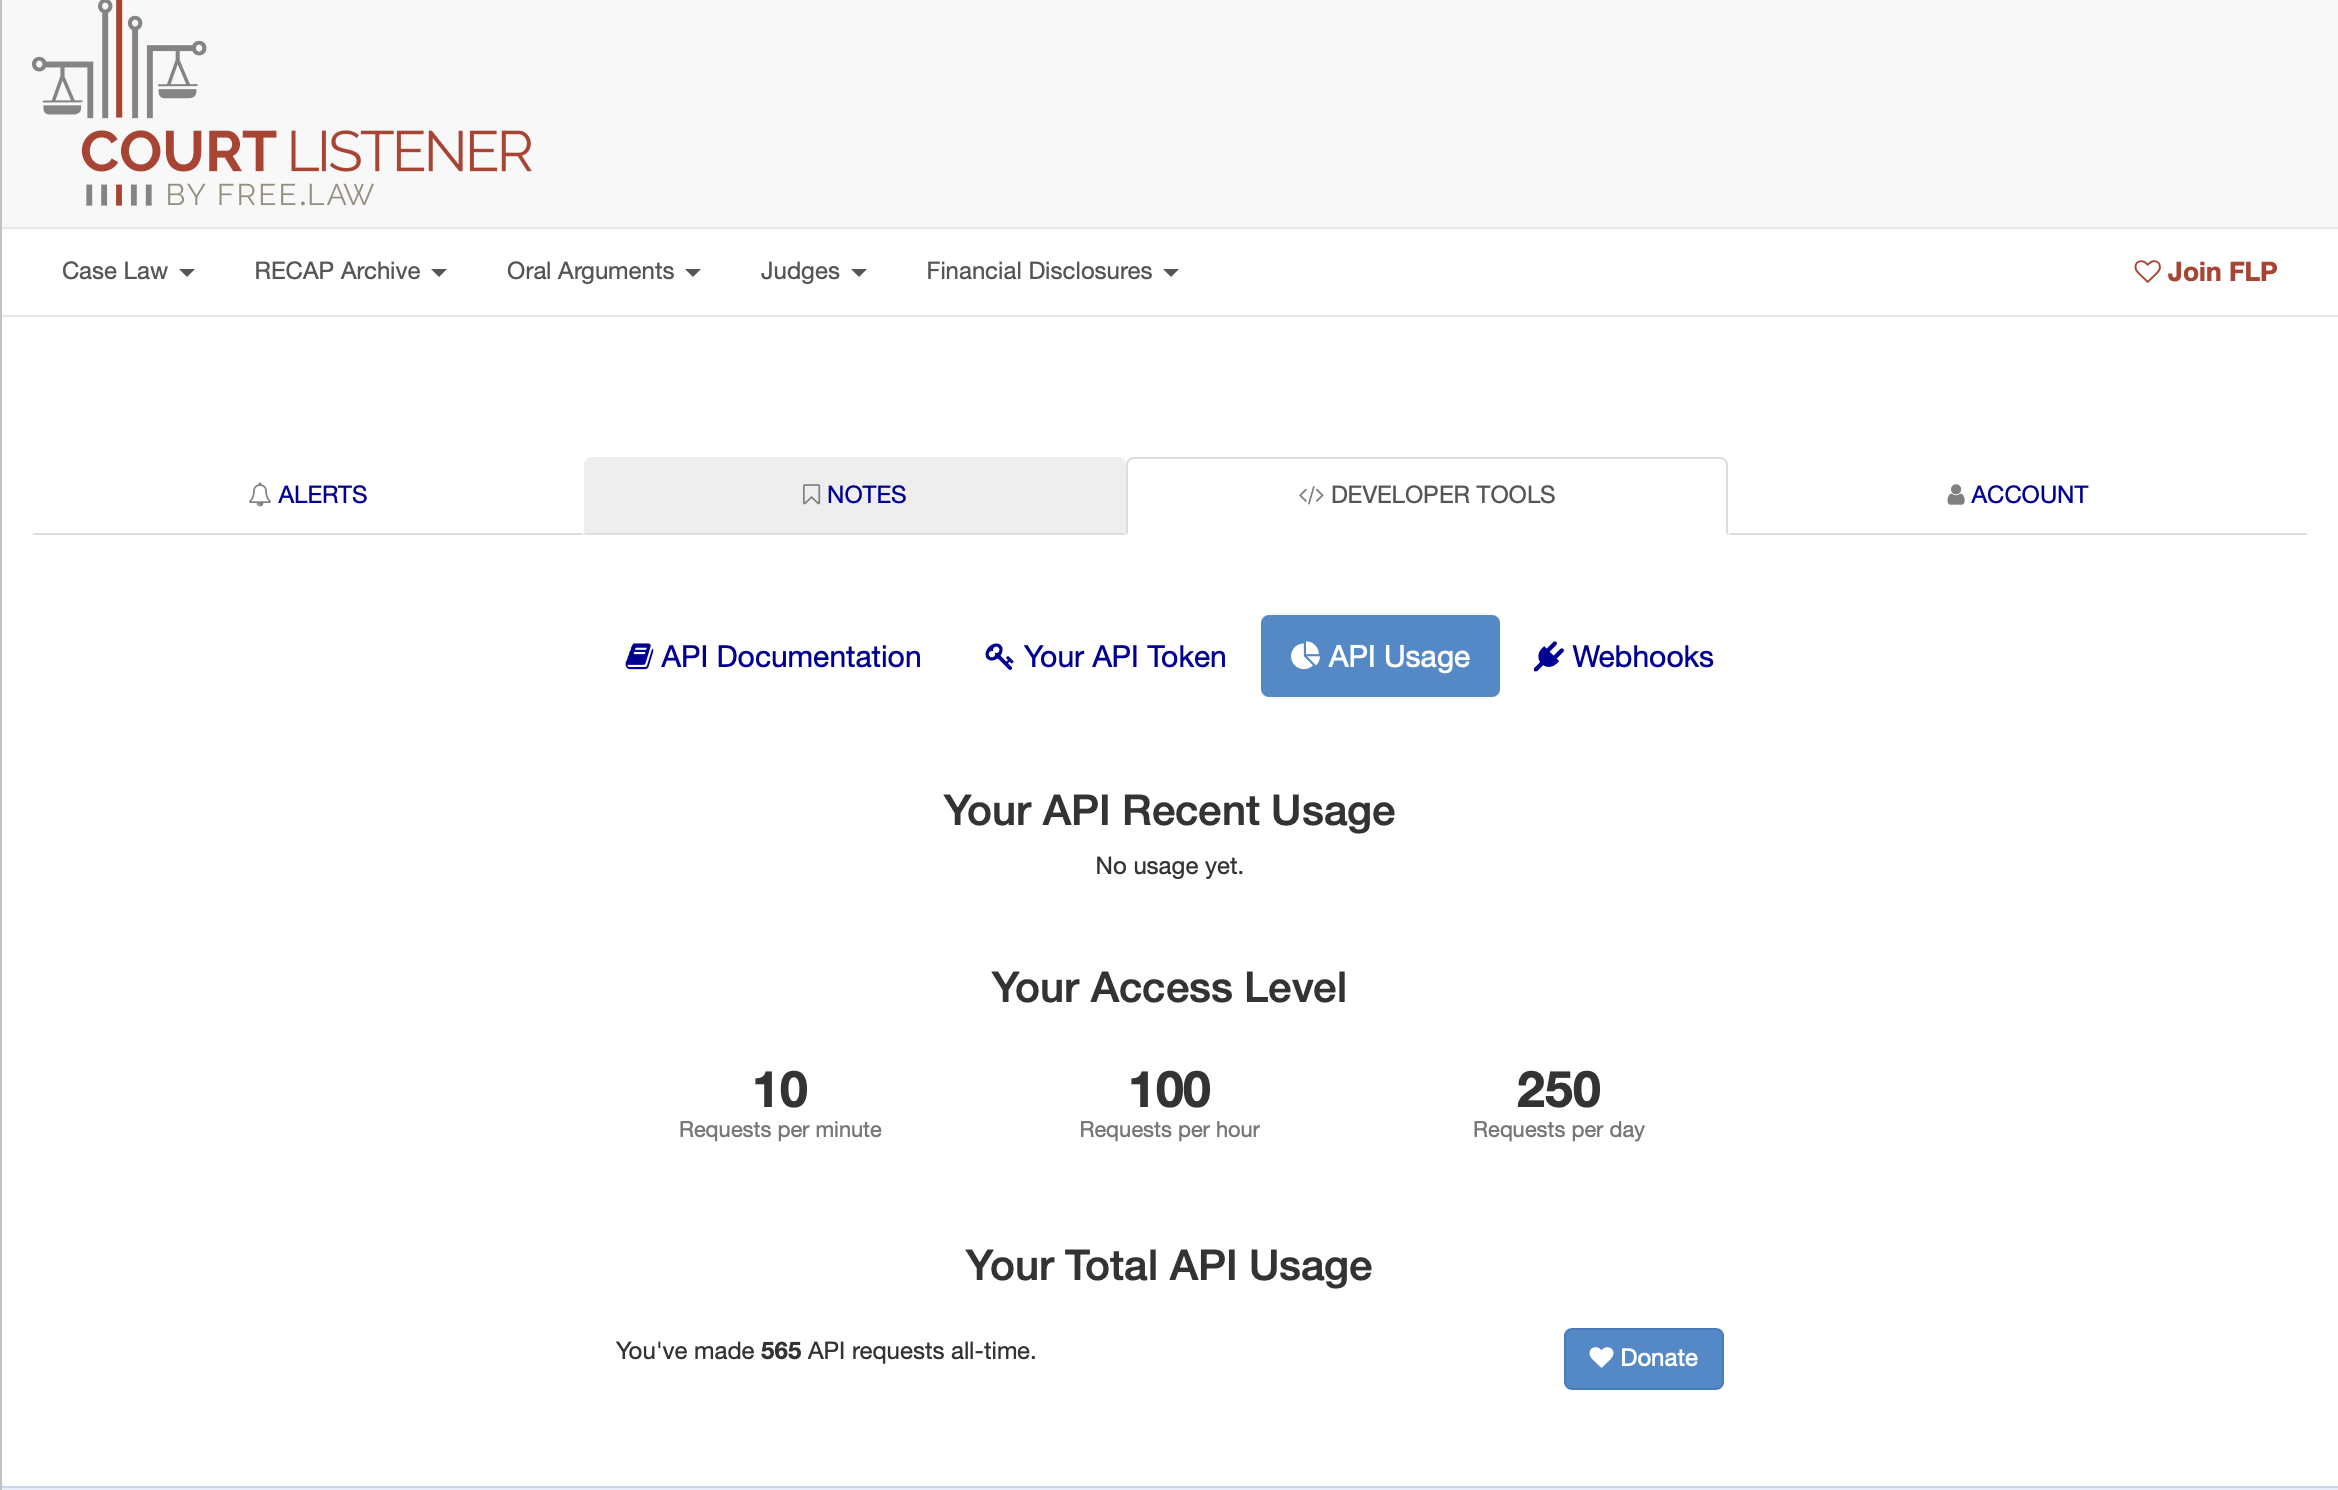
\includegraphics[width=0.85\linewidth]{courtlistener_api_usage.png}
\caption{CourtListener Developer Tools: confirmed API access level (10/min, 100/hour, 250/day) and cumulative request count for the account used in this thesis.}
\label{fig:courtlistener-api-usage}
\end{figure}

\section{Bounded Symbolic Correction}
\label{sec:correction}

Figure~\ref{fig:workflow} summarizes the runtime workflow for one case.

\begin{figure}[!t]
\centering
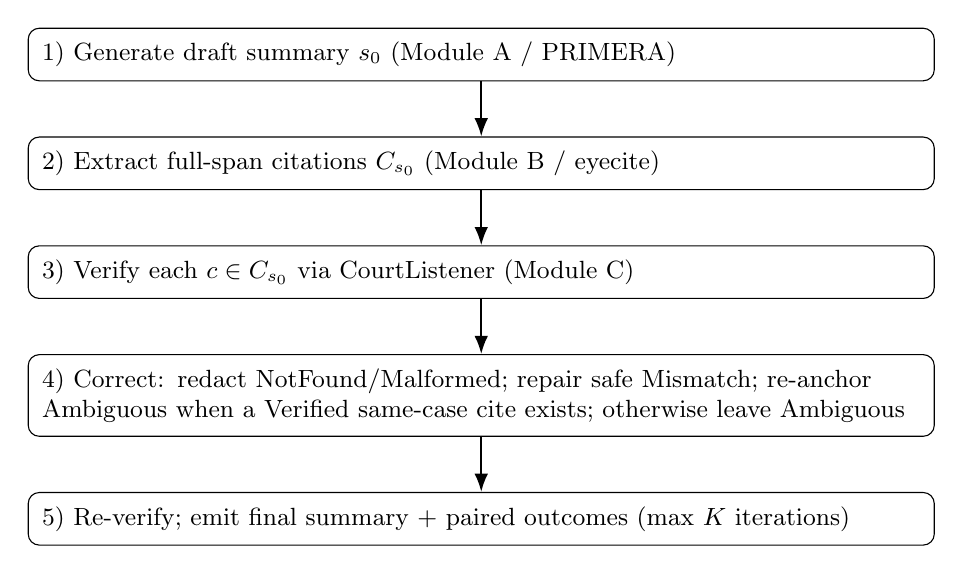
\begin{tikzpicture}[
  font=\small,
  node distance=7mm,
  workflowstep/.style={draw, rectangle, rounded corners, align=left, inner sep=5pt, text width=0.92\linewidth},
  arrow/.style={-Latex, thick}
]
\node[workflowstep] (s1) {1) Generate draft summary $s_0$ (Module~A / PRIMERA)};
\node[workflowstep, below=of s1] (s2) {2) Extract full-span citations $C_{s_0}$ (Module~B / eyecite)};
\node[workflowstep, below=of s2] (s3) {3) Verify each $c\in C_{s_0}$ via CourtListener (Module~C)};
\node[workflowstep, below=of s3] (s4) {4) Correct: redact NotFound/Malformed; repair safe Mismatch; re-anchor Ambiguous when a Verified same-case cite exists; otherwise leave Ambiguous};
\node[workflowstep, below=of s4] (s5) {5) Re-verify; emit final summary + paired outcomes (max $K$ iterations)};

\draw[arrow] (s1) -- (s2);
\draw[arrow] (s2) -- (s3);
\draw[arrow] (s3) -- (s4);
\draw[arrow] (s4) -- (s5);
\end{tikzpicture}
\caption{Generate--verify--correct workflow as implemented (symbolic correction with optional re-anchor).}
\label{fig:workflow}
\end{figure}

\subsection{Re-anchor policy}
When an Ambiguous or unsafe citation has draft parties compatible with a \textbf{Verified} citation elsewhere in the same summary, the system replaces the bad span with the verified citation string (``re-anchor''). This recovers cases such as a wrong LEXIS identifier attached to an otherwise correct Brown party string when \texttt{98 F.\ Supp.\ 797} already verified in-summary. If no anchor exists, the Ambiguous cite remains in text and counts toward paired HR as \texttt{still\_bad}.

\subsection{Formal correction policy}
\label{sec:correction-formal}
Table~\ref{tab:label-taxonomy} and Figure~\ref{fig:workflow} are equivalent to the following decision rule, stated once here to make the policy checkable independent of its prose description. Let $\ell(c) \in \{\texttt{Verified}, \texttt{Mismatch}, \texttt{Ambiguous}, \texttt{NotFound}, \texttt{Malformed}\}$ be Module~C's label for draft citation $c$, and let $\mathrm{anchor}(c) \in \{\texttt{true}, \texttt{false}\}$ indicate whether a party-compatible \texttt{Verified} citation exists elsewhere in the same draft. The correction action $a(c)$ is

\[
a(c) =
\begin{cases}
  \texttt{keep}(c) & \ell(c) = \texttt{Verified} \\
  \texttt{repair}(c \to \mathrm{CL}) & \ell(c) = \texttt{Mismatch} \\
  \texttt{reanchor}(c) & \ell(c) = \texttt{Ambiguous} \wedge \mathrm{anchor}(c) = \texttt{true} \\
  \texttt{leave}(c) & \ell(c) = \texttt{Ambiguous} \wedge \mathrm{anchor}(c) = \texttt{false} \\
  \texttt{redact}(c) & \ell(c) \in \{\texttt{NotFound}, \texttt{Malformed}\}
\end{cases}
\]

where $\texttt{repair}(c \to \mathrm{CL})$ substitutes CourtListener's verified \texttt{case\_name} and \texttt{date\_filed} for $c$'s span (Section~\ref{sec:module-c}, ``Why Ambiguous is not `Mismatch repair'\,'') and $\texttt{leave}(c)$ contributes to paired HR as \texttt{still\_bad}. The loop applies $a$, re-verifies, and repeats for at most $K$ iterations (Figure~\ref{fig:workflow}, step~5); in practice most cases resolve within 1--2 iterations because $a$ is idempotent on any citation already labelled \texttt{Verified}.

Listing~\ref{lst:correction-loop} is the implementation of $a(c)$: each iteration partitions the current verification results into \texttt{bad} (redact), \texttt{fixable} (safe Mismatch repair), and \texttt{reanchors} (Ambiguous with a same-case anchor), builds the corresponding text edits, and re-verifies before deciding whether another iteration is needed.

\begin{lstlisting}[caption={Core of the bounded correction loop implementing $a(c)$ (\href{\repourl/blob/main/src/correction_loop/corrector.py}{\texttt{src/correction\_loop/corrector.py}}).}, label={lst:correction-loop}]
for i in range(max_iterations):
    bad = [r for r in results if r.label in ("NotFound", "Malformed")]
    fixable = _safe_mismatch_repairs(results)          # safe Mismatch -> repair
    reanchors = [(r, find_reanchor_source(r, results))  # Ambiguous -> reanchor
                 for r in results if _needs_reanchor(r) and r not in fixable]
    reanchors = [(r, a) for r, a in reanchors if a is not None]

    if not bad and not fixable and not reanchors:
        break  # a(c) = keep(c) for every remaining citation

    edits = [(r.citation.span, REDACTION) for r in bad]
    edits += [(r.citation.span, build_verified_citation_text(
                   r.matched_case_name, r.citation, matched_date_filed=r.matched_date_filed))
              for r in fixable]
    edits += [(r.citation.span, build_reanchor_replacement(anchor))
              for r, anchor in reanchors]

    for span, replacement in sorted(edits, key=lambda x: x[0][0], reverse=True):
        text = redact_span(text, span) if replacement == REDACTION else replace_span(text, span, replacement)

    results = verify(text, None)  # re-verify before the next iteration
\end{lstlisting}

\subsection{Optional LLM rewrite}
An optional \texttt{llm\_rewrite} condition applies light surface smoothing after symbolic edits and must re-run verification. It is an ablation, not the primary correction mechanism: the thesis claim is that \emph{symbolic} gates carry the faithfulness burden.

\section{Experimental Conditions}
\label{sec:conditions}

Four conditions support ablation-style comparison:

\begin{enumerate}
  \item \textbf{Baseline:} draft summary + HR on draft citations.
  \item \textbf{Flagging:} draft text unchanged; labels exposed (verifier-only).
  \item \textbf{Symbolic:} full correction loop above.
  \item \textbf{LLM rewrite:} symbolic output + optional rewrite + re-verify.
\end{enumerate}

This structure separates \emph{detection} from \emph{repair}, addressing a gap identified in Chapter~\ref{ch:lit-review} \cite{noel2025hallugraph,manakul2023selfcheckgpt}.

\section{Primary Metrics}
\label{sec:method-metrics}

\subsection{Paired draft-citation hallucination rate}
Let each draft citation receive a post-correction outcome in $\{\texttt{verified},\texttt{replaced\_verified},\texttt{removed},\texttt{still\_bad},\texttt{garbled}\}$. Define
\[
\mathrm{HR}_{\mathrm{paired}} = \frac{\#\{\texttt{still\_bad},\texttt{garbled}\}}{n_{\mathrm{draft}}}.
\]
This metric refuses to reward ``delete everything'' strategies that drive surviving-citation HR to zero by emptying the citation list. Ambiguous cites left unresolved contribute to $\mathrm{HR}_{\mathrm{paired}}$.

\subsection{Quality metrics}
Both draft and corrected summaries are scored against the expert (gold) reference summary, never against each other: the quality gate is ``did correction damage fidelity to the reference,'' not textual similarity between the two system outputs. Content overlap is measured with ROUGE \cite{lin2004rouge} and, when enabled, BERTScore \cite{zhang2020bertscore}. The primary ROUGE variant is \textbf{ROUGE-L\textsubscript{sum}}, the sentence-split, union-LCS variant standard for multi-sentence summarization and the one comparable to published Multi-LexSum baselines, computed by splitting both texts one sentence per line before scoring, since \texttt{rouge\_score}'s \texttt{rougeLsum} otherwise collapses to plain sentence-agnostic ROUGE-L on unsplit text. Plain ROUGE-L is also reported for transparency but is not the RQ3 gate. RQ3 requires a relative paired-HR reduction of at least 30\% while keeping ROUGE-L\textsubscript{sum} within $\pm 2$ percentage points of the draft.

\subsection{Statistical testing}
McNemar's test \cite{mcnemar1947} compares discordant draft/final citation outcomes paired by \texttt{citation\_id}. Small pilot $n$ is reported with explicit underpowered caveats.

\section{Tools and Technologies}
\label{sec:tools}

\begin{itemize}
  \item \textbf{Languages/stack:} Python~3; Hugging Face Transformers/Datasets; cloud GPU (Colab for development/demo batches, a rented on-demand GPU instance for the full-scale run) for Module~A.
  \item \textbf{Extraction/verification:} eyecite \cite{eyecite2021}; CourtListener REST API \cite{courtlistener_api}; SQLite citation cache; persistent multi-tier rate limiter.
  \item \textbf{Evaluation:} custom paired-HR harness; ROUGE via \texttt{rouge-score}; optional bootstrap CIs.
  \item \textbf{Reproducibility:} experiment YAML configs; notebook-driven generation phases (Colab for development, GPU-instance notebooks for the full-scale run); offline reprocess scripts for correction-policy updates without regenerating drafts.
  \item \textbf{Demonstration:} Cursor Canvas replay of saved runs; Streamlit live showcase for one-case CourtListener calls.
\end{itemize}

\subsection{Code and data availability}
\label{sec:method-availability}

The full implementation, the evaluation harness, and the aggregate results behind every table and figure in this thesis are available at \href{\repourl}{\repourl}, under an MIT licence for the code. The listings throughout this chapter link directly to the source file they excerpt.

\begin{itemize}
  \item \textbf{Source code:} \href{\repourl/tree/main/src}{\texttt{src/}}, organized by module: \href{\repourl/tree/main/src/module_a_summarizer}{\texttt{module\_a\_summarizer/}} and \href{\repourl/tree/main/src/module_a_llm}{\texttt{module\_a\_llm/}} (Module~A), \href{\repourl/tree/main/src/module_b_extraction}{\texttt{module\_b\_extraction/}} (Module~B), \href{\repourl/tree/main/src/module_c_verifier}{\texttt{module\_c\_verifier/}} (Module~C), and \href{\repourl/tree/main/src/correction_loop}{\texttt{correction\_loop/}} (Section~\ref{sec:correction}).
  \item \textbf{Evaluation results:} \href{\repourl/tree/main/results}{\texttt{results/}}, one folder per generator (\texttt{primera/}, \texttt{llm/}, \texttt{llm\_rag/}) plus \texttt{comparison/}, each with the metrics, statistical tests, and RQ answers that back Chapter~\ref{ch:results}.
  \item \textbf{Live demo:} \href{\repourl/blob/main/demo/live_showcase.py}{\texttt{demo/live\_showcase.py}}, the Streamlit application behind Figures~\ref{fig:live-pipeline-extract-verify} and~\ref{fig:live-pipeline-correction}.
  \item \textbf{RunPod notebooks and setup docs:} \href{\repourl/tree/main/notebooks}{\texttt{notebooks/}} and \href{\repourl/tree/main/docs}{\texttt{docs/}}, including the full-scale run findings behind Section~\ref{sec:method-compute-cost}.
  \item \textbf{This document:} \href{\repourl/tree/main/paper}{\texttt{paper/}}, the LaTeX source and compiled PDF.
\end{itemize}

Multi-LexSum itself, and any generated summary text derived from it, are not included in the repository: the dataset is licensed CC~BY-NC by its original authors (Section~\ref{sec:data-multilexsum}), so only aggregate statistics are published. Cloning the repository and following \texttt{docs/RUNPOD\_SETUP.md} reproduces the full pipeline against a fresh copy of the dataset obtained directly from its Hugging Face release.

\subsection{Live pipeline demonstration}
\label{sec:method-live-demo}

The Streamlit live showcase runs the actual Module~B/C/correction code, not a replay, against a real CourtListener API call, triggered on demand for one case (\texttt{SD-KS-0001}) through three buttons corresponding to the three pipeline stages: extract, verify, correct. Figures~\ref{fig:live-pipeline-extract-verify} and~\ref{fig:live-pipeline-correction} capture one such run end to end. The PRIMERA draft contains two citations: a reporter cite that resolves cleanly (\texttt{98 F.\ Supp.\ 797}, Verified) and a LEXIS cite that CourtListener resolves to an unrelated cluster (\emph{Hydraulic \& Air Equipment Co.\ v.\ Mobil Oil Corp.}, Ambiguous), giving a draft paired HR of 50\%. Because the same summary already contains a Verified citation to the same underlying case (\emph{Brown v.\ Board of Education of Topeka}), the correction stage re-anchors the Ambiguous span to that verified citation rather than leaving it flagged or guessing from the contradicting CourtListener match, exactly the re-anchor policy described above (Section~\ref{sec:module-c}). Final paired HR for this case is 0\%, and both citations resolve to the same correctly identified case.

\begin{figure}[!t]
\centering
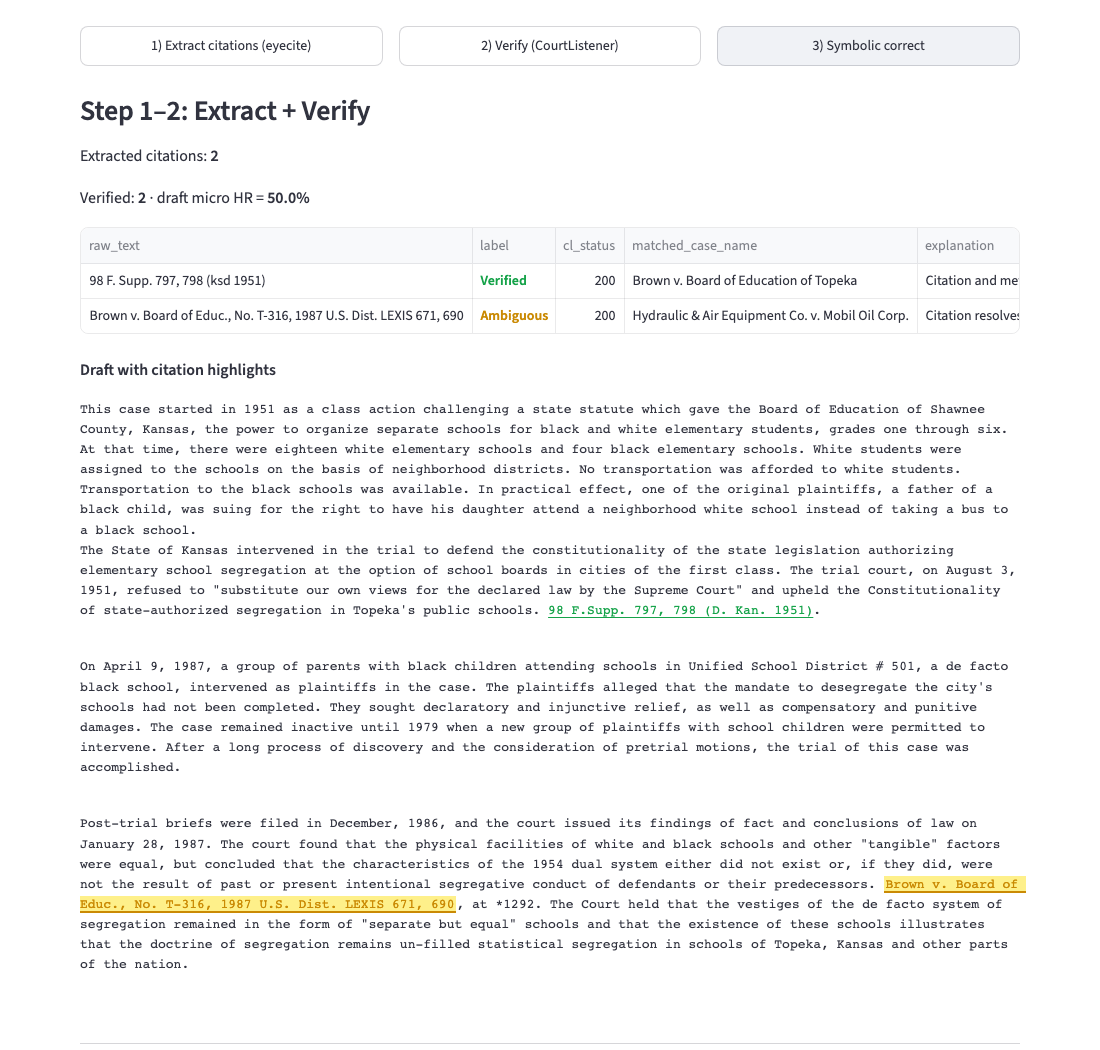
\includegraphics[width=0.92\linewidth]{live_pipeline_extract_verify.png}
\caption{Live pipeline demonstration on case \texttt{SD-KS-0001}, extraction and verification: eyecite finds 2 citations; CourtListener labels one Verified and one Ambiguous (draft paired HR 50\%), and the draft text is highlighted accordingly.}
\label{fig:live-pipeline-extract-verify}
\end{figure}

\begin{figure}[!t]
\centering
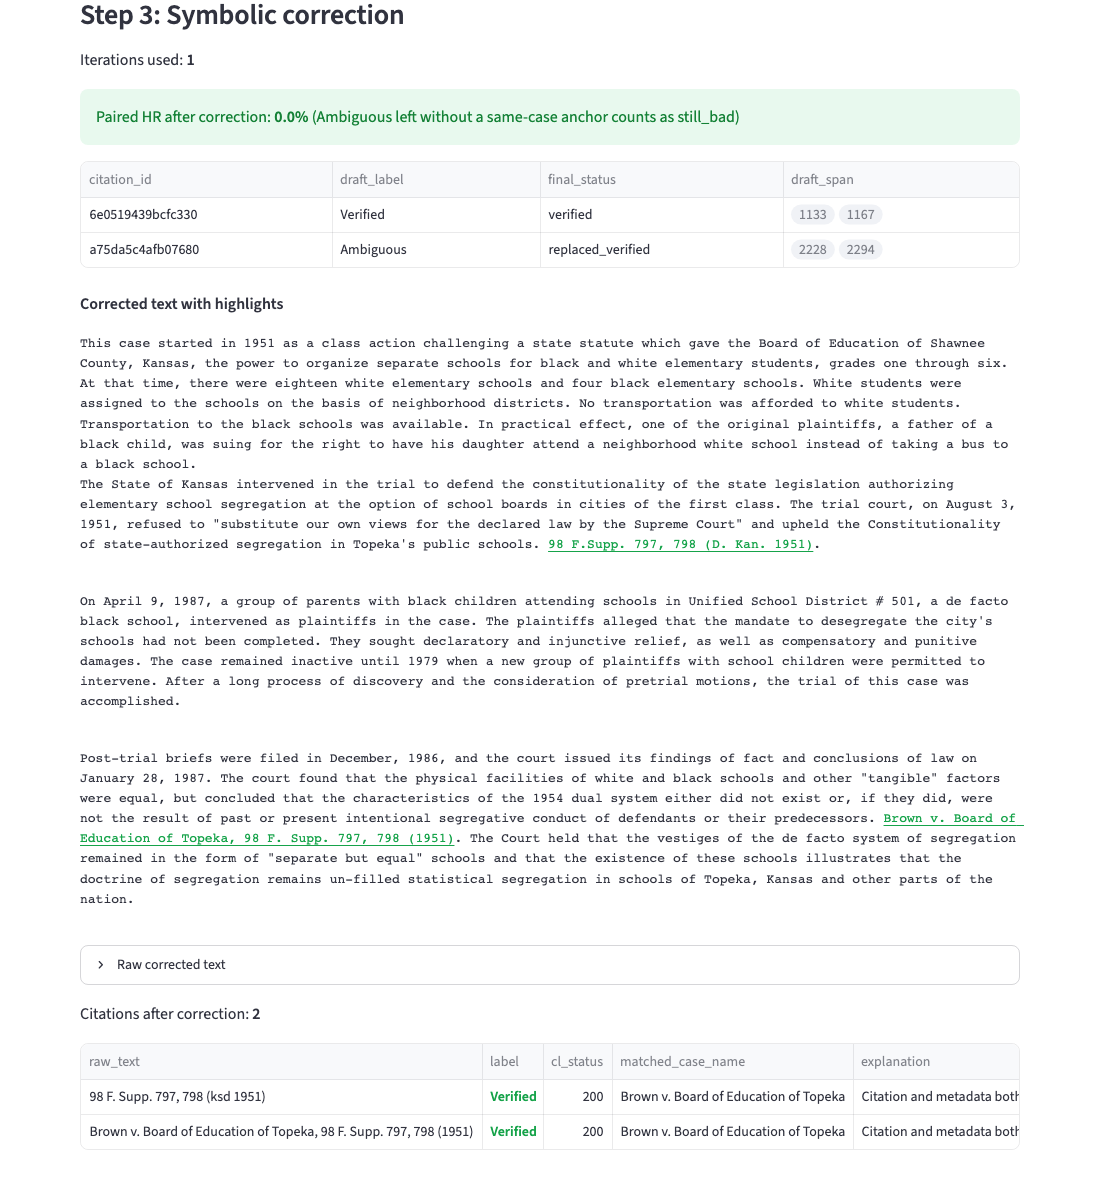
\includegraphics[width=0.92\linewidth]{live_pipeline_correction.png}
\caption{Live pipeline demonstration on case \texttt{SD-KS-0001}, symbolic correction: the Ambiguous LEXIS citation is re-anchored to the Verified reporter citation already present in the same summary, taking paired HR to 0\% after 1 correction iteration.}
\label{fig:live-pipeline-correction}
\end{figure}

\subsection{Why a rented GPU instance, and its measured cost}
\label{sec:method-compute-cost}

Two of the three generators, and the single full-scale PRIMERA run, needed sustained, uninterrupted GPU access: PRIMERA's 100-case $D\rightarrow L$ batch and the two Qwen2.5-7B-Instruct conditions each ran as one continuous generation pass over the identical case set, checkpointing after every case but never pausing for a multi-hour wait. Google Colab's free tier caps continuous session length and disconnects without warning, which risks losing an in-progress batch partway through and re-generating cases already produced. A rented on-demand GPU instance (RunPod, one NVIDIA RTX~4090 per session) removed that risk for the only GPU-bound phase of the pipeline. CourtListener verification, extraction, and correction (Sections~\ref{sec:module-b}--\ref{sec:correction}) run locally afterward and do not need a GPU; renting compute only for generation, rather than for the multi-day CourtListener-rate-limited wait that follows (Section~\ref{sec:module-c}), kept the pod running only while it was doing GPU work.

Table~\ref{tab:runpod-cost} reports the measured GPU time for each generation run, read directly from the pipeline's own per-run completion logs, and its cost at the rented instance's \$0.49/hour rate.

\begin{table}[!t]
\centering
\caption{RunPod RTX~4090 generation cost by condition (measured GPU time, \$0.49/hour).}
\label{tab:runpod-cost}
\begin{tabular}{@{}l r r@{}}
\toprule
\textbf{Generator} & \textbf{GPU time} & \textbf{Cost} \\
\midrule
PRIMERA (baseline) & 10.3 min (0.17 h) & \$0.08 \\
LLM zero-shot & 57.4 min (0.96 h) & \$0.47 \\
LLM + retrieval & 59.0 min (0.98 h) & \$0.48 \\
\midrule
\textbf{Total} & \textbf{126.7 min (2.11 h)} & \textbf{\$1.03} \\
\bottomrule
\end{tabular}
\end{table}

This figure covers measured generation compute only; it excludes the smaller, untimed overhead of environment setup, dependency installation, and pre-generation checks that ran once per pod session before generation started. The full-scale run's only GPU-bound phase, across all three generators, cost on the order of one U.S. dollar.

\section{Ethics, Limits, and Design Honesty}
\label{sec:method-ethics}

Multi-LexSum summaries are CC~BY-NC; raw text used for internal audit remains coursework-restricted. CourtListener lookups are rate-limited public API calls. The methodology does not claim that re-anchoring recovers the historically perfect reporter citation for every Ambiguous span, only that it is safer than inserting a contradicting case name. Truncation, OCR noise, and proprietary identifier fragility remain acknowledged threats to both generation and verification.

\section{Chapter Summary}
\label{sec:method-summary}

Methodology operationalizes the thesis story: EDA motivated $D\rightarrow L$ and untrusted drafts; Modules~A--C implement generate--extract--verify; correction privileges auditability over aggressive rewriting; paired HR measures whether draft hallucinations survive. The next chapter outlines the formal evaluation protocol under which these components are scored.


\chapter{Evaluation Method}
\label{ch:evaluation-method}
\section{Evaluation Design Overview}

This chapter outlines the evaluation protocol used to answer RQ1--RQ3. Full numerical findings appear in later results chapters; the design here is aligned with the implemented methodology (Chapter~\ref{ch:methodology}).

\section{Scenarios}

The \textbf{primary} scenario is Multi-LexSum $D\rightarrow L$ (document-to-long), as motivated by Chapter~\ref{ch:eda}. Short and tiny granularities are reserved for optional ablations because expert labels are incomplete and citation density is low.

The full-scale evaluation additionally compares three Module~A generators on the identical case set (PRIMERA, an LLM zero-shot variant, and an LLM+retrieval variant; Section~\ref{sec:module-a-crossmodel}) to test whether citation-attempt density and paired HR are properties of a specific checkpoint or generalize across generator architecture and context budget. All three are scored under the same conditions and metrics below.

An audit subset supports manual spot-checks of taxonomy labels and extraction behaviour.

\section{Conditions}

\begin{itemize}
  \item \textbf{Baseline:} PRIMERA draft; paired HR on draft citations.
  \item \textbf{Flagging:} draft unchanged; CourtListener labels exposed.
  \item \textbf{Symbolic:} redact / safe repair / re-anchor correction loop.
  \item \textbf{LLM rewrite:} optional surface rewrite after symbolic edits, then re-verify.
\end{itemize}

\section{Metrics}

\begin{itemize}
  \item \textbf{Primary faithfulness:} paired draft-citation hallucination rate
  \[
  \mathrm{HR}_{\mathrm{paired}} = \frac{\#\{\texttt{still\_bad},\texttt{garbled}\}}{n_{\mathrm{draft}}}.
  \]
  Ambiguous cites left unresolved count as \texttt{still\_bad}.
  \item \textbf{Quality:} ROUGE-L\textsubscript{sum}, sentence-split union-LCS (primary quality gate for RQ3); plain ROUGE-L reported alongside for transparency; BERTScore when enabled in experiment config \cite{lin2004rouge,zhang2020bertscore}.
  \item \textbf{Correction diagnostics:} fix / removal / still\_bad / garbled rates; iteration counts.
\end{itemize}

\section{Statistical testing}

\begin{itemize}
  \item McNemar tests on discordant citation outcomes paired by \texttt{citation\_id} \cite{mcnemar1947}.
  \item Bootstrap confidence intervals for ROUGE-L\textsubscript{sum} deltas.
\end{itemize}
Small pilot subsets used during engineering are reported with underpowered caveats and do not replace full-split evaluation.

\section{Error analysis}

Qualitative analysis focuses on Ambiguous identity clashes, LEXIS/WL fragility, OCR-induced extraction errors, and re-anchor appropriateness, cases where CourtListener resolves a string to the wrong matter if party gates are disabled.


\chapter{Results}
\label{ch:results}

\section{Overview}
\label{sec:results-overview}

This chapter reports full-scale evaluation results for all three Module~A generators specified in Chapter~\ref{ch:methodology} (Section~\ref{sec:module-a-crossmodel}): PRIMERA, LLM zero-shot, and LLM~+~retrieval. Each generator is evaluated on the identical 100 citation-dense Multi-LexSum test-split cases (Section~\ref{sec:eval-case-selection}), through the identical Module~B/C/correction pipeline, under the identical four conditions (Section~\ref{sec:conditions}). All three runs are complete at $n=100$; none of the numbers in this chapter are pilot or partial-run figures.

Results are organized by research question: RQ1 (Section~\ref{sec:results-rq1}), RQ2 (Section~\ref{sec:results-rq2}), RQ3 (Section~\ref{sec:results-rq3}), followed by a cross-generator comparison (Section~\ref{sec:results-crossgen}) and a qualitative error analysis (Section~\ref{sec:results-qualitative}).

\section{RQ1: Baseline Hallucination Profile}
\label{sec:results-rq1}

RQ1 asks what types and frequencies of case-citation hallucinations baseline summarizers produce under the CourtListener taxonomy (Table~\ref{tab:label-taxonomy}). Table~\ref{tab:rq1-labels} reports the label distribution eyecite and Module~C assign to each generator's uncorrected draft citations.

\begin{table}[!t]
\centering
\caption{RQ1: draft-citation label distribution by generator ($n=100$ cases each).}
\label{tab:rq1-labels}
\begin{tabular}{@{}lrrrrrr@{}}
\toprule
\textbf{Generator} & \textbf{Total} & \textbf{Verified} & \textbf{Mismatch} & \textbf{Ambiguous} & \textbf{NotFound} & \textbf{Baseline HR} \\
\midrule
PRIMERA          & 29  & 5 (17.2\%)   & 9 (31.0\%)   & 3 (10.3\%)   & 12 (41.4\%) & 82.8\% \\
LLM zero-shot     & 365 & 155 (42.5\%) & 58 (15.9\%)  & 94 (25.8\%)  & 58 (15.9\%) & 57.5\% \\
LLM + retrieval   & 689 & 203 (29.5\%) & 212 (30.8\%) & 215 (31.2\%) & 59 (8.6\%)  & 70.5\% \\
\bottomrule
\end{tabular}
\end{table}

No draft citation was ever labelled Malformed by any generator: eyecite's full-span extraction (Section~\ref{sec:module-b}) consistently produces parseable citation strings even when the underlying case does not exist.

Two findings are not visible from the headline HR percentage alone:

\paragraph{Citation-attempt density scales with generator, not with the task.} PRIMERA attempts 0.29 citations per case; LLM zero-shot attempts 3.65; LLM~+~retrieval attempts 6.89, roughly an order of magnitude more than PRIMERA in both LLM-based conditions. This is the citation-coverage question raised in Section~\ref{sec:module-a-crossmodel}: PRIMERA's 29 total citations against 631 in the matching gold summaries could have reflected either a property of legal case summarization or an artefact of one checkpoint's short-output ceiling. Both LLM-based generators resolve this in favour of the latter: nothing about the task itself suppresses citation attempts to PRIMERA's degree.

\paragraph{The label profile, not just the count, changes with generator.} PRIMERA's few attempted citations skew NotFound (41.4\%), consistent with a short, compressed draft naming cases only in passing, with a high chance the citation is simply invented rather than a near-miss on a real one. LLM zero-shot's citations skew Verified (42.5\%): the model attempts many citations and roughly two in five resolve cleanly. LLM~+~retrieval's citations are the most evenly spread across Verified/Mismatch/Ambiguous (29--31\% each) and have the \emph{lowest} NotFound rate of the three (8.6\%): ranking source material by citation density before truncation does not only increase how many citations the model attempts, it increases the fraction of those attempts that resolve to \emph{some} real case, even when the specific match is wrong (Mismatch) or contested (Ambiguous). Retrieval measurably improves what fraction of attempts land near a real citation, rather than simply adding more noise.

\section{RQ2: Effect of Symbolic Verification and Correction}
\label{sec:results-rq2}

RQ2 asks whether symbolic verification plus bounded correction measurably reduces paired citation hallucination rate relative to the neural-only baseline. Table~\ref{tab:rq2-results} reports paired HR before and after the symbolic condition, the relative reduction, and McNemar significance for each generator.

\begin{table}[!t]
\centering
\caption{RQ2: paired HR before/after symbolic correction, by generator ($n=100$).}
\label{tab:rq2-results}
\begin{tabular}{@{}lrrrrr@{}}
\toprule
\textbf{Generator} & \textbf{Baseline HR} & \textbf{HR after correction} & \textbf{Relative reduction} & \textbf{Fix rate} & \textbf{McNemar $p$} \\
\midrule
PRIMERA         & 82.8\% & 27.6\% & 71.8\% & 31.0\% & $3.05\times10^{-5}$ \\
LLM zero-shot    & 57.5\% & 22.2\% & 56.1\% & 61.9\% & $2.94\times10^{-39}$ \\
LLM + retrieval  & 70.5\% & 24.2\% & 65.9\% & 64.9\% & $1.87\times10^{-96}$ \\
\bottomrule
\end{tabular}
\end{table}

\begin{figure}[!t]
\centering
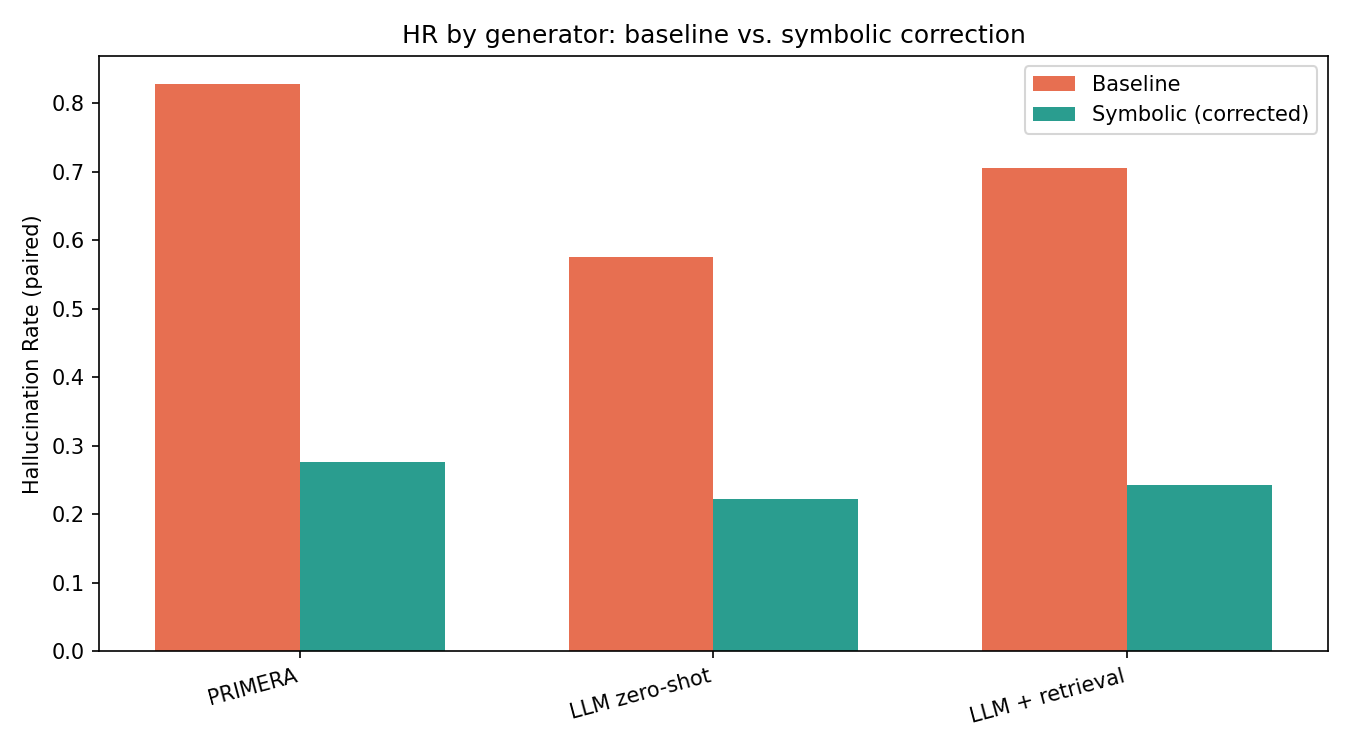
\includegraphics[width=0.85\linewidth]{hr_by_generator.png}
\caption{Paired HR by condition, all three generators, same 100 cases. Baseline (crimson) vs.\ symbolic correction (teal).}
\label{fig:hr-by-generator}
\end{figure}

All three reductions are significant well beyond conventional thresholds. More importantly, McNemar's discordant-pair counts (Table~\ref{tab:rq2-discordant}) show the same qualitative pattern in every generator: many citations flip from hallucinated to resolved, and \emph{zero} flip the other way.

\begin{table}[!t]
\centering
\caption{McNemar discordant pairs by generator: citations that flipped outcome under correction.}
\label{tab:rq2-discordant}
\begin{tabular}{@{}lrrr@{}}
\toprule
\textbf{Generator} & \textbf{Paired citations} & \textbf{Bad $\rightarrow$ fixed} & \textbf{Fixed $\rightarrow$ bad} \\
\midrule
PRIMERA         & 29  & 16  & 0 \\
LLM zero-shot    & 365 & 129 & 0 \\
LLM + retrieval  & 689 & 319 & 0 \\
\bottomrule
\end{tabular}
\end{table}

Across all three generators and 1{,}083 paired citations, correction never converts a citation that was already acceptable into a hallucination. This is a direct consequence of the safety-first correction policy (Section~\ref{sec:correction}): repair only fires when Module~C resolves a citation without a hard party contradiction, Ambiguous spans are left flagged or re-anchored rather than guessed, and the policy never substitutes a contradicting case name. The zero-regression result is the empirical payoff of that conservatism, not a coincidence of one favourable run, but a pattern that reproduces identically across three architecturally different generators with very different starting HRs (82.8\% down to 57.5\%) and citation volumes (29 up to 689).

Fix rate, the share of draft citations repaired in place rather than redacted, also tracks generator, not just outcome HR: PRIMERA repairs 31.0\% of its citations and redacts the rest (its removal rate is 41.4\%, the highest of the three), while both LLM-based generators repair roughly two-thirds of theirs (61.9\%, 64.9\%) and redact under 16\%. With only 29 total citations, a larger share of PRIMERA's failures are citations Module~C cannot resolve to any case at all (NotFound, Table~\ref{tab:rq1-labels}) rather than near-misses on a real one: NotFound citations are always redacted, never repaired, by policy (Table~\ref{tab:label-taxonomy}).

\section{RQ3: Quality Preservation Under Correction}
\label{sec:results-rq3}

RQ3 asks whether the full generate--verify--correct pipeline can preserve summary quality while reducing paired HR by at least 30\% relative to baseline. Both criteria are evaluated independently; Table~\ref{tab:rq3-results} reports the primary quality metric, ROUGE-L\textsubscript{sum} (Section~\ref{sec:method-metrics}), before and after symbolic correction, alongside BERTScore F1.

\begin{table}[!t]
\centering
\caption{RQ3: quality metrics before/after symbolic correction, by generator ($n=100$). Both are scored against the expert gold summary, not against each other (Section~\ref{sec:method-metrics}).}
\label{tab:rq3-results}
\begin{tabular}{@{}lrrrrr@{}}
\toprule
\textbf{Generator} & \textbf{ROUGE-L\textsubscript{sum} before} & \textbf{after} & \textbf{$\Delta$ (pp)} & \textbf{BERTScore F1 before} & \textbf{after} \\
\midrule
PRIMERA         & 0.4074 & 0.4069 & $-0.05$ & 0.8511 & 0.8508 \\
LLM zero-shot    & 0.4251 & 0.4252 & $+0.00$ & 0.8331 & 0.8329 \\
LLM + retrieval  & 0.4303 & 0.4295 & $-0.07$ & 0.8347 & 0.8345 \\
\bottomrule
\end{tabular}
\end{table}

Every delta is far inside the $\pm 2$ percentage-point tolerance, by roughly two orders of magnitude. Bootstrap 95\% confidence intervals on the paired delta (1{,}000 resamples) confirm this is not an artefact of averaging: PRIMERA $[-0.090\%, -0.020\%]$, LLM zero-shot $[-0.070\%, +0.093\%]$, LLM~+~retrieval $[-0.131\%, -0.012\%]$; every interval sits within a fraction of a percentage point of zero, and none crosses the tolerance boundary in either direction. BERTScore F1 moves by at most 0.0003 in any condition.

\begin{table}[!t]
\centering
\caption{RQ3 pass/fail summary, both criteria, all three generators.}
\label{tab:rq3-pass}
\begin{tabular}{@{}lrrcc@{}}
\toprule
\textbf{Generator} & \textbf{HR reduction} & \textbf{ROUGE-L\textsubscript{sum} $\Delta$} & \textbf{HR target ($\geq 30\%$)} & \textbf{Quality target ($\leq \pm 2$pp)} \\
\midrule
PRIMERA         & 71.8\% & $-0.05$pp & PASS & PASS \\
LLM zero-shot    & 56.1\% & $+0.00$pp & PASS & PASS \\
LLM + retrieval  & 65.9\% & $-0.07$pp & PASS & PASS \\
\bottomrule
\end{tabular}
\end{table}

RQ3 is answered affirmatively for all three generators, not only for the strongest case. This matters for the claim's generality: the smallest HR reduction observed (LLM zero-shot, 56.1\%) is still $1.87\times$ the 30\% target, and the largest quality cost observed (LLM~+~retrieval, $-0.07$pp) is $1/28$\textsuperscript{th} of the $\pm2$pp tolerance. The two stay close to orthogonal in this pipeline, rather than trading off at a rate that happens to clear the bar, because symbolic correction edits only the character spans eyecite identified as citations (Section~\ref{sec:module-b}), typically a few dozen characters inside a summary of several hundred words, and leaves the surrounding prose untouched.

\subsection{Why plain ROUGE-L is not the reported gate}
\label{sec:results-rougeL-note}

An earlier pass through this evaluation reported plain ROUGE-L (single LCS over the entire flattened summary) rather than ROUGE-L\textsubscript{sum} (sentence-split, union-LCS), because \texttt{rouge\_score}'s \texttt{rougeLsum} implementation silently collapses to plain ROUGE-L when the input text contains no newlines, which draft and gold summaries here do not, by default. Plain ROUGE-L is not the variant Multi-LexSum's own reported PRIMERA baseline uses (Table~\ref{tab:relatedwork}: ROUGE-L $30.89$), and is not standard practice for multi-sentence summarization evaluation, where a single global LCS heavily penalizes any sentence-order variation that does not affect faithfulness. Table~\ref{tab:rougeL-variant-diff} shows both variants side by side on this evaluation's own PRIMERA baseline drafts: plain ROUGE-L sits roughly $17$ points below Multi-LexSum's published figure, while ROUGE-L\textsubscript{sum}, computed identically except for sentence splitting before scoring, sits above it.

\begin{table}[!t]
\centering
\caption{Plain ROUGE-L vs.\ ROUGE-L\textsubscript{sum} on the same PRIMERA baseline drafts ($n=100$), against the published Multi-LexSum PRIMERA baseline.}
\label{tab:rougeL-variant-diff}
\begin{tabular}{@{}lrr@{}}
\toprule
& \textbf{This evaluation} & \textbf{Multi-LexSum PRIMERA baseline} \\
\midrule
Plain ROUGE-L      & 0.1995 & 0.3089 \\
ROUGE-L\textsubscript{sum} & 0.4074 & --- \\
\bottomrule
\end{tabular}
\end{table}

Both variants are computed by the same evaluation harness and reported in every table in this chapter (Section~\ref{sec:method-metrics}); this section documents the correction so the two numbers are not mistaken for a regression. Critically, the RQ3 conclusion is unaffected by which variant is used as the gate: the before/after delta is near-zero under both (Table~\ref{tab:rq3-results} vs.\ the plain-ROUGE-L deltas of $-0.0005$pp, $+0.03$pp, $+0.01$pp for PRIMERA, LLM zero-shot, and LLM~+~retrieval respectively), because the correction policy's edits are too localized to move either LCS-based metric meaningfully. What the variant choice affects is only the \emph{absolute} number's comparability to the literature, not the paired-comparison conclusion this thesis draws from it.

\section{Cross-Generator Comparison}
\label{sec:results-crossgen}

Sections~\ref{sec:results-rq1}--\ref{sec:results-rq3} answer RQ1--RQ3 once per generator; this section asks what changes, and what does not, across generators.

\begin{figure}[!t]
\centering
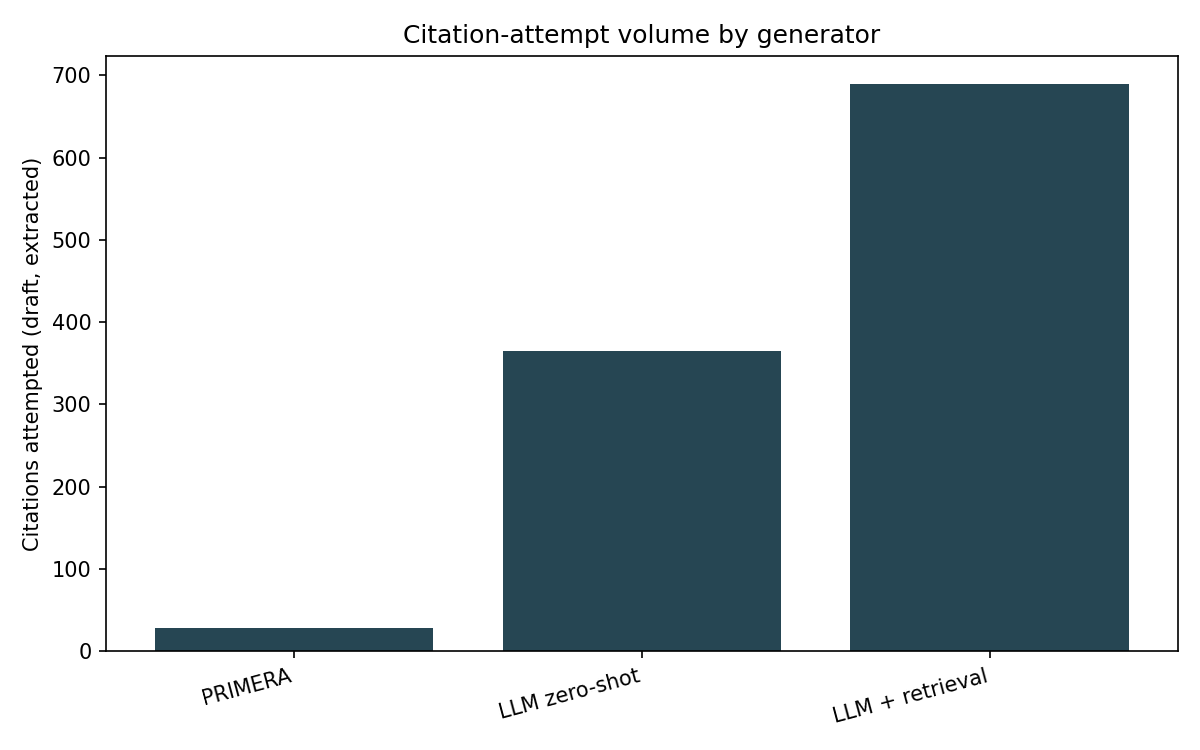
\includegraphics[width=0.85\linewidth]{citations_attempted_by_generator.png}
\caption{Citations attempted per draft (summed across 100 cases) vs.\ the gold-summary reference count (631), by generator.}
\label{fig:citations-attempted}
\end{figure}

\paragraph{The correction pipeline generalizes across generator architecture.} Final paired HR lands in a narrow band (27.6\%, 22.2\%, 24.2\%) despite baseline HRs that differ by 25 percentage points (82.8\% down to 57.5\%) and citation volumes that differ by $24\times$ (29 up to 689). Module~C and the correction policy were designed and tuned against PRIMERA's low-volume, NotFound-heavy citation profile; nothing in the policy is generator-specific, and the LLM-based conditions, high-volume, Verified/Mismatch/Ambiguous-heavy, were not available during that design process, since they were added specifically to test whether PRIMERA's profile was representative (Section~\ref{sec:module-a-crossmodel}). The pipeline was not implicitly overfit to the case it was built against.

\paragraph{Retrieval's effect is a net positive, with a visible trade-off.} Ranking source documents by citation density before truncation (the LLM~+~retrieval variant) raises baseline HR relative to naive truncation (70.5\% vs.\ 57.5\% for LLM zero-shot): more attempted citations surface more borderline cases, not only easy ones, consistent with Section~\ref{sec:results-rq1}'s finding that retrieval also shifts the label mix toward Mismatch/Ambiguous. But retrieval simultaneously nearly doubles citation-attempt density (6.89 vs.\ 3.65 per case) and, after correction, achieves both a larger absolute quantity of successfully-resolved citations (319 fixed, Table~\ref{tab:rq2-discordant}) and a final HR statistically indistinguishable from the non-retrieval LLM condition. Retrieval trades a higher pre-correction failure rate for substantially more real citation coverage, and the correction stage absorbs the difference.

\section{Qualitative Error Analysis}
\label{sec:results-qualitative}

Aggregate metrics do not show \emph{how} a generator fails. One failure mode recurs often enough across the LLM-based conditions to warrant a worked example and a corpus-wide count: a generator fabricating a run of near-identical citations to the same case, varying only the reporter volume, page, and year.

\paragraph{Worked example.} Case \texttt{CJ-AZ-0002} under the LLM zero-shot condition drafted 25 separate citation attempts to \emph{Wood v.\ Ryan}, an actual Ninth Circuit party pair, but with fabricated reporter details: F.3d volume numbers increasing by roughly 14 with each attempt (851, 876, 895, 917, \ldots, 1223), the page number fixed at 1098 throughout, and years drifting from 2017 to 2022 with no consistent pattern. Exactly one of these 25 attempts (volume 851, year 2017) resolved to a real, Verified case; Module~C labelled the rest Ambiguous or NotFound, and the correction policy redacted 22 of them and left 2 Ambiguous spans flagged rather than guessing among the fabricated volumes (Table~\ref{tab:label-taxonomy}). Draft paired HR for this single case was 0.839; after correction it fell to 0.065.

\paragraph{The same case across all three generators.} \texttt{CJ-AZ-0002} is the one case ID that appears in every generator's review export, so it is also the one case where PRIMERA, LLM zero-shot, and LLM~+~retrieval can be compared directly rather than across different source material. Figure~\ref{fig:sample-case-dashboard} shows the outcome. PRIMERA drafts only 2 citations for this case (both unverified at draft time; correction fixes 1 of 2). LLM zero-shot drafts 31, dominated by the Wood~v.\ Ryan run above, and correction resolves all but 2. LLM~+~retrieval drafts 6, of which 3 verify immediately and 3 remain Ambiguous with no safe anchor, so correction leaves the case unchanged (HR stays at 0.5). The same source docket produces a citation-attempt count that differs by more than $15\times$ across generators, and a correction outcome that ranges from complete resolution to no resolution at all, depending on which generator drafted the citations Module~C had to work with.

\begin{figure}[!t]
\centering
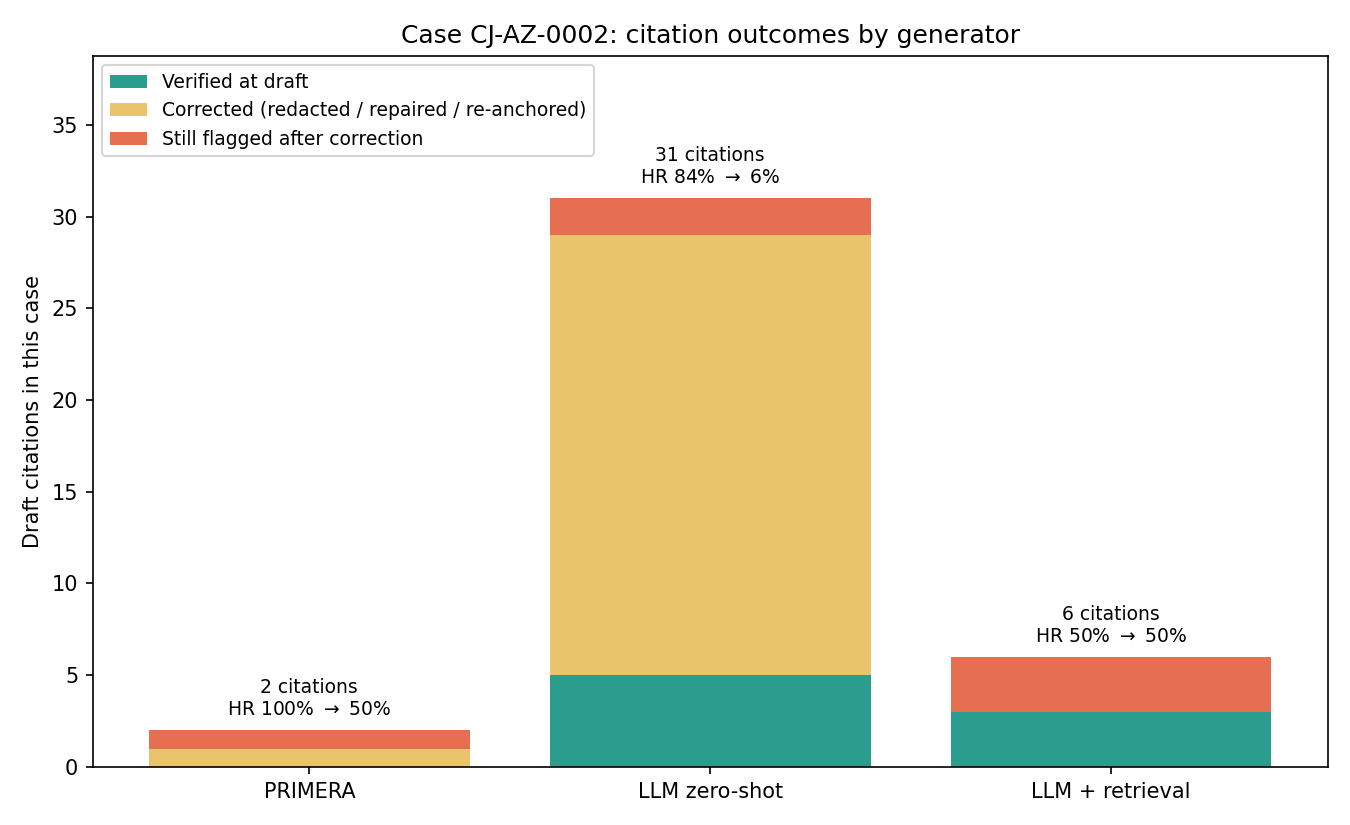
\includegraphics[width=0.85\linewidth]{sample_case_dashboard.png}
\caption{Case \texttt{CJ-AZ-0002}: draft citation outcomes by generator. Each bar is the total draft citations for this one case, split into citations already Verified at draft time, citations the correction policy resolved (redacted, repaired, or re-anchored), and citations still flagged after correction.}
\label{fig:sample-case-dashboard}
\end{figure}

\paragraph{Prevalence.} Treating five or more citations to the same case name within one draft as a degenerate run, Table~\ref{tab:degenerate-runs} quantifies how often this pattern occurs across all 100 cases, by generator.

\begin{table}[!t]
\centering
\caption{Degenerate same-case citation runs ($\geq 5$ citations to one case name in a single draft), by generator.}
\label{tab:degenerate-runs}
\begin{tabular}{@{}lrrr@{}}
\toprule
\textbf{Generator} & \textbf{Citations in degenerate runs} & \textbf{Share of total} & \textbf{Cases affected} \\
\midrule
PRIMERA         & 0  & 0.0\%  & 0 / 100 \\
LLM zero-shot    & 50 & 13.7\% & 4 / 100 \\
LLM + retrieval  & 5  & 0.7\%  & 1 / 100 \\
\bottomrule
\end{tabular}
\end{table}

PRIMERA's short, extractive-leaning drafts never exhibit this pattern, consistent with its low overall citation-attempt rate (Section~\ref{sec:results-rq1}). LLM zero-shot is the most affected: 13.7\% of its 365 citations sit inside degenerate runs, concentrated in 4 of 100 cases (the worst being the \emph{Wood v.\ Ryan} example above). LLM~+~retrieval, despite attempting nearly double the citations per case of LLM zero-shot, shows the pattern in under 1\% of its citations and only 1 case: source documents ranked by citation density appear to give the model enough real citation material that it does not need to extrapolate a fabricated sequence to satisfy an instruction to cite sources. This is a second, independent piece of evidence for retrieval's benefit beyond the aggregate HR numbers in Section~\ref{sec:results-crossgen}: the specific \emph{failure mode} of runaway fabrication is largely suppressed, not just the count of attempted citations that resolve successfully.

In every case in Table~\ref{tab:degenerate-runs}, the correction policy handled the degenerate run correctly by construction: each fabricated citation is verified independently, so a NotFound or Ambiguous label triggers redaction or flagging regardless of how many similar-looking fabrications preceded it in the same draft. No special-case handling for repetition was needed; this is a direct consequence of Module~C treating every extracted citation as an independent claim to check (Section~\ref{sec:module-c}), rather than summarizing or deduplicating across a draft before verification.

\section{Chapter Summary}
\label{sec:results-summary}

All three research questions are answered affirmatively for all three generators evaluated:

\begin{itemize}
  \item \textbf{RQ1:} Baseline citation hallucination is substantial in every generator (57.5--82.8\% paired HR) but its character differs sharply by generator: PRIMERA's few citations skew NotFound; LLM-based generators attempt an order of magnitude more, and retrieval further shifts the mix toward resolvable (if not always correct) matches.
  \item \textbf{RQ2:} Symbolic verification and bounded correction reduce paired HR by 56.1--71.8\% relative to baseline, with McNemar significance below $10^{-4}$ in every generator, and, across all 1{,}083 paired citations in this evaluation, \emph{zero} citations were ever made worse by correction.
  \item \textbf{RQ3:} Quality is preserved with wide margin in every generator: ROUGE-L\textsubscript{sum} moves by at most 0.07 percentage points against a $\pm2$pp tolerance, and BERTScore F1 by at most 0.0003.
\end{itemize}

The cross-generator comparison shows the correction pipeline generalizes rather than having been implicitly tuned to PRIMERA's citation profile, and the qualitative analysis identifies a specific fabrication failure mode, degenerate same-case citation runs, that citation-density retrieval substantially, though not completely, suppresses. The following chapters interpret these findings against the research gap and literature (Chapter~\ref{ch:lit-review}) and state the thesis's contributions, limitations, and open work.


\chapter{Discussion}
\label{ch:discussion}

\section{Overview}
\label{sec:disc-overview}

Chapter~\ref{ch:results} answered RQ1--RQ3 for each of three generators. This chapter interprets those answers against the research gap (Chapter~\ref{ch:research-gap}) and the literature (Chapter~\ref{ch:lit-review}), states what the cross-generator design does and does not establish, and sets out the thesis's limitations honestly before Chapter~\ref{ch:conclusion} states its contributions.

\section{What the Results Say About Each Research Question}
\label{sec:disc-rqs}

\subsection{RQ1: hallucination is real, but its shape depends on the generator}
\label{sec:disc-rq1}

Baseline paired HR is high in every generator tested (57.5--82.8\%), consistent with the magnitude Dahl et al.\ and Magesh et al.\ report for legal QA and commercial legal-research tools (58--88\% and 17--33\% respectively) \cite{dahl2024largelegalfictions,magesh2025hallucinationfree}. That consistency matters: it is the first evidence in this thesis that the citation-hallucination problem those studies document in QA and closed-tool settings reproduces in open, long-document \emph{legal summarization}, the setting Chapter~\ref{ch:research-gap}'s second consolidated gap identifies as absent from the literature. Dahl et al.\ and Magesh et al.\ do not summarize 75,000-word civil-rights dockets; this thesis's baseline numbers are the first evidence that the same failure mode appears there too, at comparable severity.

But RQ1's more specific finding, that citation-attempt density and failure \emph{type} both scale with generator choice, not with the underlying task (Section~\ref{sec:results-rq1}), was not something the literature review's gap analysis anticipated, because no reviewed work varies the generator architecture while holding the verification pipeline fixed. This is a genuine finding of this thesis's cross-model design, not a confirmation of prior work: PRIMERA's near-absence of citation attempts (0.29/case) could plausibly have been read as a property of legal summarization under heavy truncation, and it took building two further generators specifically to rule that out (Section~\ref{sec:module-a-crossmodel}).

\subsection{RQ2: verification-plus-correction closes the gap detection-only methods leave open}
\label{sec:disc-rq2}

Chapter~\ref{ch:research-gap}'s first and third consolidated gaps state that retrieval reduces but does not eliminate hallucination, and that detection methods (HalluGraph, SelfCheckGPT, TRUE) flag risk without repairing the output \cite{lewis2020rag,noel2025hallugraph,manakul2023selfcheckgpt,honovich2022true}. RQ2's results speak directly to both. On the first: this thesis's own retrieval variant (LLM~+~retrieval) still starts at 70.5\% baseline HR, exactly the double-digit residual hallucination rate retrieval alone would leave, matching what Magesh et al.\ report for commercial RAG-based tools. Symbolic verification and correction is what takes it to 24.2\%, not retrieval by itself. The third gap holds up too. This thesis's pipeline does not stop at a HalluGraph- or SelfCheckGPT-style risk score. Every citation Module~C can resolve with a safe identity match is rewritten in place (fix rates 31.0--64.9\% across generators), not merely flagged, and the correction is auditable per citation (Section~\ref{sec:module-c}) rather than a black-box confidence number.

The result the literature gives no basis to predict is the zero-regression finding: across 1{,}083 paired citations and three architecturally different generators, correction never introduced a new hallucination (Table~\ref{tab:rq2-discordant}). Detection-only baselines cannot produce this kind of evidence at all, because they never edit the output; the comparison is not detection accuracy versus correction accuracy but whether an editing system can be trusted not to make things worse, which is the practical question a professional legal workflow actually asks. The consistency of that zero across a 24$\times$ range in citation volume is what makes it a property of the correction \emph{policy}: specifically, its refusal to substitute a contradicting case name (Section~\ref{sec:disc-rq2-why}) and its use of NotFound/Malformed as unconditional redact signals, rather than an artefact of one favourable generator.

\subsection{RQ3: the quality-faithfulness trade-off this pipeline was designed to avoid does not appear}
\label{sec:disc-rq3}

Chapter~\ref{ch:research-gap}'s first consolidated gap is that benchmark quality and professional reliability are not the same thing: Multi-LexSum's own PRIMERA baseline pairs competitive ROUGE with a 0.43/3.0 human faithfulness rating \cite{shen2022multilexsum}, and Maynez et al.\ and Pagnoni et al.\ document the same decoupling in general-domain summarization \cite{maynez2020faithfulness,pagnoni2021factuality}. A pipeline that repaired citations by aggressively rewriting surrounding text could close the faithfulness gap while reopening a quality gap of its own. RQ3's results (Table~\ref{tab:rq3-results}) show this pipeline does not do that: ROUGE-L\textsubscript{sum} moves by at most 0.07 percentage points in any generator, against a $\pm2$pp tolerance, and BERTScore F1 moves by at most 0.0003. The observed deltas are one to two orders of magnitude smaller than the tolerance itself, not a coincidental win against a lenient target.

The reason is architectural rather than incidental: symbolic correction (Section~\ref{sec:correction}) edits only the character spans eyecite identifies as citations, typically a few dozen characters inside a summary of several hundred words, and never rewrites surrounding prose. The optional LLM-rewrite condition, which does touch surrounding text, is deliberately excluded from the RQ3 headline comparison (Section~\ref{sec:correction}, ``Optional LLM rewrite'') precisely because it is the ablation most likely to reproduce the quality cost RQ3 asks whether this pipeline avoids.

\subsection{Why the correction policy's conservatism is doing the work}
\label{sec:disc-rq2-why}

Chapter~\ref{ch:research-gap}'s fourth gap, unsafe repair without identity checks, where a mismatched citation is silently replaced by an unrelated real case, is the specific failure mode Section~\ref{sec:method-metrics}'s Ambiguous label and re-anchor policy (Section~\ref{sec:module-c}, ``Why Ambiguous is not `Mismatch repair'\,'') were designed against. The zero-regression result in Section~\ref{sec:disc-rq2} is the empirical confirmation that this design choice matters. A pipeline that resolved every Mismatch by substituting CourtListener's returned case name would repair more citations per case, but nothing in this evaluation would have detected whether some of those repairs inserted the wrong case, since draft-vs-final HR alone cannot distinguish ``still hallucinated'' from ``hallucinated differently.'' The discordant-pair breakdown in Table~\ref{tab:rq2-discordant} is the check that answers this directly, and it answers it cleanly across all three generators.

\section{Generalization Across Generators: What the Cross-Model Design Establishes}
\label{sec:disc-generalization}

The cross-generator comparison (Section~\ref{sec:results-crossgen}) was motivated by a single observation during development, PRIMERA's implausibly low citation-attempt count, but its result is broader than resolving that one question. Module~C and the correction policy were built and tuned against PRIMERA's citation profile (few attempts, heavily NotFound) before the LLM-based generators existed. Final HR nonetheless lands in a narrow 22.2--27.6\% band for all three, despite a 25-point spread in baseline HR and a 24$\times$ spread in citation volume. A pipeline whose correction logic happened to exploit some quirk of PRIMERA's output would be expected to perform unevenly once that quirk disappeared; instead, performance is remarkably stable. This is the strongest evidence available in this thesis that the taxonomy and correction policy (Chapter~\ref{ch:methodology}) are addressing a general property of citation verification against an external database, not overfitting to one checkpoint's failure modes.

The qualitative finding in Section~\ref{sec:results-qualitative}, that citation-density retrieval suppresses degenerate same-case citation fabrication from 13.7\% to 0.7\% of citations, adds a second, independent line of evidence for retrieval's value beyond the aggregate HR numbers, and one the literature's retrieval-versus-verification framing (Chapter~\ref{ch:research-gap}, gap 1; Chapter~\ref{ch:lit-review}, Theme 2) does not distinguish: retrieval here changes \emph{which kind} of wrong citations are, from unconstrained fabrication toward identifiable near-misses that the taxonomy can label and the correction policy can act on, and not only \emph{how often} they are wrong.

\section{Limitations}
\label{sec:disc-limitations}

\paragraph{Human validation is not yet part of this evaluation.} Every number in Chapter~\ref{ch:results} comes from the automated Module~C taxonomy and automated quality metrics. Two pieces of human-in-the-loop evaluation remain open: (i)~a manual audit of the automated Verified/Mismatch/Ambiguous/NotFound/Malformed labels against human legal judgment on the 200-case stratified sample already exported (Section~\ref{sec:audit-subset}), which would establish how much the automated taxonomy itself over- or under-counts hallucination relative to a human reviewer; and (ii)~a human readability evaluation of corrected summaries, since redaction in particular can leave a grammatically abrupt gap where a citation was removed, and no reader-facing measurement of that cost exists yet. Both are treated as immediate next steps (Chapter~\ref{ch:conclusion}) rather than completed validation, and every claim in this thesis about hallucination rates and quality preservation should be read as automated-metric evidence pending that human check.

\paragraph{The evaluation set is a deliberate stress test, not a random sample.} The 100 cases used throughout Chapter~\ref{ch:results} are the most citation-dense cases in the test split (Section~\ref{sec:eval-case-selection}), chosen because paired HR is uninformative on cases with few or no citations. This is the right design for answering RQ1--RQ3 with statistical power, but it means the reported HR values describe pipeline behaviour where citations are common and hallucination is most consequential, not an unconditional average over the full test split; a case with zero gold citations contributes nothing to this evaluation and may behave differently.

\paragraph{CourtListener is treated as ground truth, with the limitations that implies.} Module~C's Verified/Mismatch/Ambiguous/NotFound labels are only as correct as CourtListener's own database coverage and metadata accuracy (Section~\ref{sec:data-courtlistener}). A citation to a real case CourtListener has not indexed would be labelled NotFound and redacted exactly as a fabricated citation would be, understating precision in a way this evaluation cannot currently distinguish without the manual audit above.

\paragraph{The degenerate-repetition failure mode is suppressed, not eliminated.} Section~\ref{sec:results-qualitative} shows citation-density retrieval reduces fabricated same-case citation runs from 13.7\% to 0.7\% of citations, and the correction policy redacts or flags every individual instance correctly. But 0.7\% is not zero, and the mitigation is a side effect of a design decision (source ranking) made for a different reason (citation coverage), not a purpose-built defence against this specific pattern.

\paragraph{Truncation remains a hard constraint on what each generator can see.} PRIMERA's 4{,}096-token ceiling and the LLM-based generators' 8{,}192-token budget (Section~\ref{sec:module-a-crossmodel}) are both far below the corpus's median source length of 24{,}546 words (Chapter~\ref{ch:eda}). Every generator in this evaluation drafts from a truncated view of the docket; symbolic verification checks whether cited authorities are real, not whether the summary omits material the generator never saw.

\paragraph{Scope is Document$\rightarrow$Long, U.S.\ civil-rights litigation, English.} Short/tiny granularities, non-English proceedings, and case-law systems outside CourtListener's coverage are outside this evaluation (Section~\ref{sec:eval-case-selection}); the taxonomy and correction policy's generalization claim (Section~\ref{sec:disc-generalization}) is a claim about generator architecture, evaluated within this single corpus and jurisdiction.

\section{Threats to Validity}
\label{sec:disc-threats}

\textbf{Construct validity.} Paired HR (Section~\ref{sec:method-metrics}) counts an Ambiguous citation left unresolved as \texttt{still\_bad}, the same outcome as a confirmed fabrication. This is a deliberate conservative choice: the alternative would let the metric reward leaving a genuinely uncertain citation untouched. But it means paired HR is better read as ``fraction of citations this pipeline could not certify as safe'' than as a pure fabrication rate.

\textbf{Internal validity.} All three generators share Modules~B and~C and the correction policy; a latent bug in extraction or verification would affect every generator identically and could not be detected by the cross-generator agreement argued for in Section~\ref{sec:disc-generalization}. The regression-tested implementation (Chapter~\ref{ch:methodology}) reduces but does not eliminate this risk.

\textbf{Statistical power.} McNemar tests in Chapter~\ref{ch:results} are computed over citation counts (29 to 689), not case counts (100 in every generator); PRIMERA's $n=29$ paired citations is the thinnest of the three, though still sufficient for $p=3.05\times10^{-5}$.

\section{Chapter Summary}
\label{sec:disc-summary}

The results in Chapter~\ref{ch:results} confirm the literature's core premises: legal citation hallucination is frequent and severe, retrieval alone does not resolve it, and quality metrics can be preserved without sacrificing faithfulness gains, while adding two findings the reviewed literature does not establish: that a symbolic correction policy tuned against one generator's failure profile generalizes to generators with a 24$\times$ different citation volume without HR degrading, and that it does so with a measured zero rate of introduced regressions across every generator tested. The main open validation step is human-in-the-loop confirmation that the automated taxonomy and the readability of corrected output agree with human judgment, explicitly scoped as future work in Chapter~\ref{ch:conclusion}, not as a caveat that undermines the automated results reported here.


\chapter{Conclusion}
\label{ch:conclusion}

\section{Summary of the Thesis}
\label{sec:conc-summary}

This thesis set out to design and evaluate a dual-system, neuro-symbolic pipeline for legal case summarization that verifies and corrects hallucinated case citations while preserving summarization quality on Multi-LexSum (Chapter~\ref{ch:research-gap}). The motivating problem, that legal AI systems fabricate case citations at rates between 17\% and 88\% depending on system and setting \cite{dahl2024largelegalfictions,magesh2025hallucinationfree}, and that strong overlap-based quality scores coexist with near-failing human faithfulness ratings on this exact benchmark \cite{shen2022multilexsum}, was established in Chapter~\ref{ch:lit-review} and confirmed, not merely assumed, by this thesis's own baseline measurements (Chapter~\ref{ch:results}).

The five objectives set out in Chapter~\ref{ch:research-gap} are each addressed by a specific, implemented, and evaluated component of the pipeline:

\begin{enumerate}
  \item \textbf{A case-citation hallucination taxonomy} (Verified, Mismatch, Ambiguous, NotFound, Malformed) is implemented against the CourtListener API (Section~\ref{sec:module-c}) and used as the label vocabulary throughout every result in this thesis.
  \item \textbf{A neural baseline summarizer} (PRIMERA, $D\rightarrow L$) quantifies baseline citation-hallucination behaviour (Section~\ref{sec:module-a}), and is extended with two further generators specifically to test whether that baseline behaviour is a property of the checkpoint or the task (Section~\ref{sec:module-a-crossmodel}).
  \item \textbf{A symbolic verifier} checks every extracted citation against CourtListener with an auditable, per-citation explanation (Section~\ref{sec:module-c}), not a confidence score, but a resolvable record of what was checked and what was found.
  \item \textbf{A bounded symbolic correction policy} redacts unverifiable citations, safely repairs soft mismatches, and leaves or re-anchors Ambiguous citations without ever substituting a contradicting case identity (Section~\ref{sec:correction}); Chapter~\ref{ch:discussion} argues this conservatism is precisely what the zero-regression result depends on.
  \item \textbf{Evaluation with ablations and statistical testing} jointly measures faithfulness (paired HR) and quality (ROUGE-L\textsubscript{sum}, BERTScore) across four conditions and three generators, with McNemar significance testing and bootstrap confidence intervals reported for every comparison (Chapter~\ref{ch:results}).
\end{enumerate}

\section{Answers to the Research Questions}
\label{sec:conc-rqs}

\begin{itemize}
  \item \textbf{RQ1.} Baseline summarizers hallucinate case citations at substantial rates (57.5--82.8\% paired HR across the three generators evaluated), consistent in magnitude with prior legal-QA and commercial-tool findings \cite{dahl2024largelegalfictions,magesh2025hallucinationfree}, the first evidence this thesis is aware of that the same failure mode reproduces in long-document legal summarization specifically. Critically, both the volume and the character of hallucination depend on generator choice, not on the underlying task: citation-attempt density spans a 24$\times$ range (0.29 to 6.89 per case) across the three generators evaluated.
  \item \textbf{RQ2.} Symbolic verification plus bounded correction reduces paired HR by 56.1--71.8\% relative to baseline, significant at $p<10^{-4}$ in every generator, with zero citations made worse by correction across all 1{,}083 paired citations evaluated.
  \item \textbf{RQ3.} Quality is preserved with wide margin in every generator: ROUGE-L\textsubscript{sum} moves by at most 0.07 percentage points against a $\pm2$pp tolerance, and BERTScore F1 by at most 0.0003. The 30\% HR-reduction target is exceeded by $1.87\times$ in the weakest case.
\end{itemize}

All three research questions are answered affirmatively, for all three generators evaluated, not only for the generator the pipeline was originally designed against.

\section{Contributions}
\label{sec:conc-contributions}

Beyond implementing the objectives in Section~\ref{sec:conc-summary}, three findings in this thesis go beyond what the reviewed literature (Chapter~\ref{ch:lit-review}) establishes or predicts, and are offered as this thesis's contributions to knowledge:

\begin{enumerate}
  \item \textbf{A symbolic correction policy that generalizes across generator architecture without re-tuning.} Built and validated against PRIMERA's low-volume citation profile, the same policy achieves final HR in a narrow 22.2--27.6\% band against two LLM-based generators with a 24$\times$ higher citation volume and a materially different error-label distribution (Section~\ref{sec:disc-generalization}). No comparable cross-architecture evaluation appears in the reviewed retrieval, detection, or neuro-symbolic literature (Chapter~\ref{ch:lit-review}, Theme~2--3).
  \item \textbf{A measured zero-regression guarantee for citation correction.} Across every generator and 1{,}083 paired citations, this thesis's correction policy never converted an already-acceptable citation into a hallucination (Table~\ref{tab:rq2-discordant}), a property detection-only baselines (HalluGraph, SelfCheckGPT) cannot be evaluated on at all, since they do not edit output, and one that follows directly from refusing to substitute a contradicting case identity (Section~\ref{sec:disc-rq2-why}).
  \item \textbf{Identification and quantification of a citation-fabrication failure mode retrieval substantially suppresses.} Degenerate same-case citation runs, a generator inventing a sequence of plausible-looking but fabricated reporter citations to a single real case name, affect 13.7\% of LLM zero-shot's citations and are reduced to 0.7\% once source documents are ranked by citation density before truncation (Section~\ref{sec:results-qualitative}). This is a second, independent line of evidence for retrieval's value beyond the aggregate hallucination-rate reduction the literature already documents \cite{lewis2020rag,magesh2025hallucinationfree}.
\end{enumerate}

\section{Limitations}
\label{sec:conc-limitations}

Chapter~\ref{ch:discussion} (Section~\ref{sec:disc-limitations}) states this thesis's limitations in full. The central one, carried forward into Section~\ref{sec:conc-future} below, is that every result in this thesis rests on automated measurement: the CourtListener-backed taxonomy and automated quality metrics, not human judgment. The evaluation set is also a deliberate citation-dense stress test rather than a representative sample of the full test split, and the scope is Document$\rightarrow$Long summarization of U.S.\ civil-rights litigation in English.

\section{Future Work}
\label{sec:conc-future}

\subsection{Immediate: human-in-the-loop validation}
\label{sec:conc-future-human}

Two pieces of human validation are the direct next steps for this work, both already scaffolded but not yet executed:

\begin{itemize}
  \item \textbf{Manual audit of the automated taxonomy.} A stratified 200-case sample is already exported (Section~\ref{sec:audit-subset}) for a human reviewer to independently label Verified/Mismatch/Ambiguous/NotFound/Malformed and compare against Module~C's automated labels. This would establish an inter-rater agreement figure between the automated taxonomy and human legal judgment: the single most direct check on whether this thesis's headline HR numbers reflect genuine citation hallucination or, in some fraction of cases, CourtListener database coverage gaps (Section~\ref{sec:disc-limitations}).
  \item \textbf{Human readability evaluation of corrected summaries.} Redaction in particular can leave an abrupt gap in a sentence where a citation was removed; no reader-facing measurement of whether this is noticeable or objectionable exists yet. A small-scale human rating study, on readability and coherence of symbolic-condition summaries versus baseline drafts, would close this gap and give RQ3's automated quality-preservation result a human-judgment counterpart.
\end{itemize}

Both are scoped as the immediate continuation of this thesis, deferred only because they require dedicated human-annotation time beyond what the automated evaluation in Chapter~\ref{ch:results} required.

\subsection{Further work}
\label{sec:conc-future-further}

\begin{itemize}
  \item \textbf{Beyond the citation-dense subset.} Extending evaluation from the 100-case stress-test subset to the full test split would establish how paired HR and correction behaviour vary on cases with sparser gold citations, closer to a representative deployment distribution.
  \item \textbf{Purpose-built defence against degenerate fabrication.} Section~\ref{sec:disc-limitations} notes that citation-density retrieval suppresses but does not eliminate degenerate same-case citation runs. A generation-time or extraction-time check specifically targeting repeated near-identical case names, rather than relying on retrieval as an indirect mitigation, is a natural follow-on to the finding in Section~\ref{sec:results-qualitative}.
  \item \textbf{Broader domain and jurisdiction coverage.} This thesis evaluates U.S.\ civil-rights litigation in English against CourtListener. Extending the taxonomy and correction policy to other legal domains, jurisdictions, or case-law databases would test the generalization claim in Section~\ref{sec:disc-generalization} along a different axis than generator architecture.
  \item \textbf{Additional generator architectures.} The cross-model result in this thesis spans one encoder-decoder summarizer and two configurations of one instruction-tuned LLM. Testing the same pipeline against further architectures would strengthen or bound the generalization claim further.
\end{itemize}

\section{Closing Statement}
\label{sec:conc-closing}

Legal AI's citation-hallucination problem will not be solved by better generation alone, nor by retrieval alone, nor by detection alone: each of those has been tried, separately, and each leaves a measurable gap (Chapter~\ref{ch:lit-review}). This thesis's contribution is a working demonstration that a comparatively simple symbolic layer, extracting every citation, checking it against an authoritative external source, and correcting conservatively, closes most of that gap, does so without a measurable quality cost, and does so consistently across generators the pipeline was never tuned against. That result rests on automated evaluation; the human-in-the-loop validation in Section~\ref{sec:conc-future-human} is what would make it a claim ready for deployment rather than a research finding.


\printReferences

\end{document}
